\subsection{Results on Efficiency}
\label{efficiency}

\begin{figure*}[htp]
\hspace*{-.4cm}
\centering
\begin{tabular}{c c c c}
  \begin{minipage}{3.76cm}
	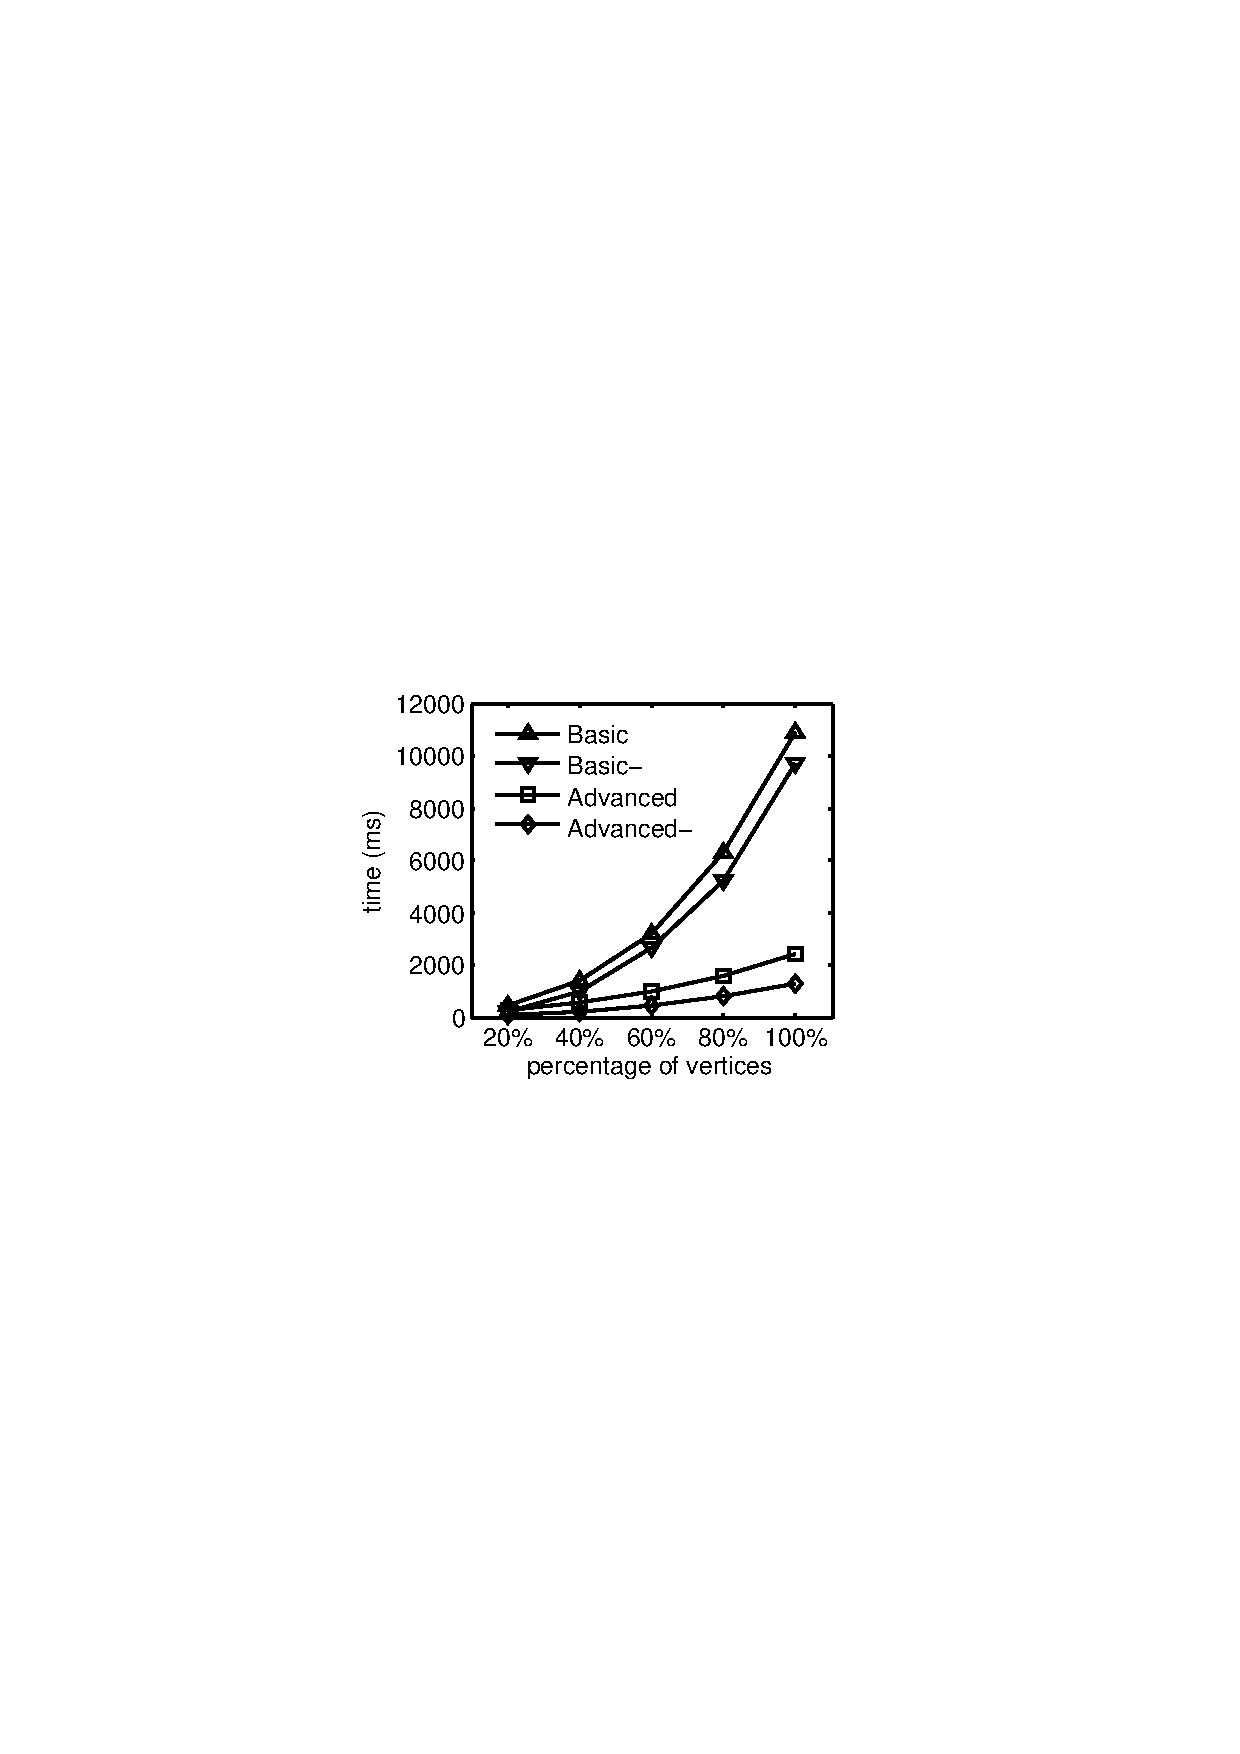
\includegraphics[width=3.725cm]{figures/flickr-index}
  \end{minipage}
  &
  \begin{minipage}{3.76cm}
	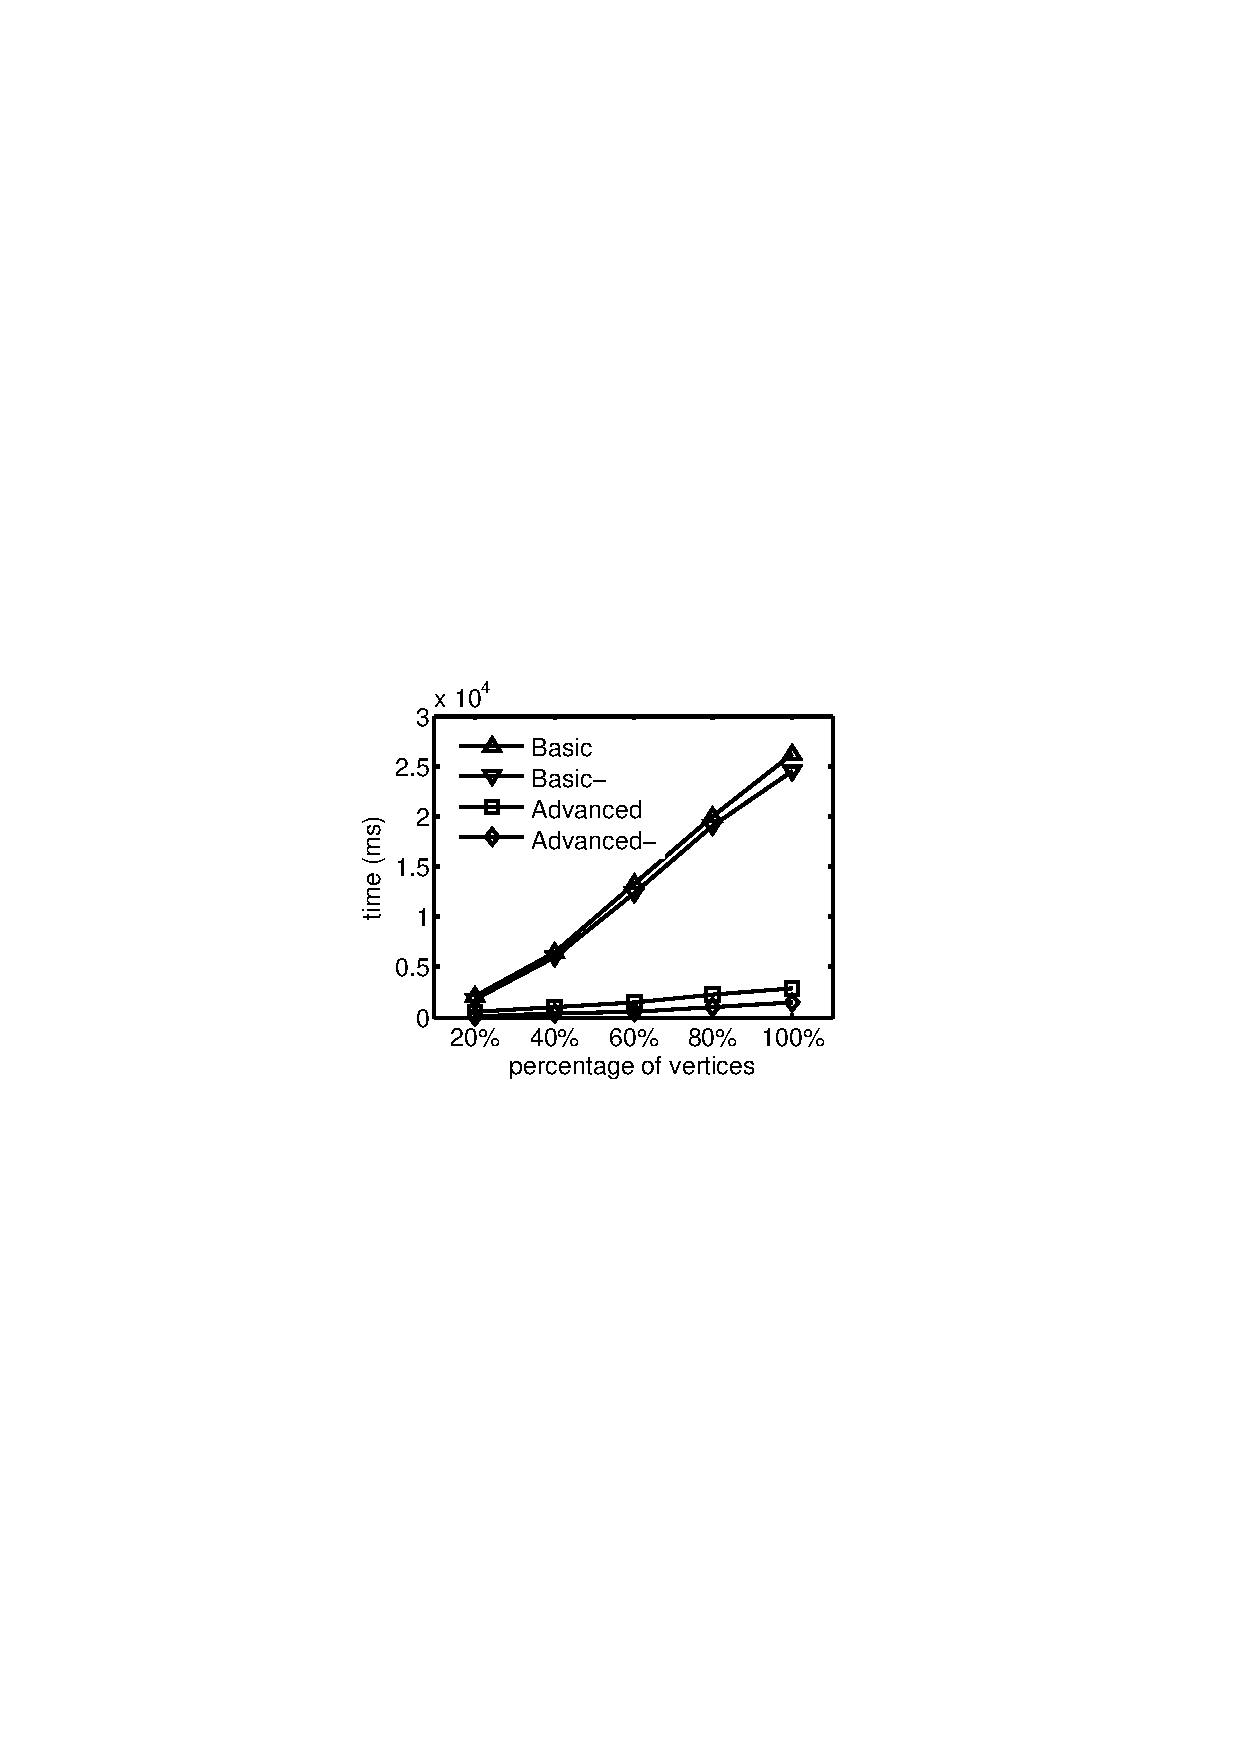
\includegraphics[width=3.725cm]{figures/dblp-index}
  \end{minipage}
  &
  \begin{minipage}{3.76cm}
	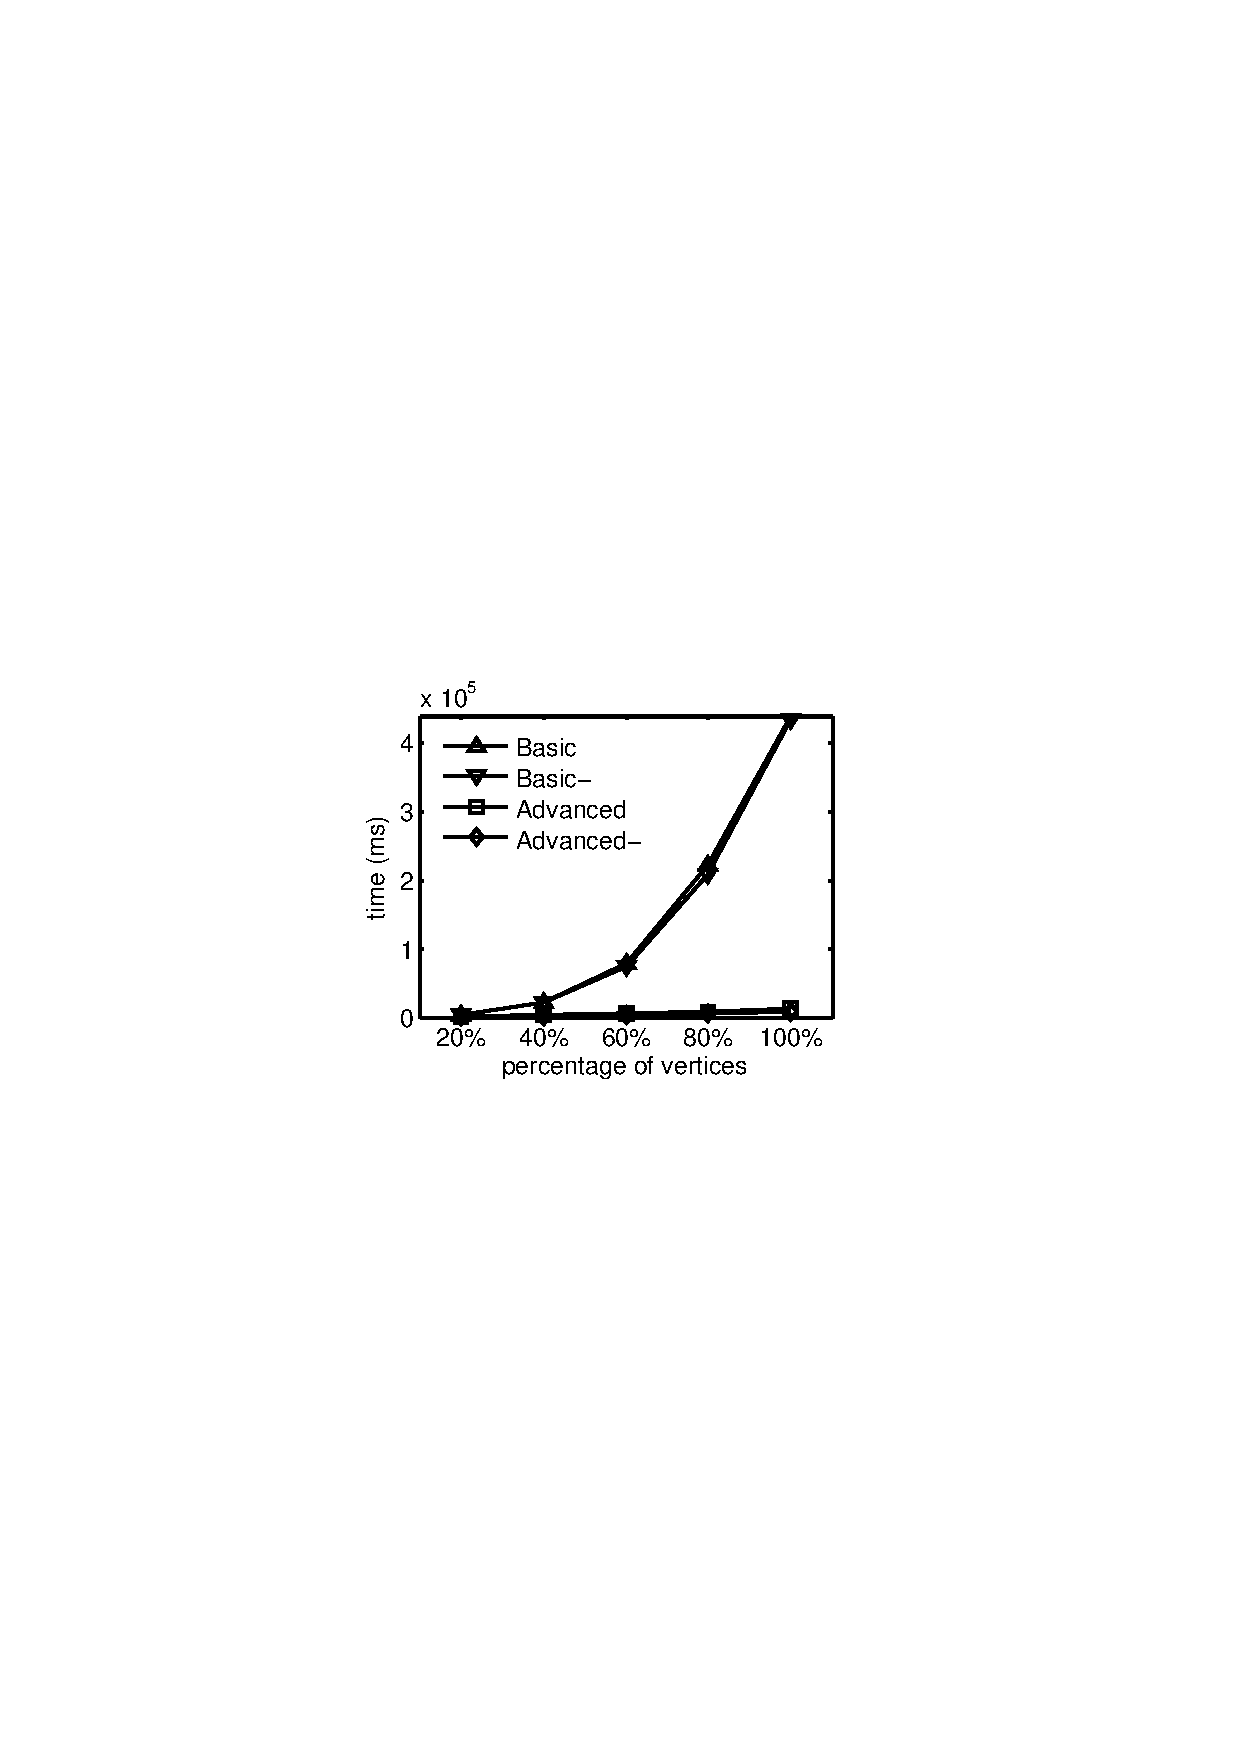
\includegraphics[width=3.725cm]{figures/tencent-index}
  \end{minipage}
  &
  \begin{minipage}{3.76cm}
	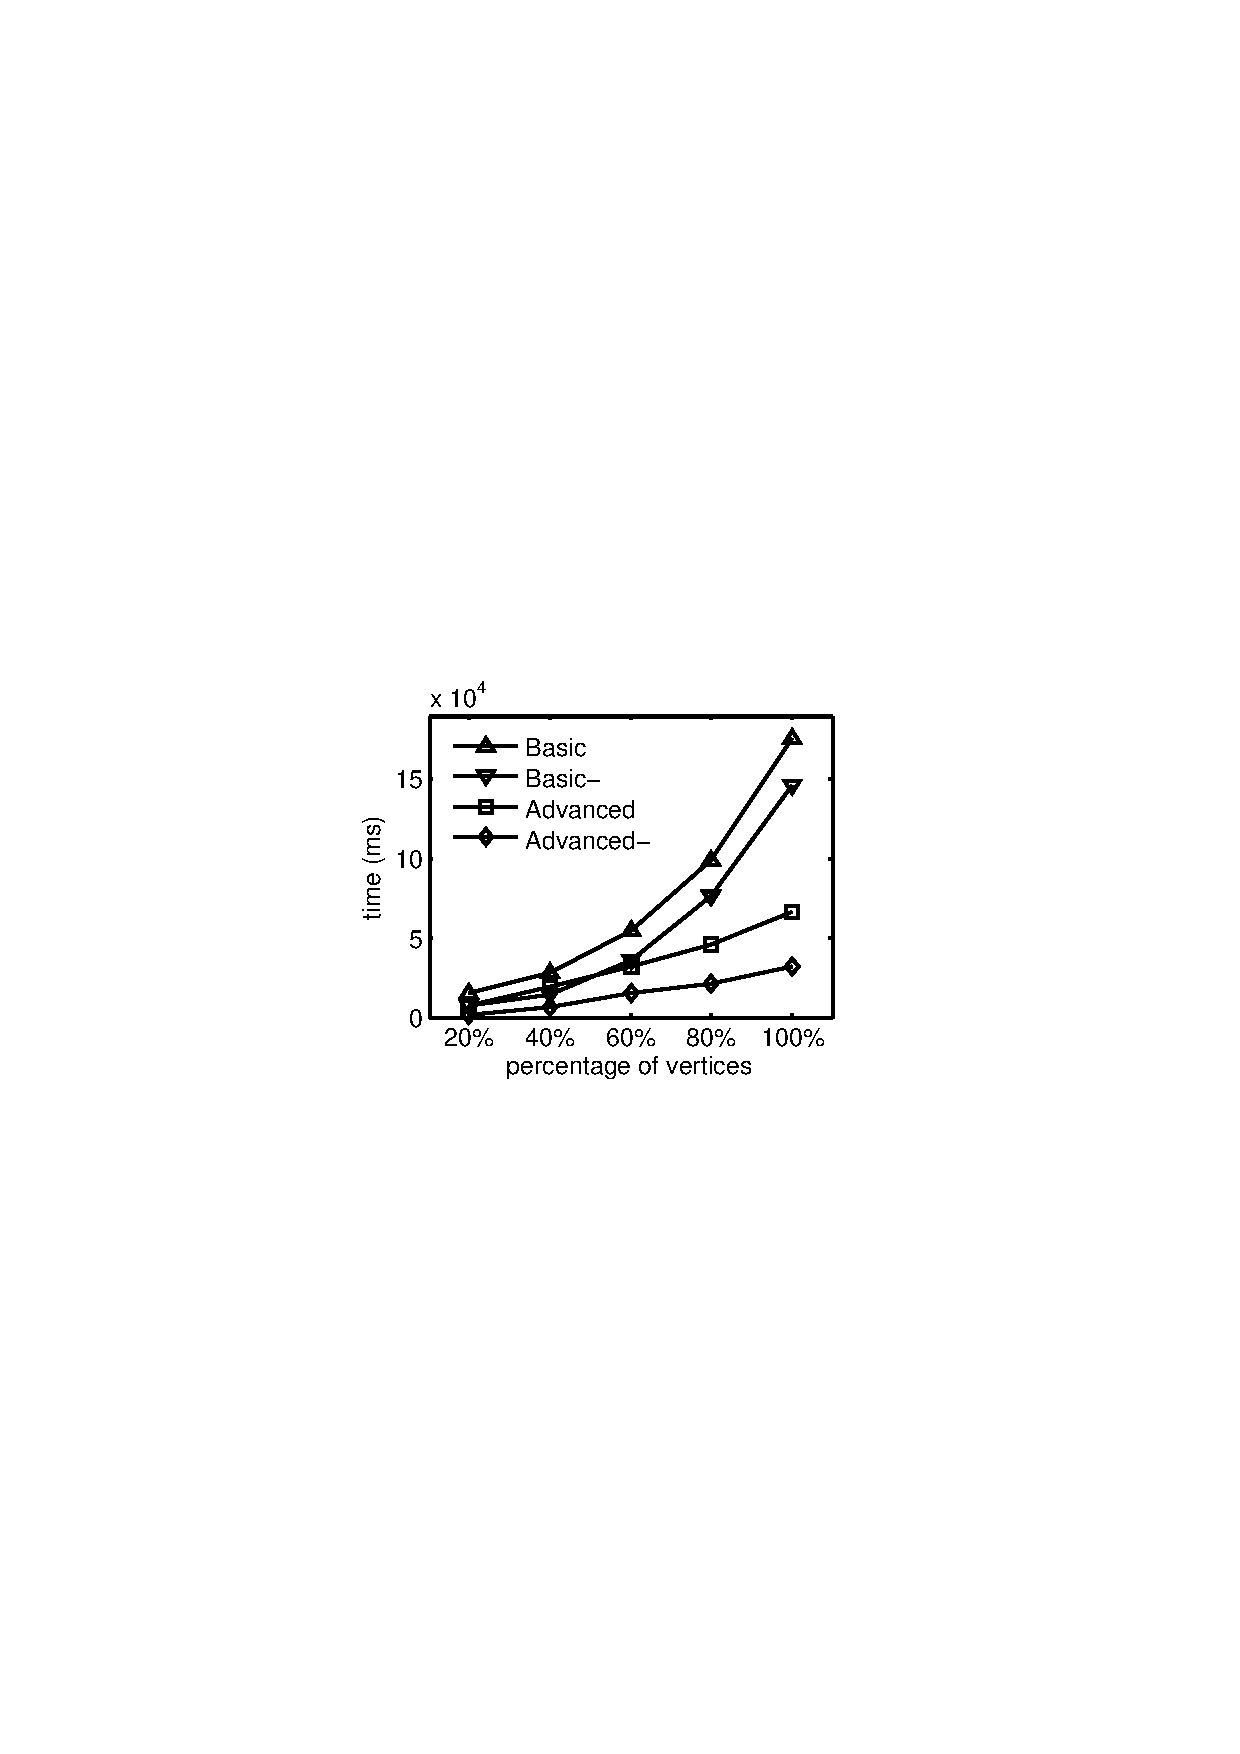
\includegraphics[width=3.725cm]{figures/dbpedia-index}
  \end{minipage}
  \\
  \small (a) Flickr (scalability)
  &
  \small (b) DBLP (scalability)
  &
  \small (c) Tencent (scalability)
  &
  \small (d) DBpedia (scalability)
\end{tabular}
\caption{Efficiency results of index construction.}
\label{fig:exp-index}
\end{figure*}



\begin{figure*}[htp]
\hspace*{-.4cm}
\centering
\begin{tabular}{c c c c}
  \begin{minipage}{3.76cm}
  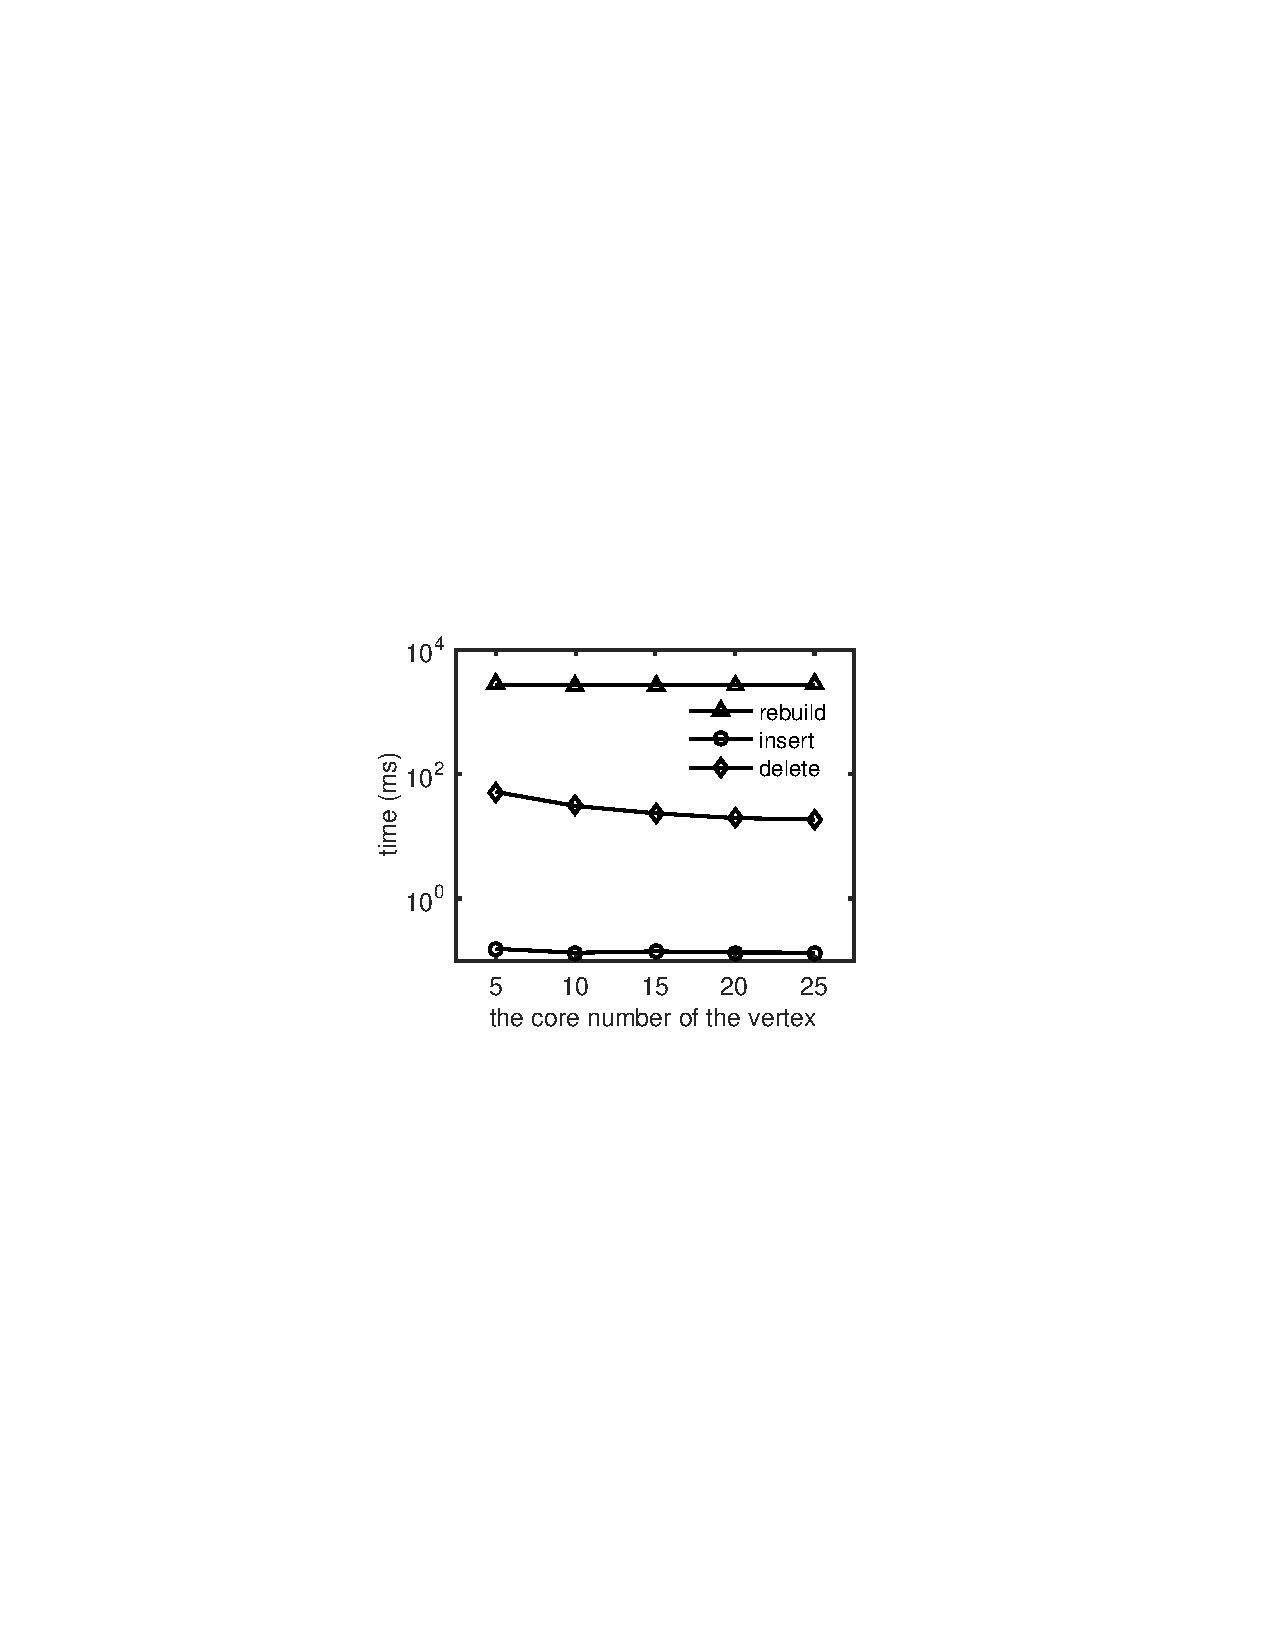
\includegraphics[width=3.725cm]{figures/flickrUpdate}
  \end{minipage}
  &
  \begin{minipage}{3.76cm}
  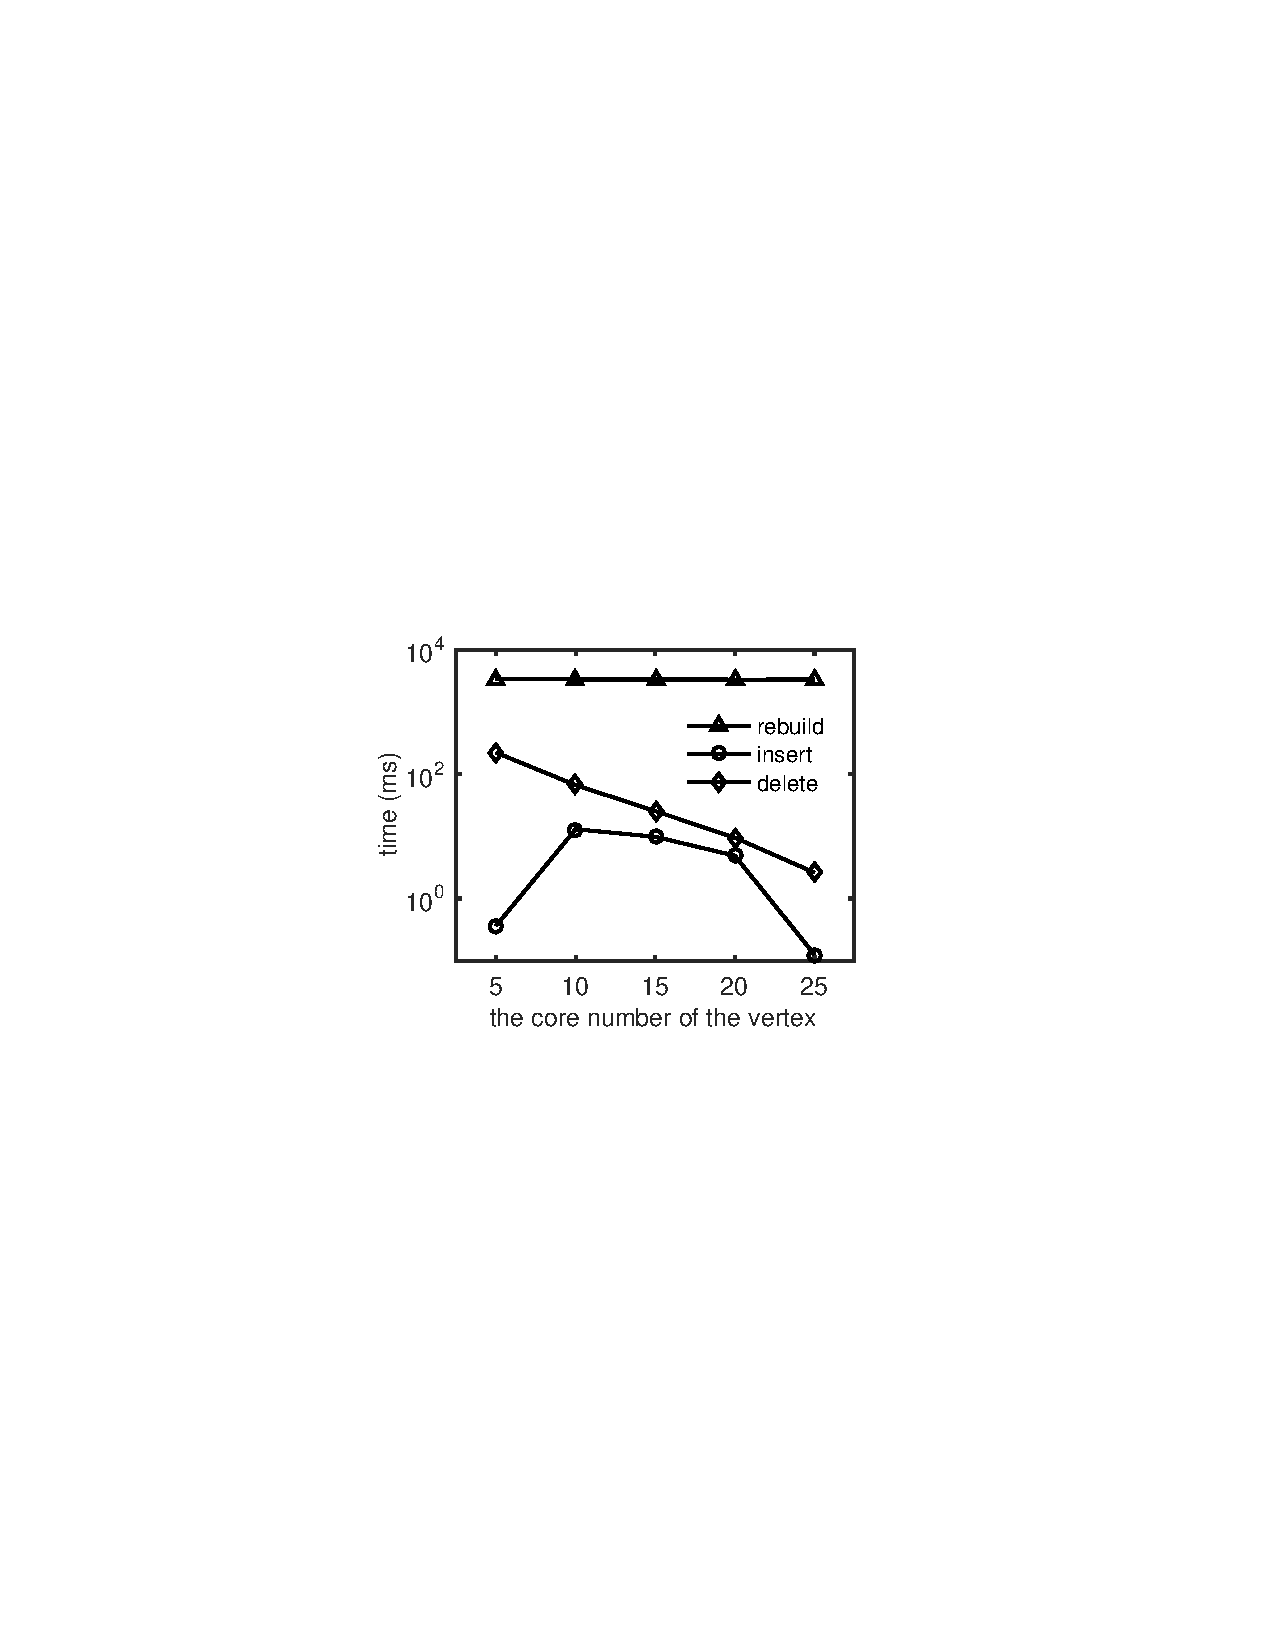
\includegraphics[width=3.725cm]{figures/dblpUpdate}
  \end{minipage}
  &
  \begin{minipage}{3.76cm}
  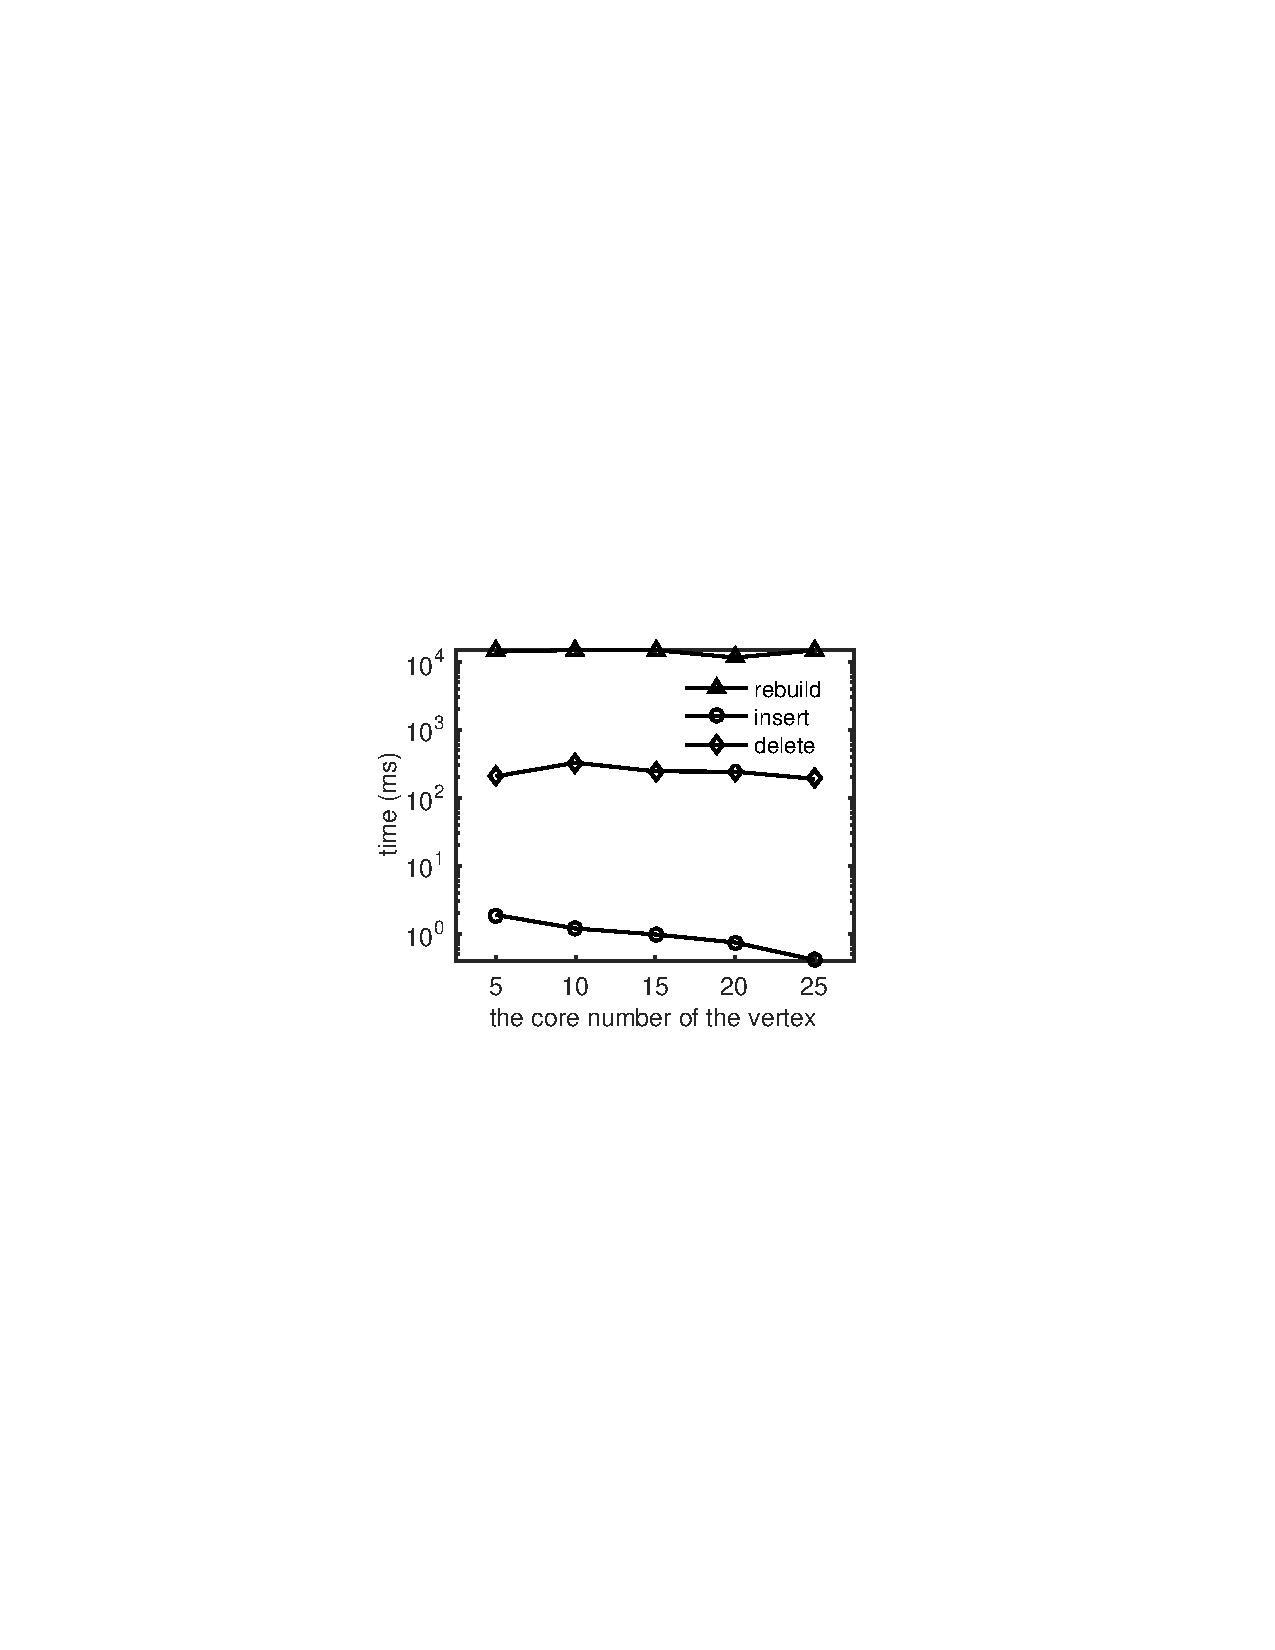
\includegraphics[width=3.725cm]{figures/tencentUpdate}
  \end{minipage}
  &
  \begin{minipage}{3.76cm}
  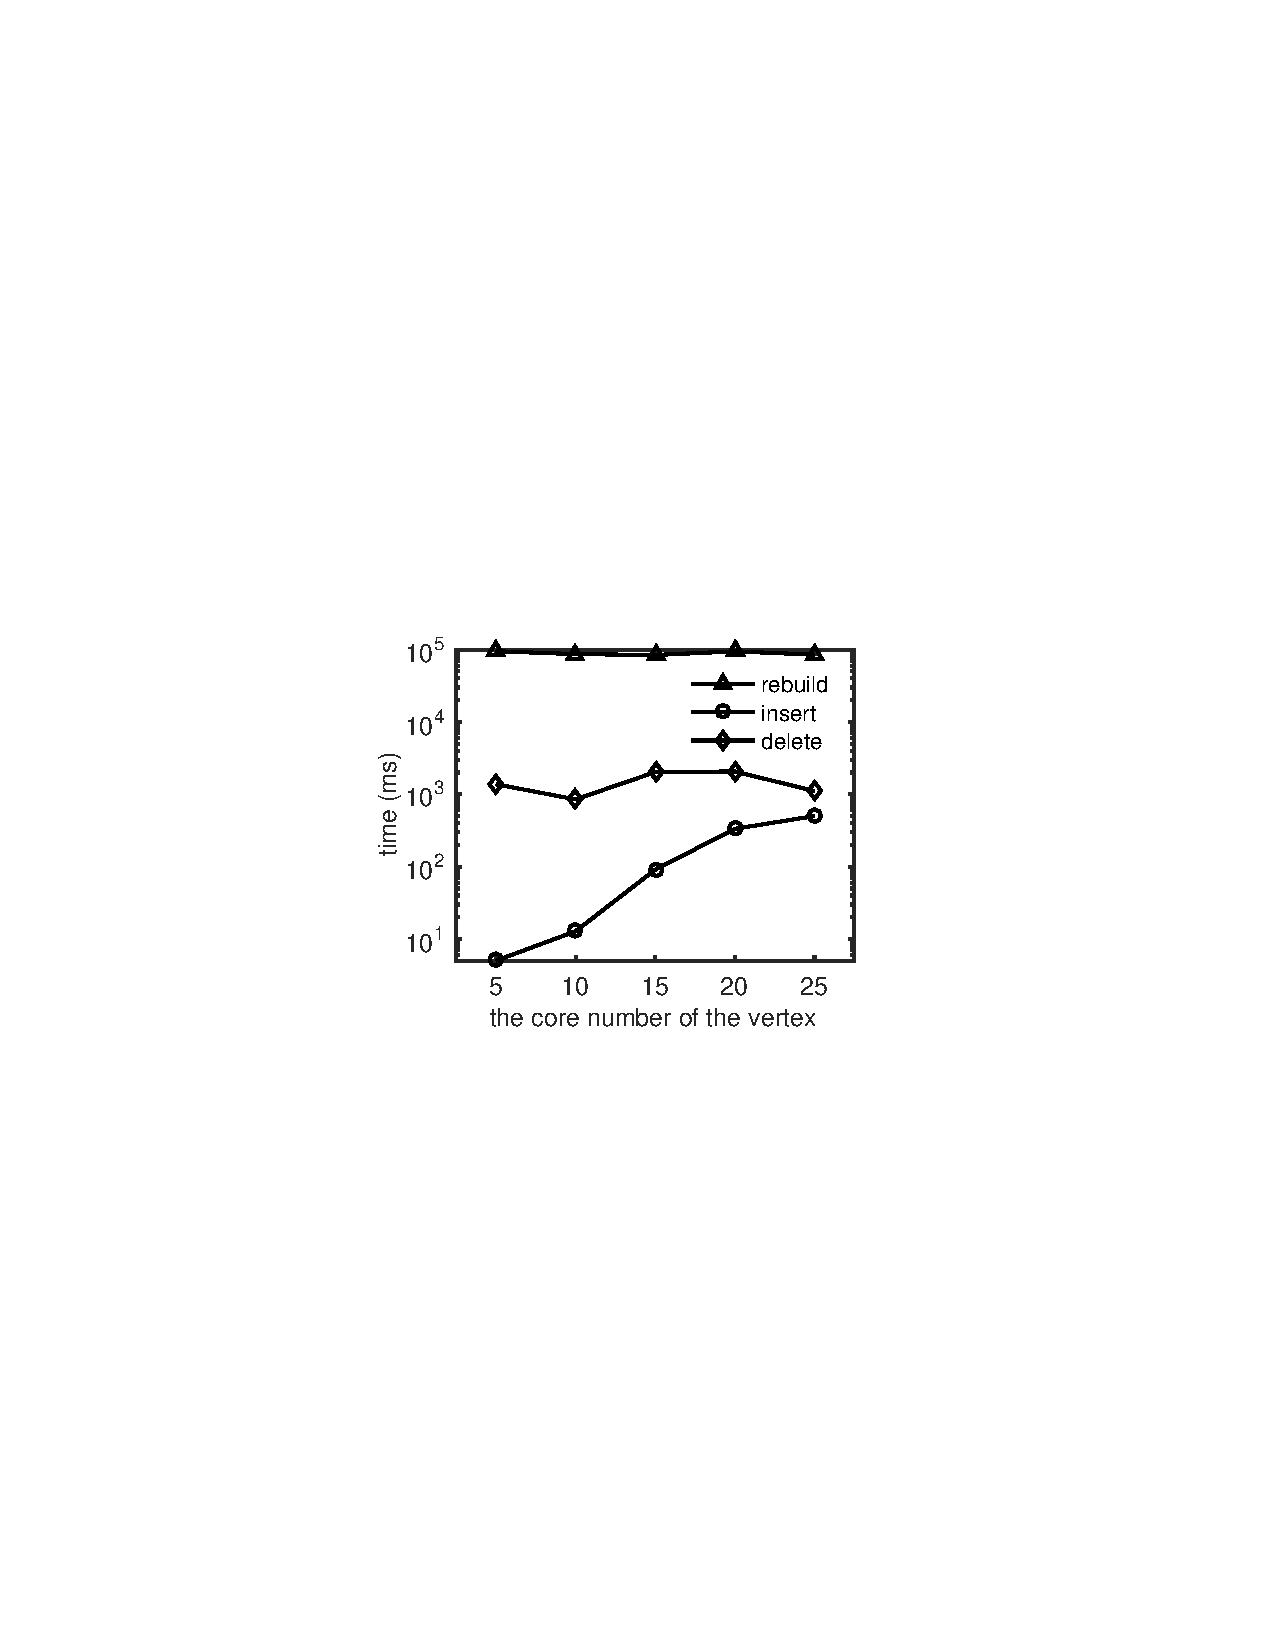
\includegraphics[width=3.725cm]{figures/dbpediaUpdate}
  \end{minipage}
  \\
  \small (a) Flickr (index maint.)
  &
  \small (b) DBLP (index maint.)
  &
  \small (c) Tencent (index maint.)
  &
  \small (d) DBpedia (index  maint.)
  \\
 \begin{minipage}{3.76cm}
  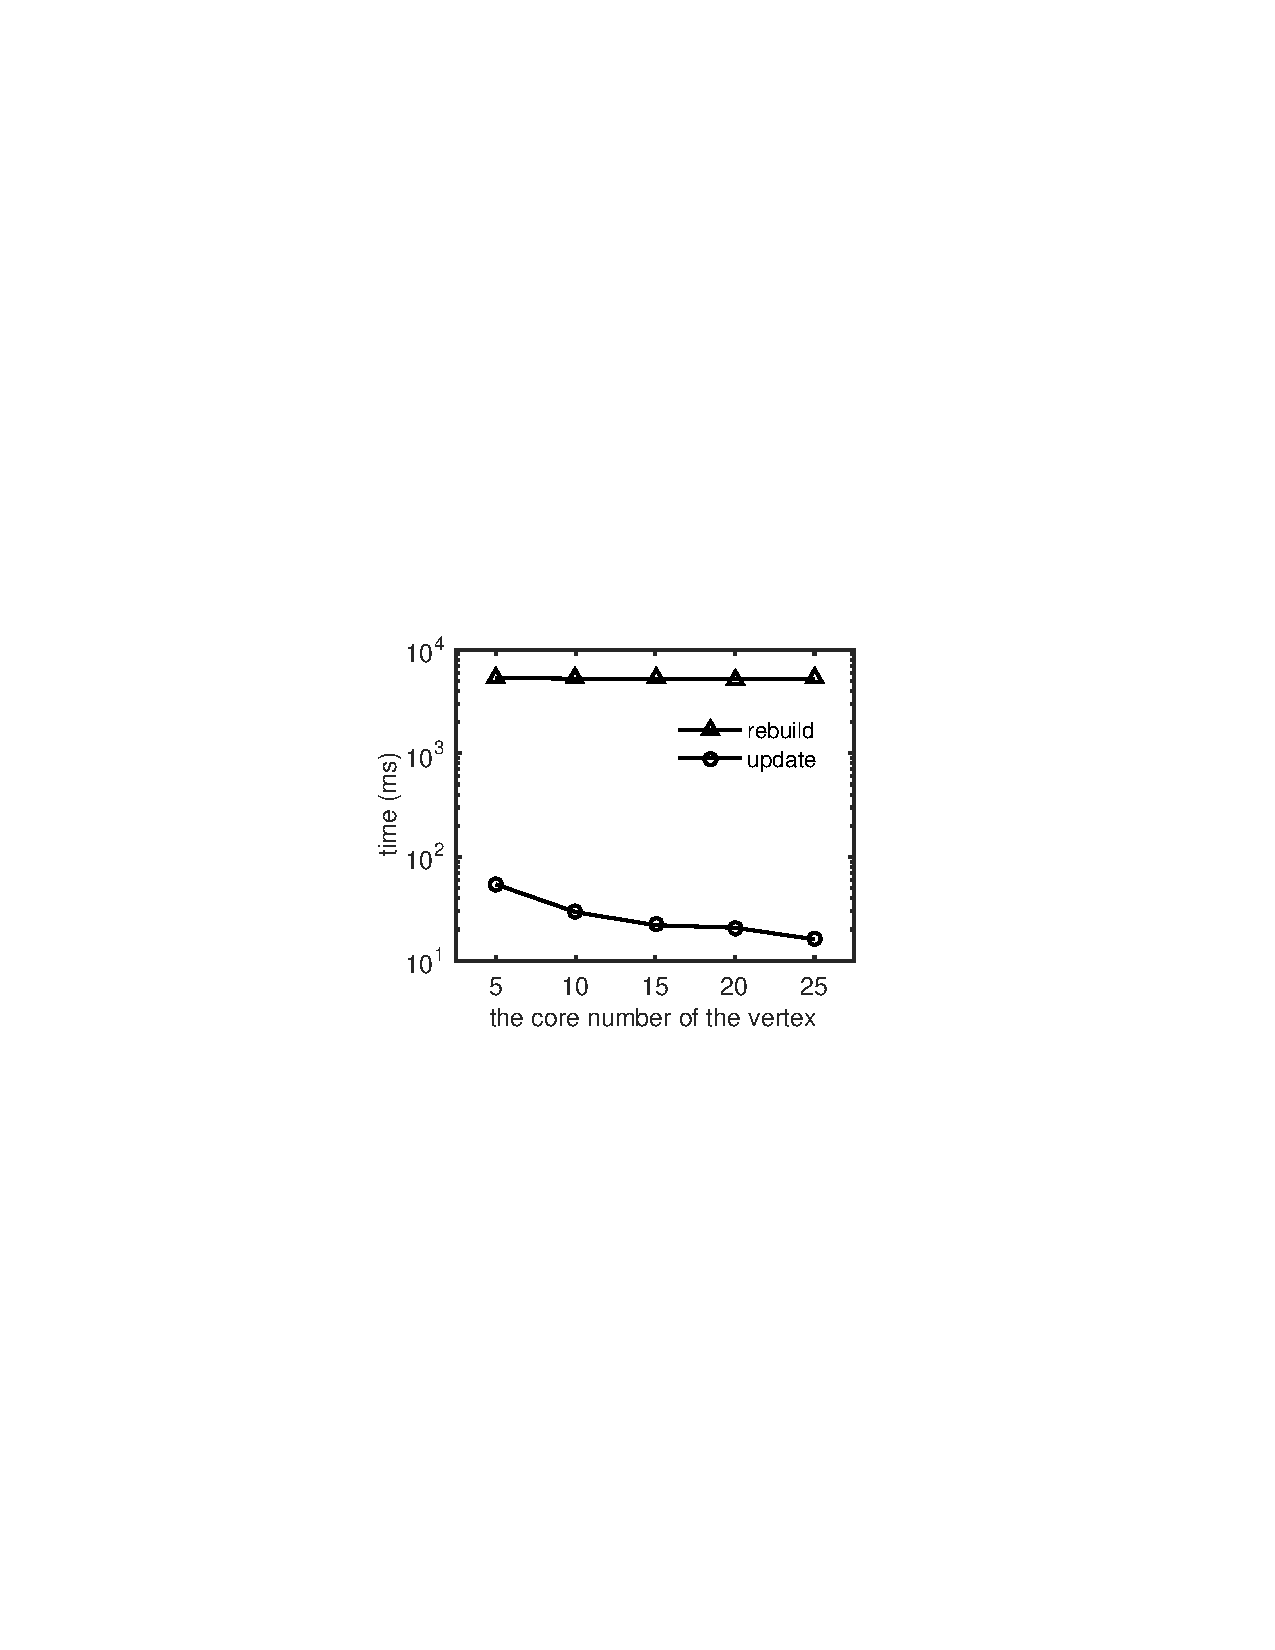
\includegraphics[width=3.725cm]{figures/flickrMix}
  \end{minipage}
  &
  \begin{minipage}{3.76cm}
  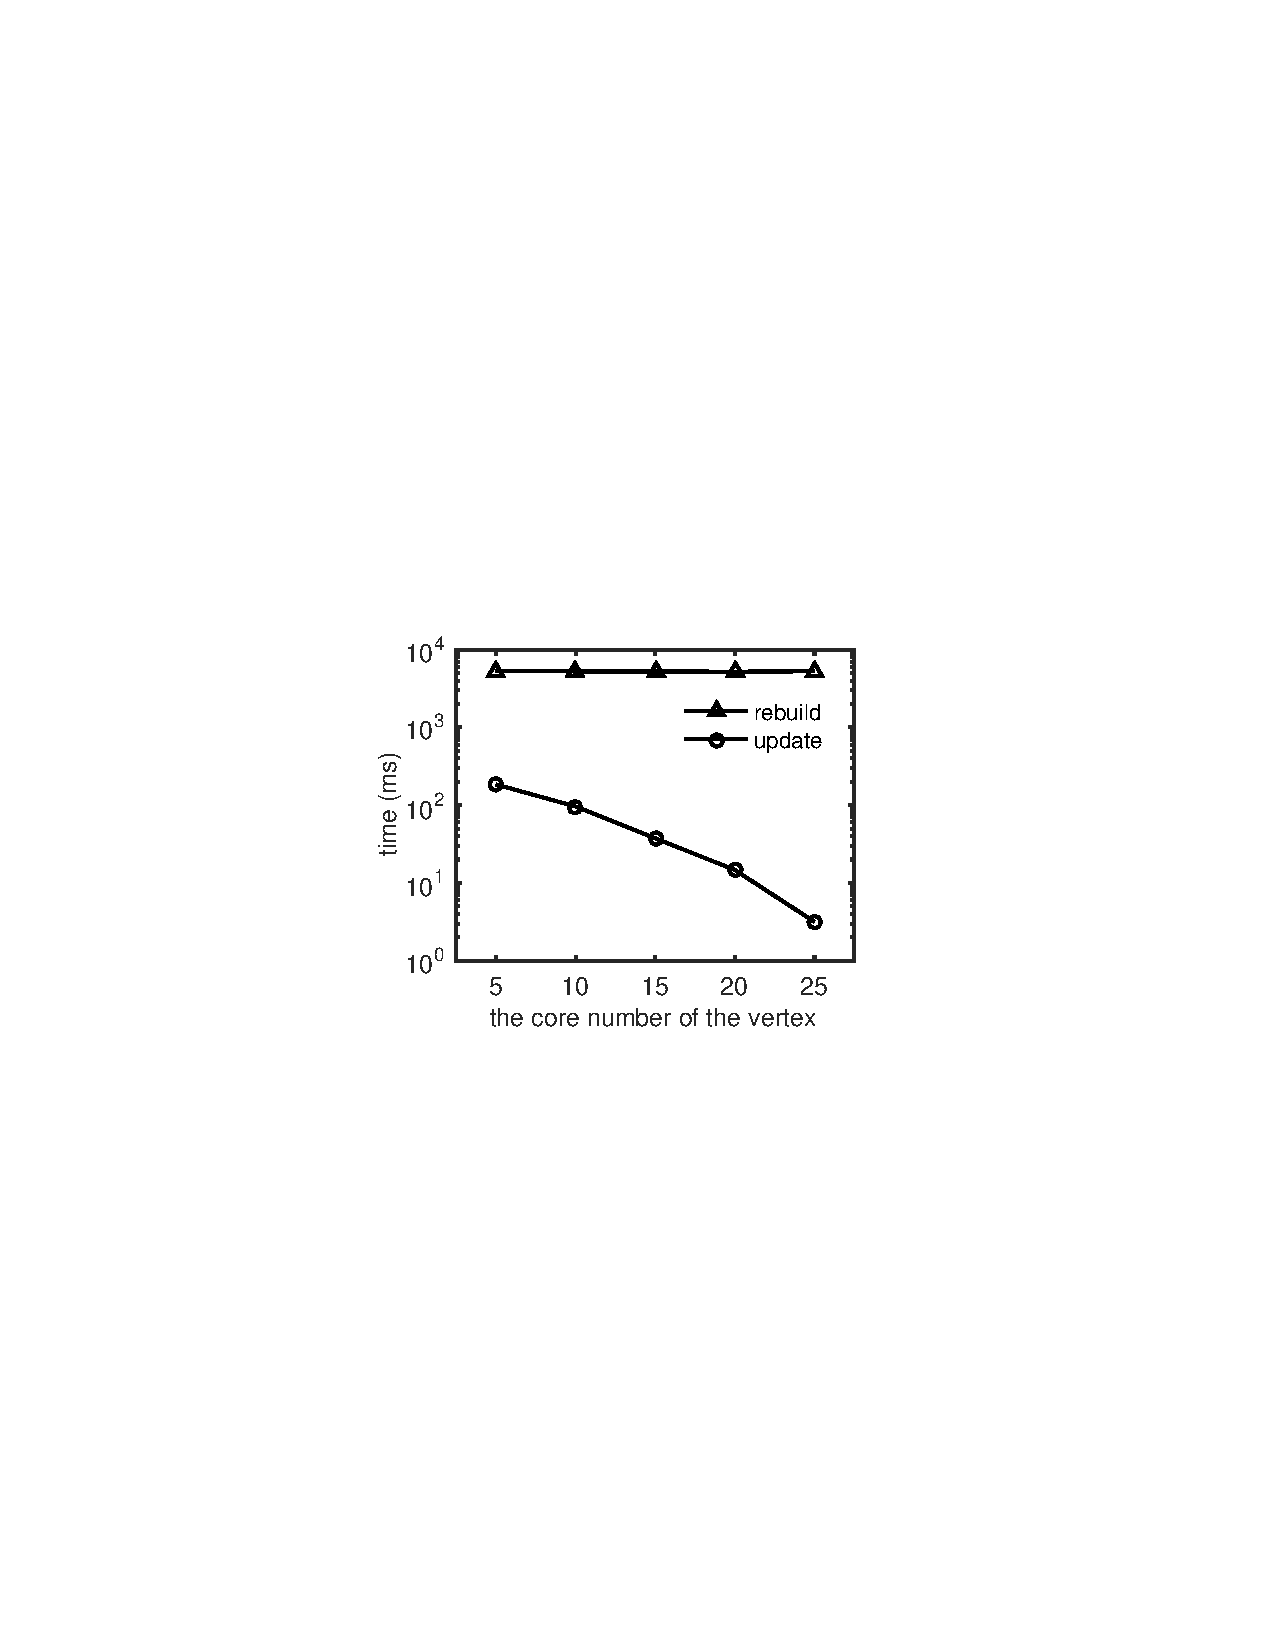
\includegraphics[width=3.725cm]{figures/dblpMix}
  \end{minipage}
  &
  \begin{minipage}{3.76cm}
  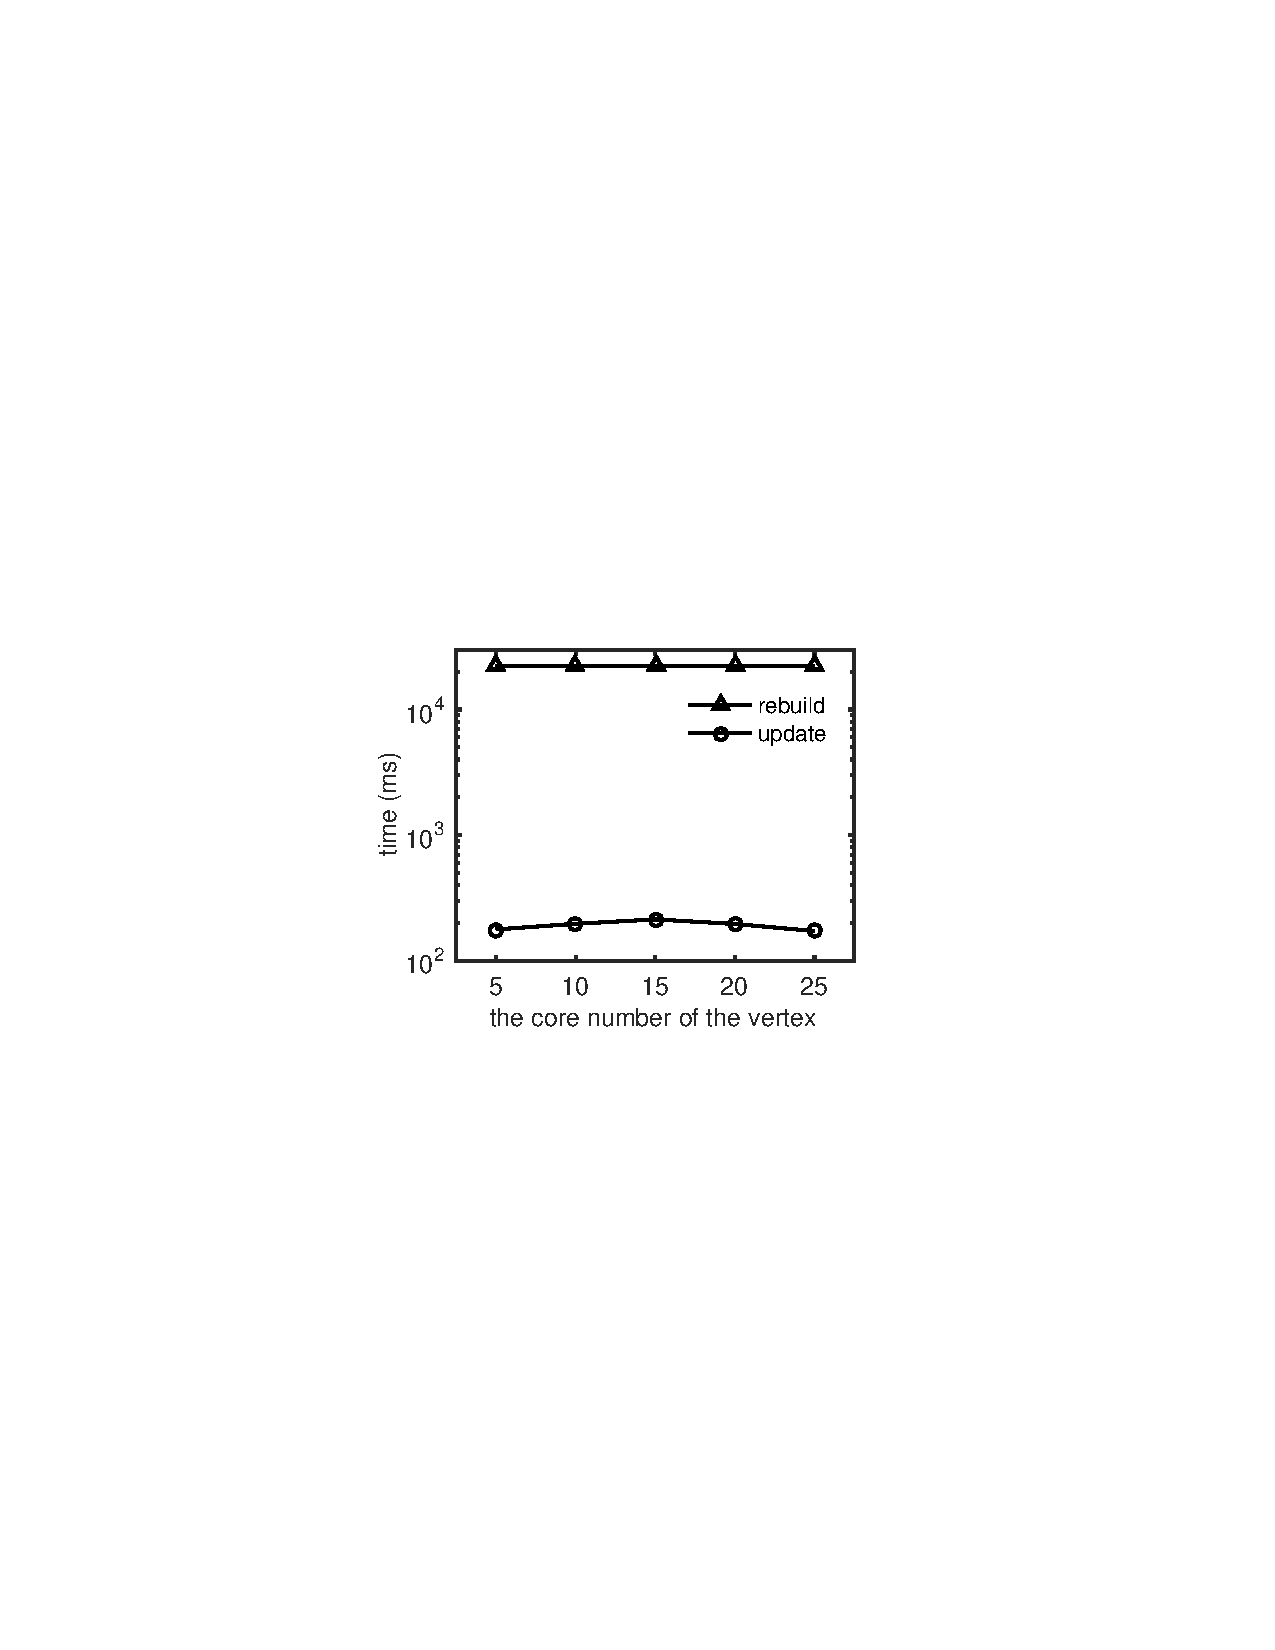
\includegraphics[width=3.725cm]{figures/tencentMix}
  \end{minipage}
  &
  \begin{minipage}{3.76cm}
  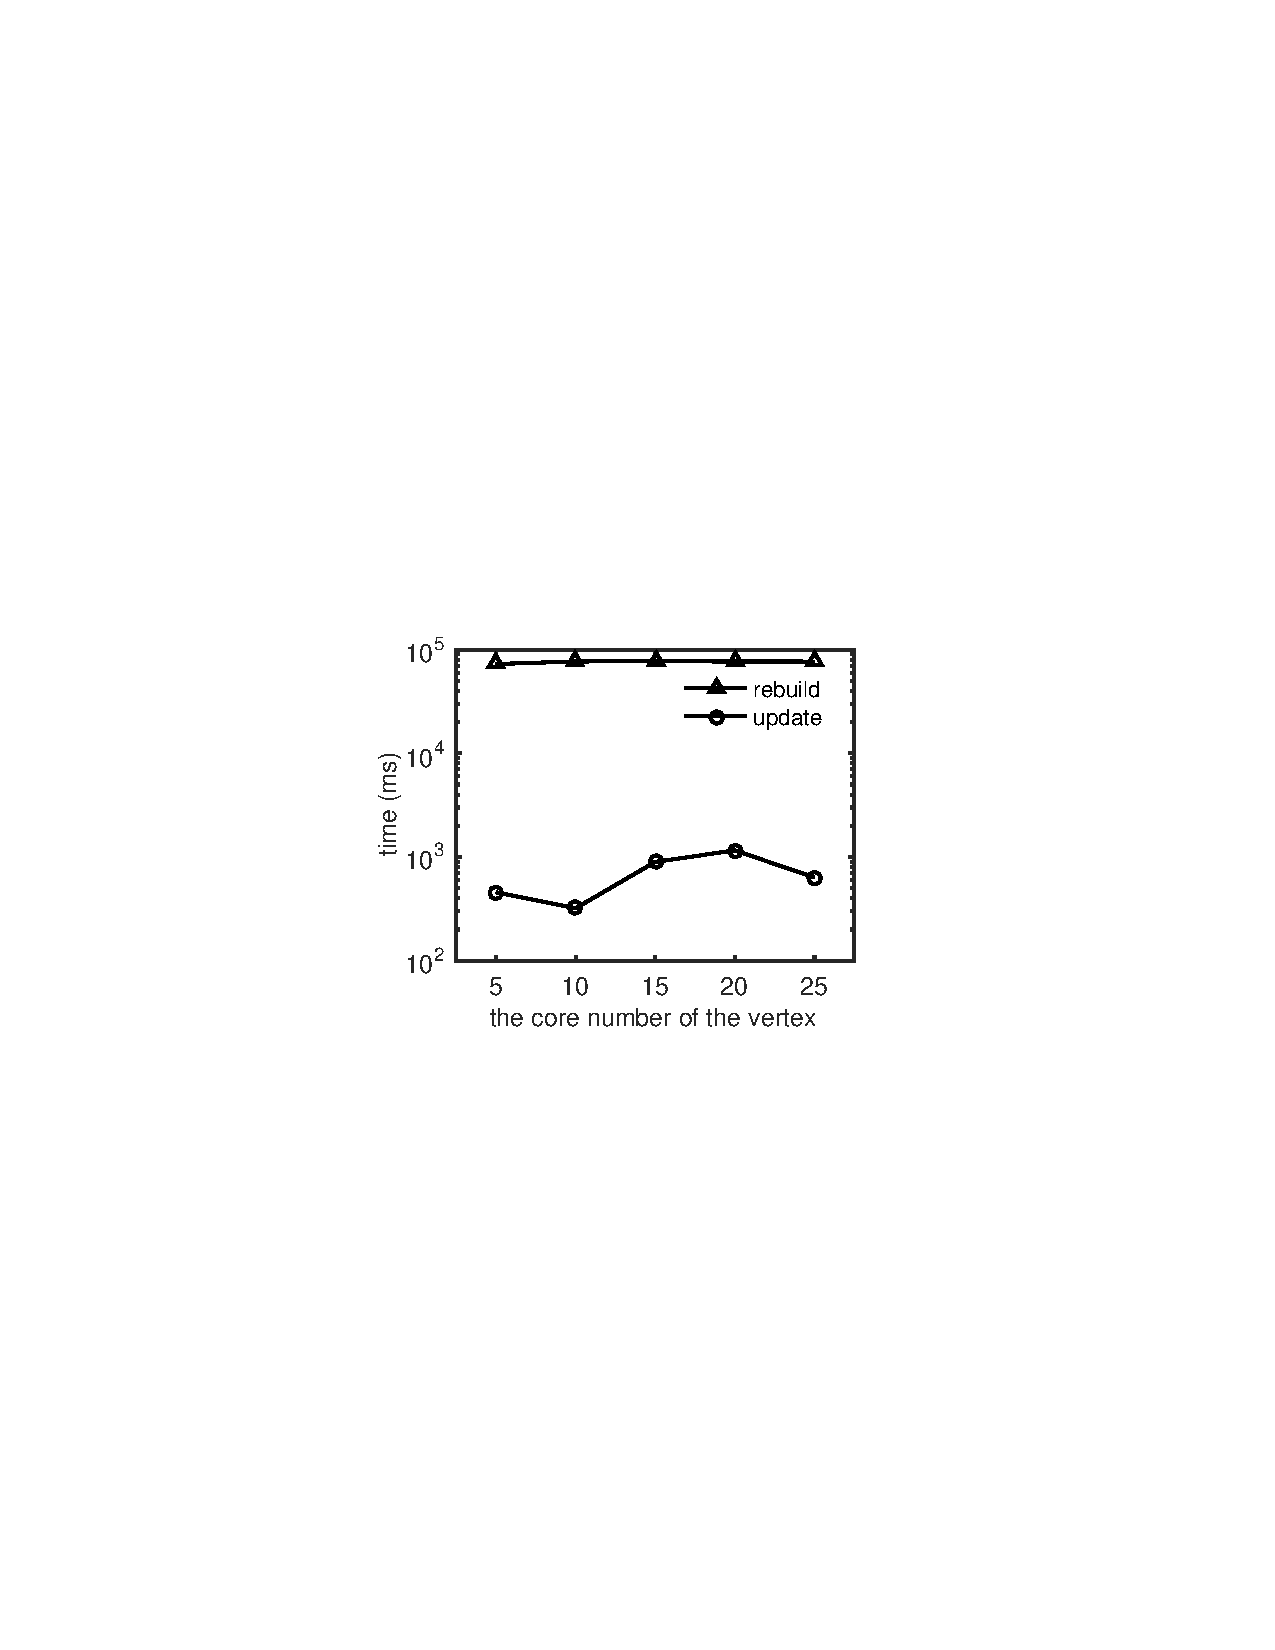
\includegraphics[width=3.725cm]{figures/dbpediaMix}
  \end{minipage}
  \\
  \small (e) Flickr (index maint.)
  &
  \small (f) DBLP (index maint.)
  &
  \small (g) Tencent (index maint.)
  &
  \small (h) DBpedia (index  maint.)
  \\
  &
 \begin{minipage}{3.325cm}
  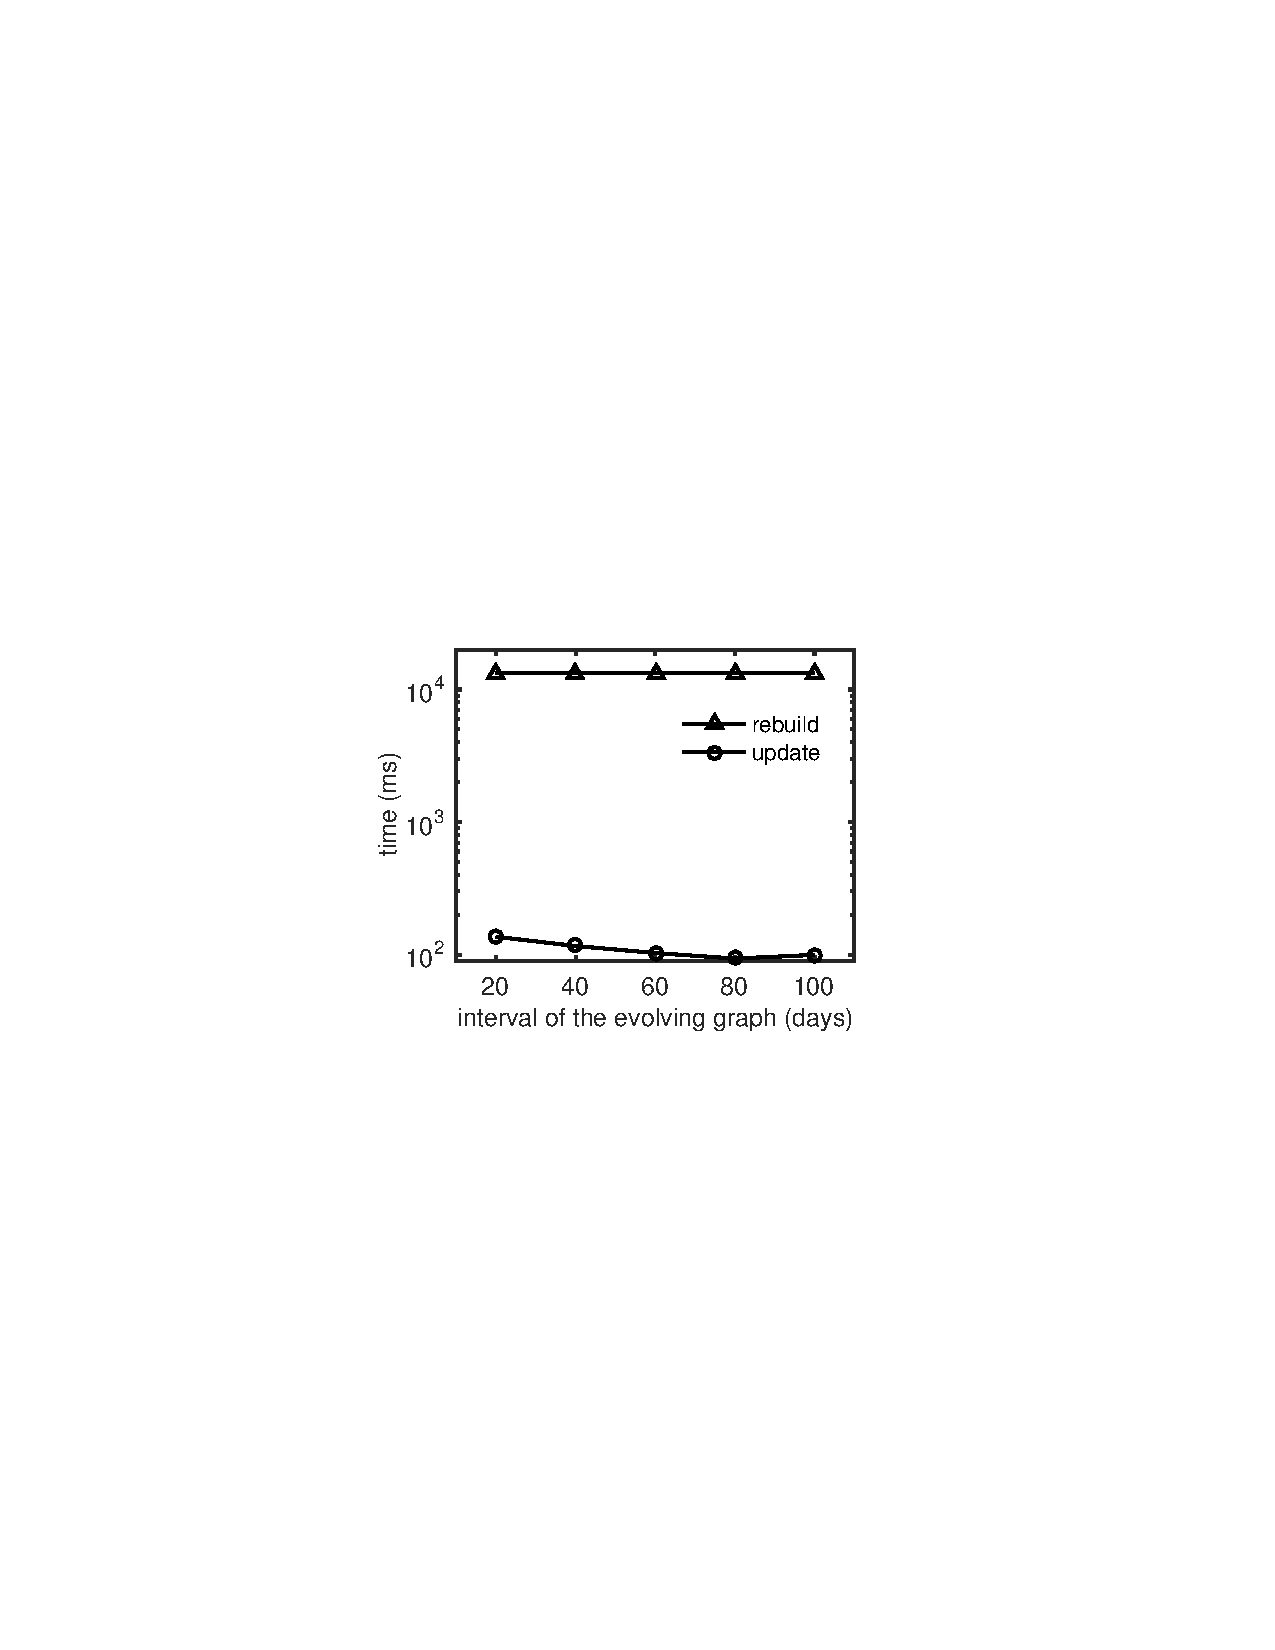
\includegraphics[width=3.725cm]{figures/DynamicFlickr}
  \end{minipage}
  &
  \begin{minipage}{3.325cm}
  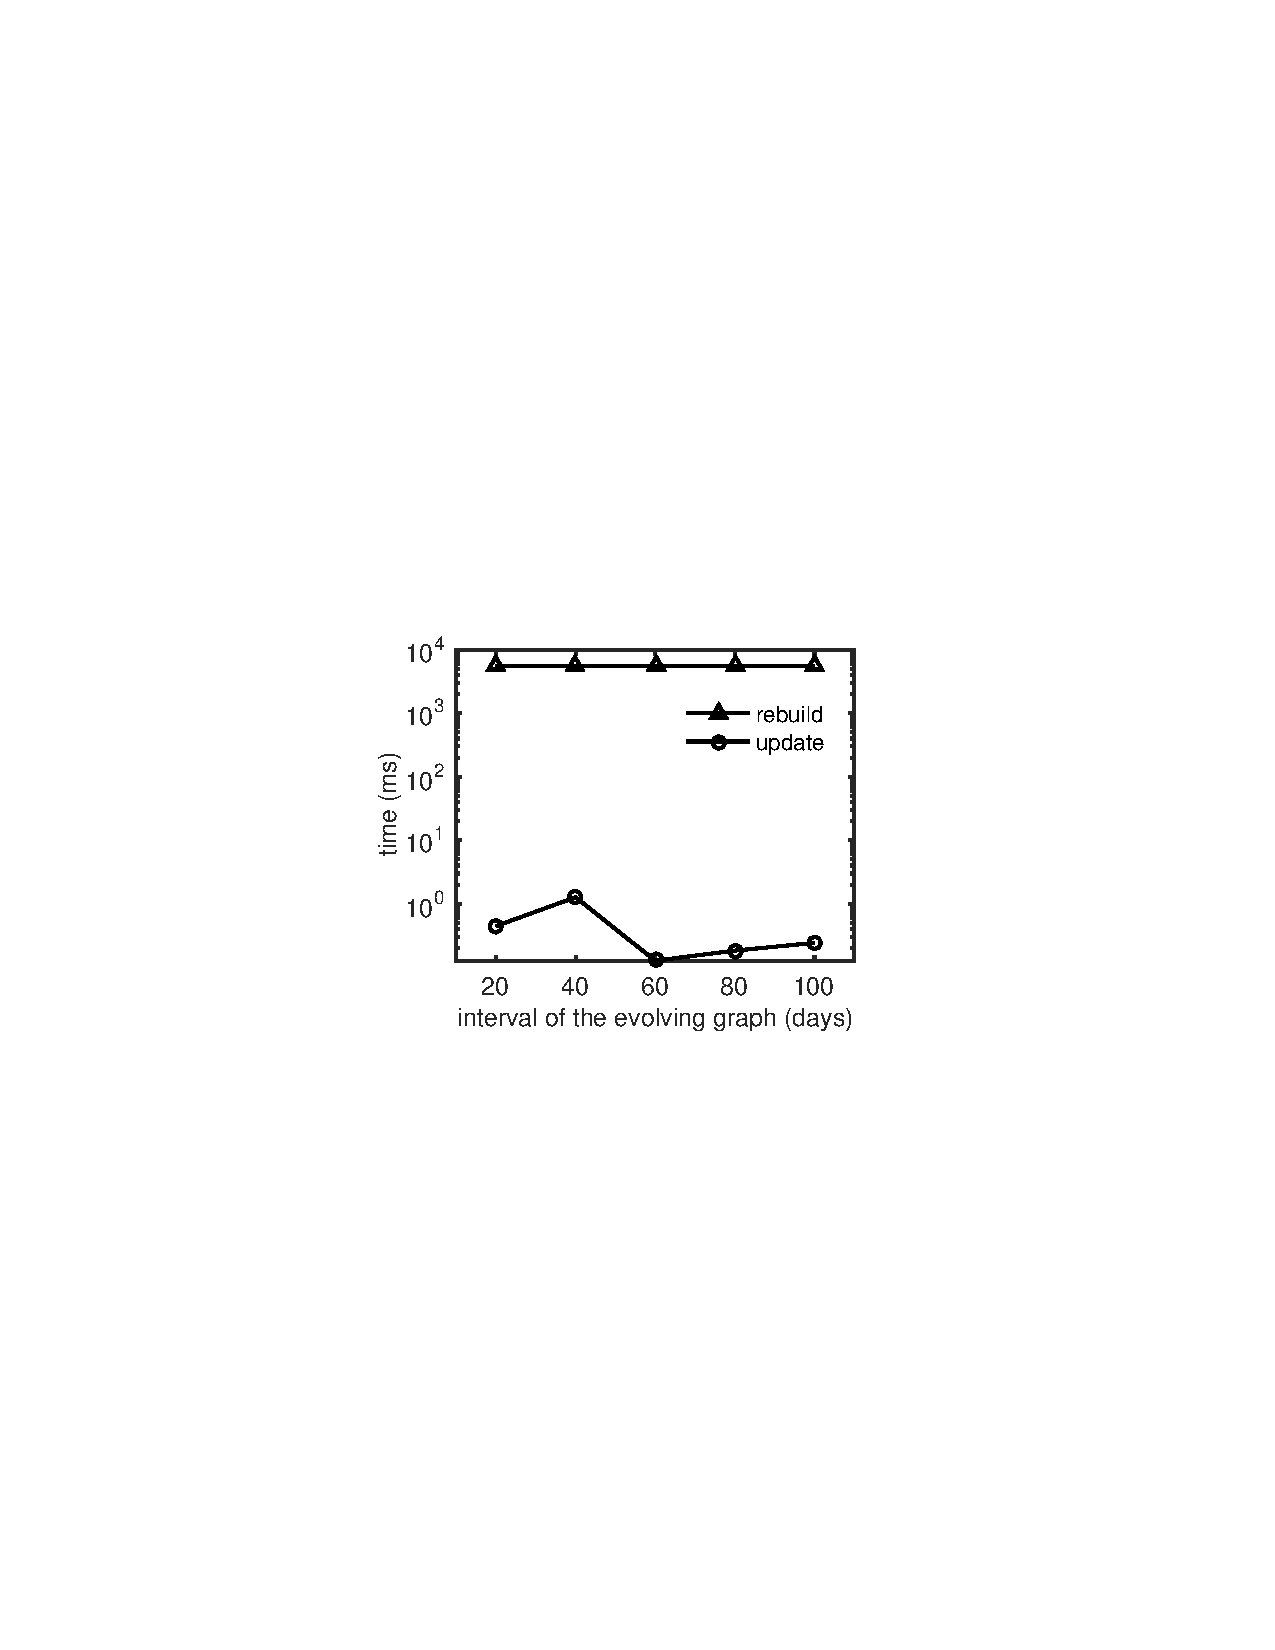
\includegraphics[width=3.725cm]{figures/DynamicYoutube}
  \end{minipage}
  \\
  &
  \small (i) DFlickr
  &
  \small (j) Youtube
  &
\\
\end{tabular}
\caption{Efficiency results of index maintenance.}
\label{fig:exp-indexMaintenance}
\end{figure*}


\begin{figure*}[htp]
\hspace*{-.4cm}
\centering
\begin{tabular}{c c c c}
      \begin{minipage}{3.725cm}
	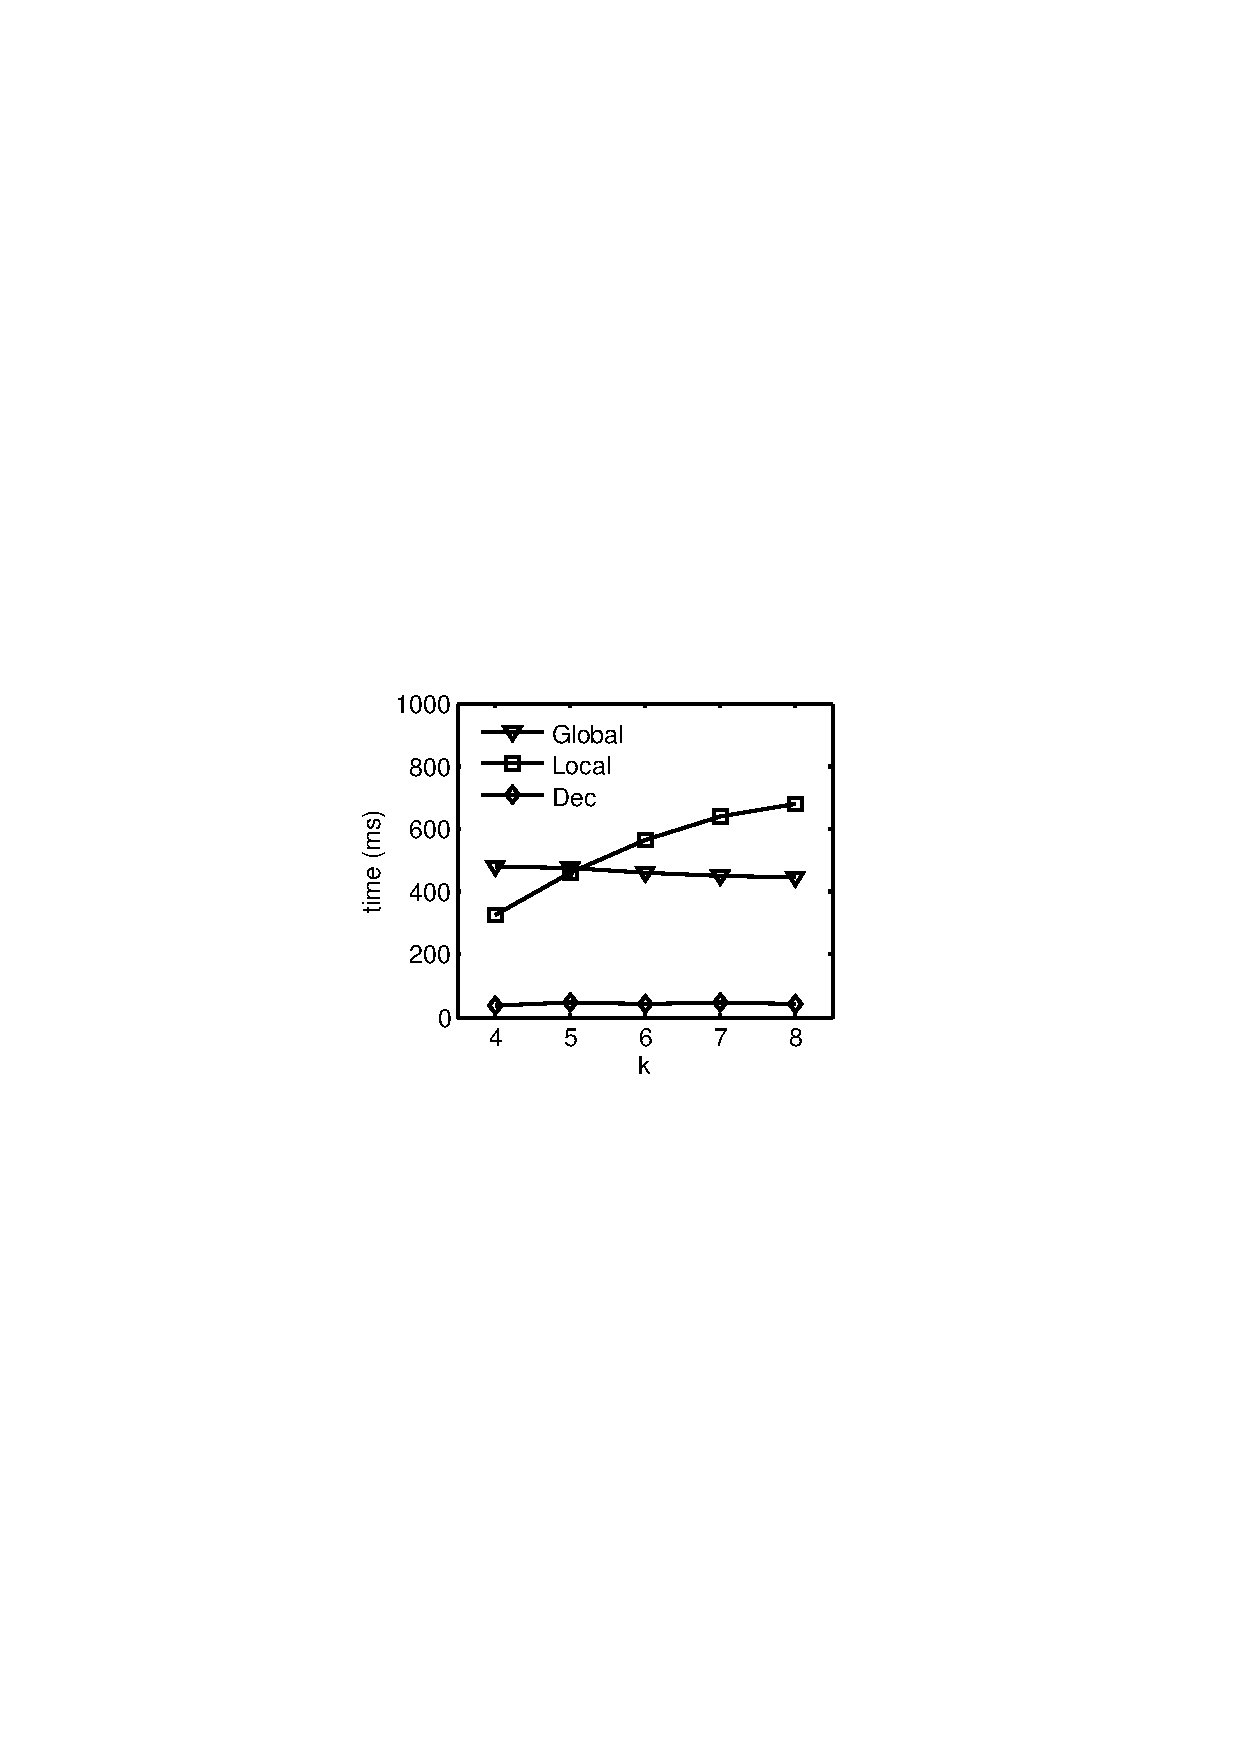
\includegraphics[width=3.725cm]{figures/flickr-comp}
  \end{minipage}
  &
  \begin{minipage}{3.725cm}
	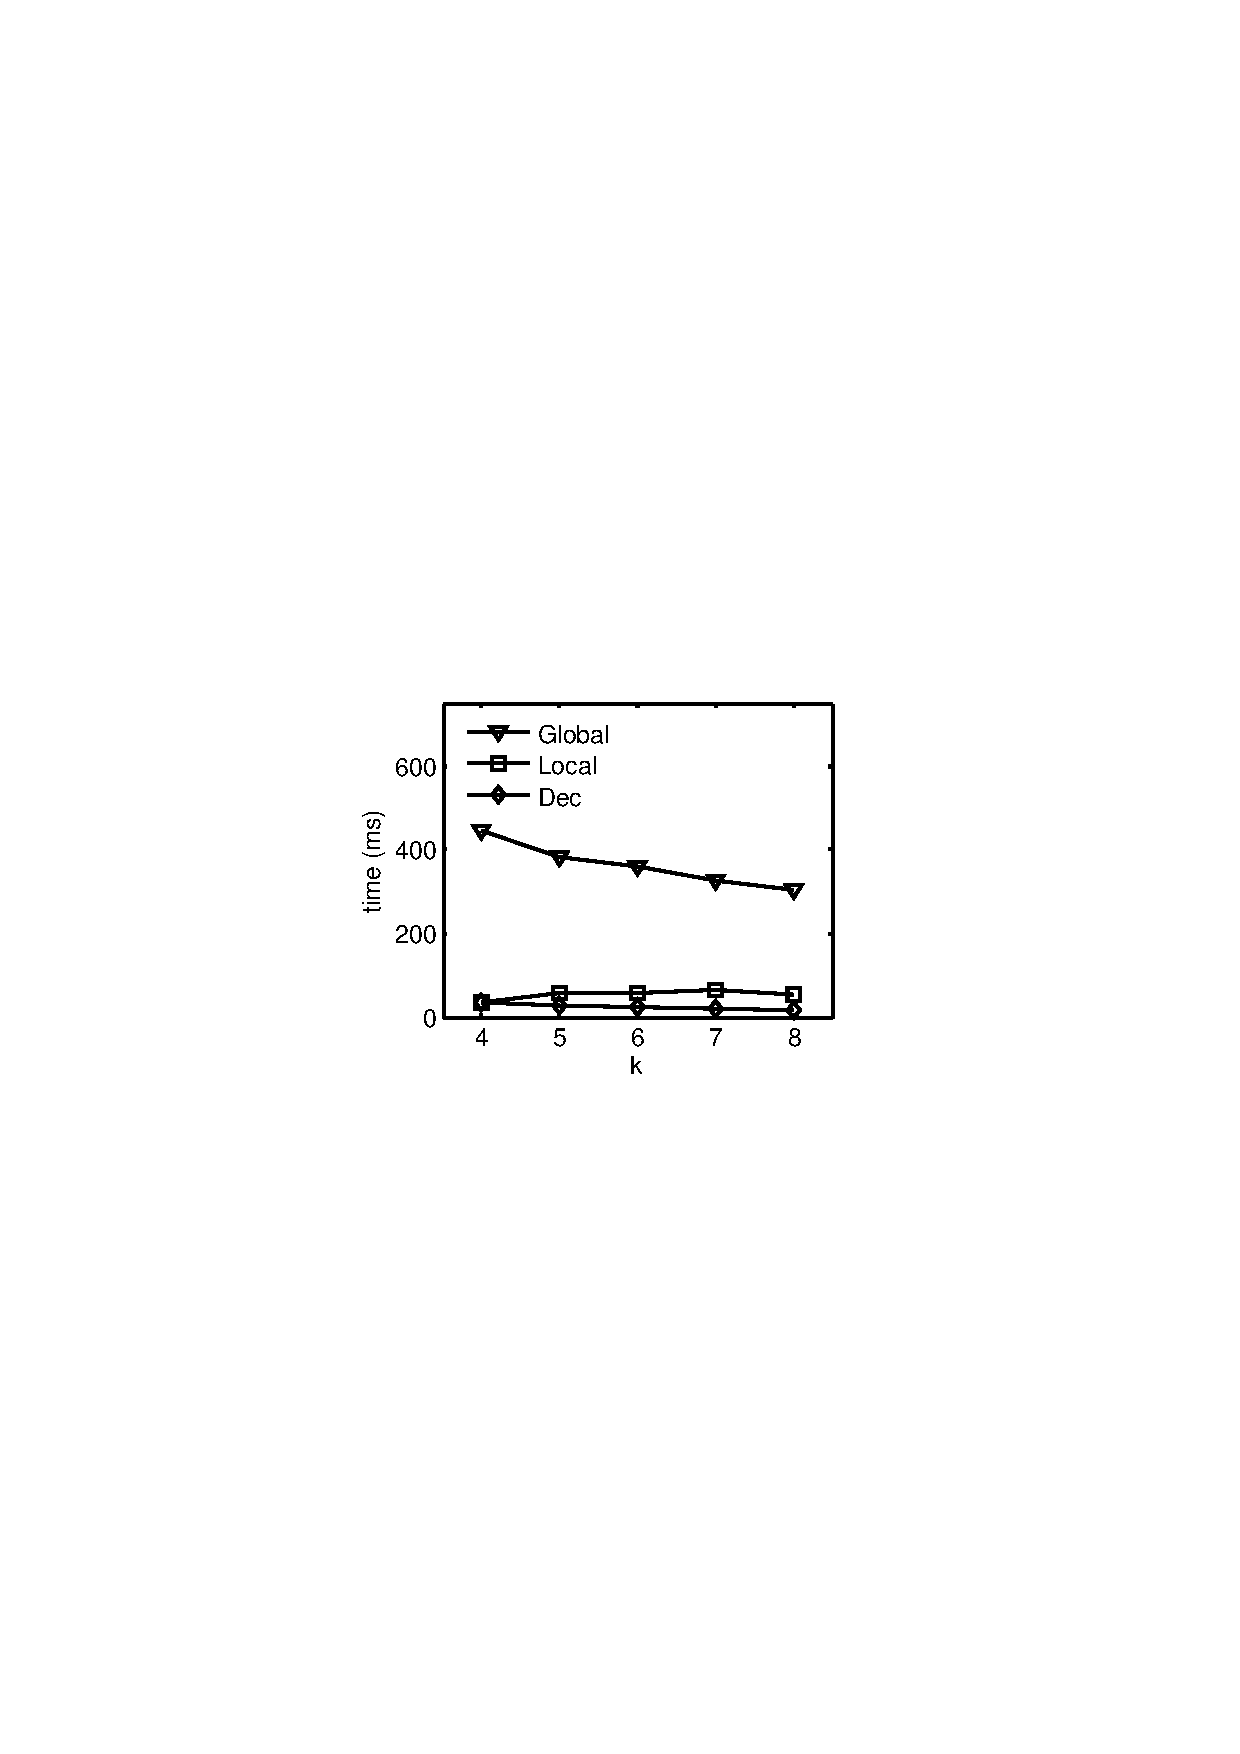
\includegraphics[width=3.725cm]{figures/dblp-comp}
  \end{minipage}
  &
  \begin{minipage}{3.725cm}
	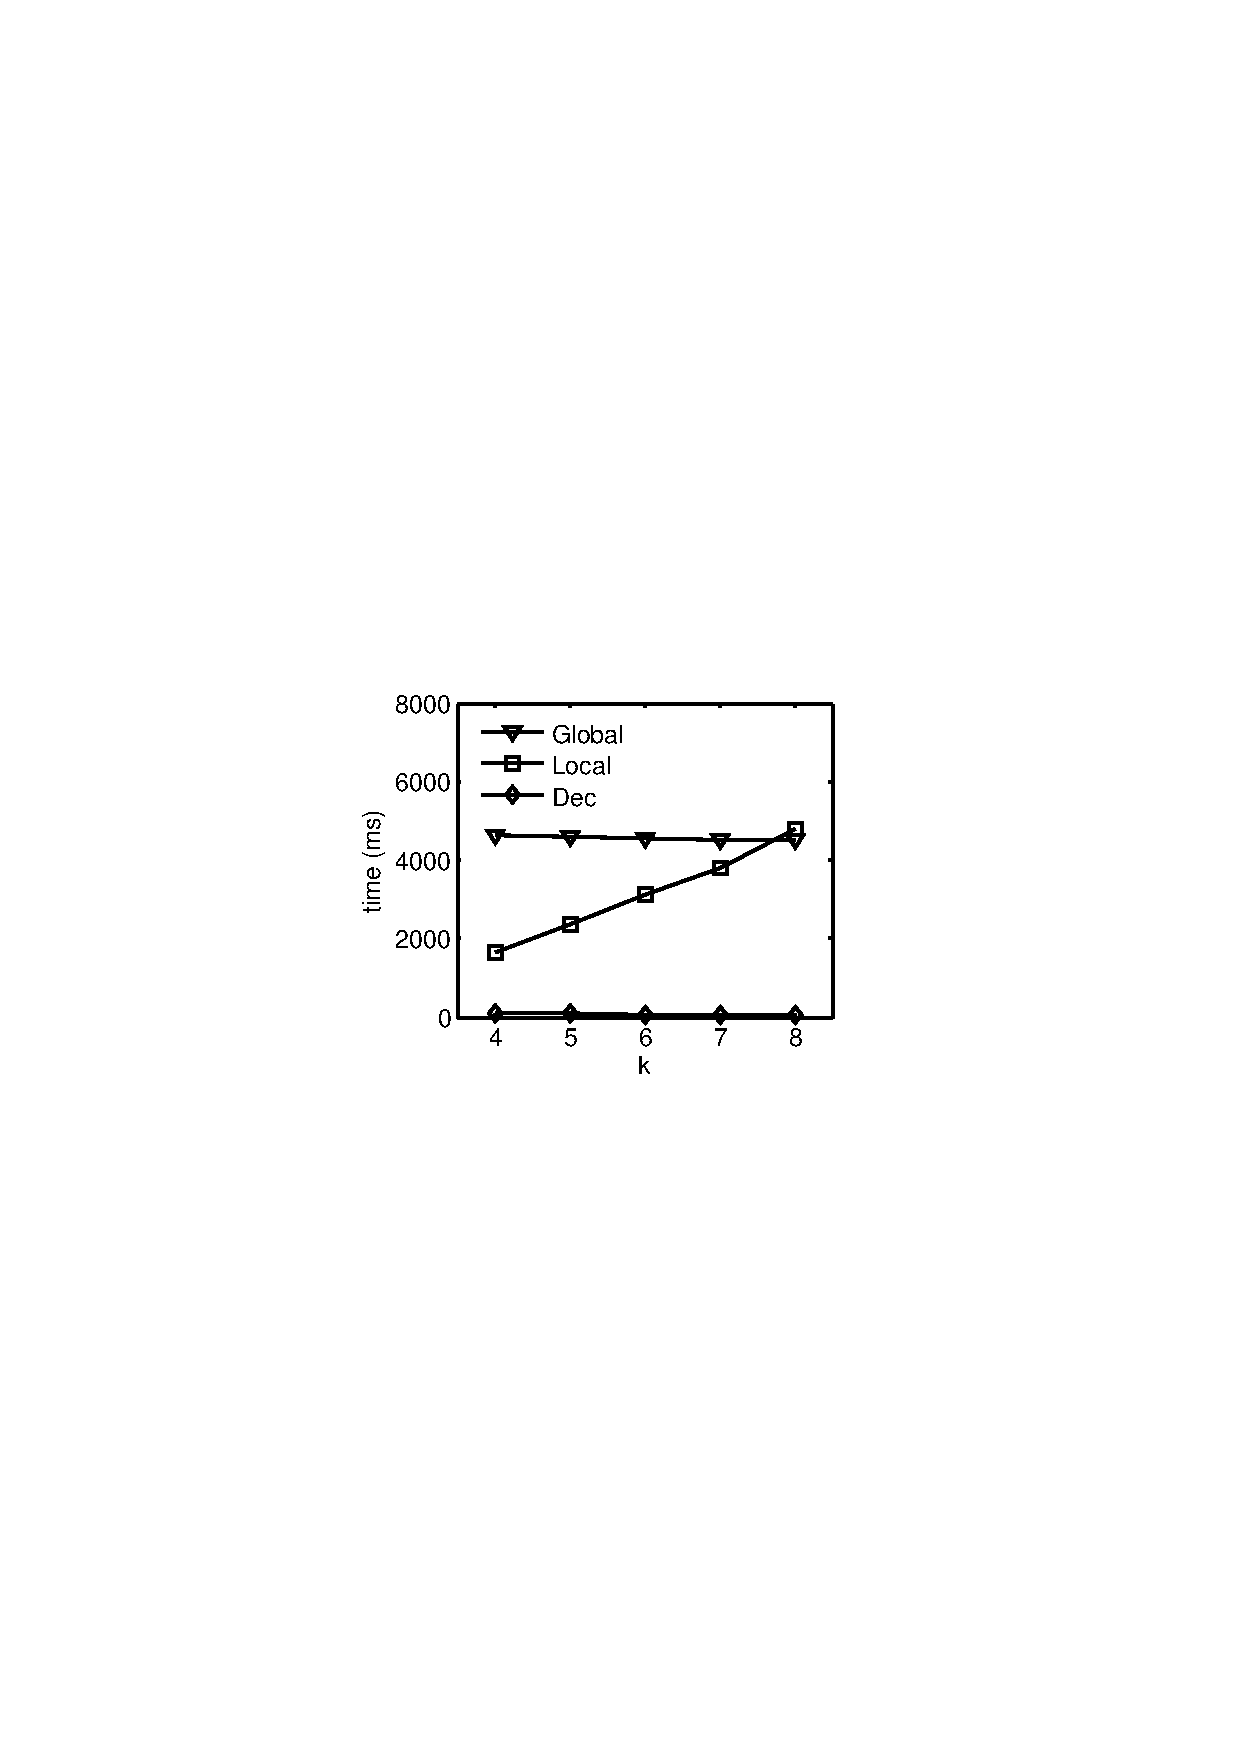
\includegraphics[width=3.725cm]{figures/tencent-comp}
  \end{minipage}
  &
  \begin{minipage}{3.725cm}
	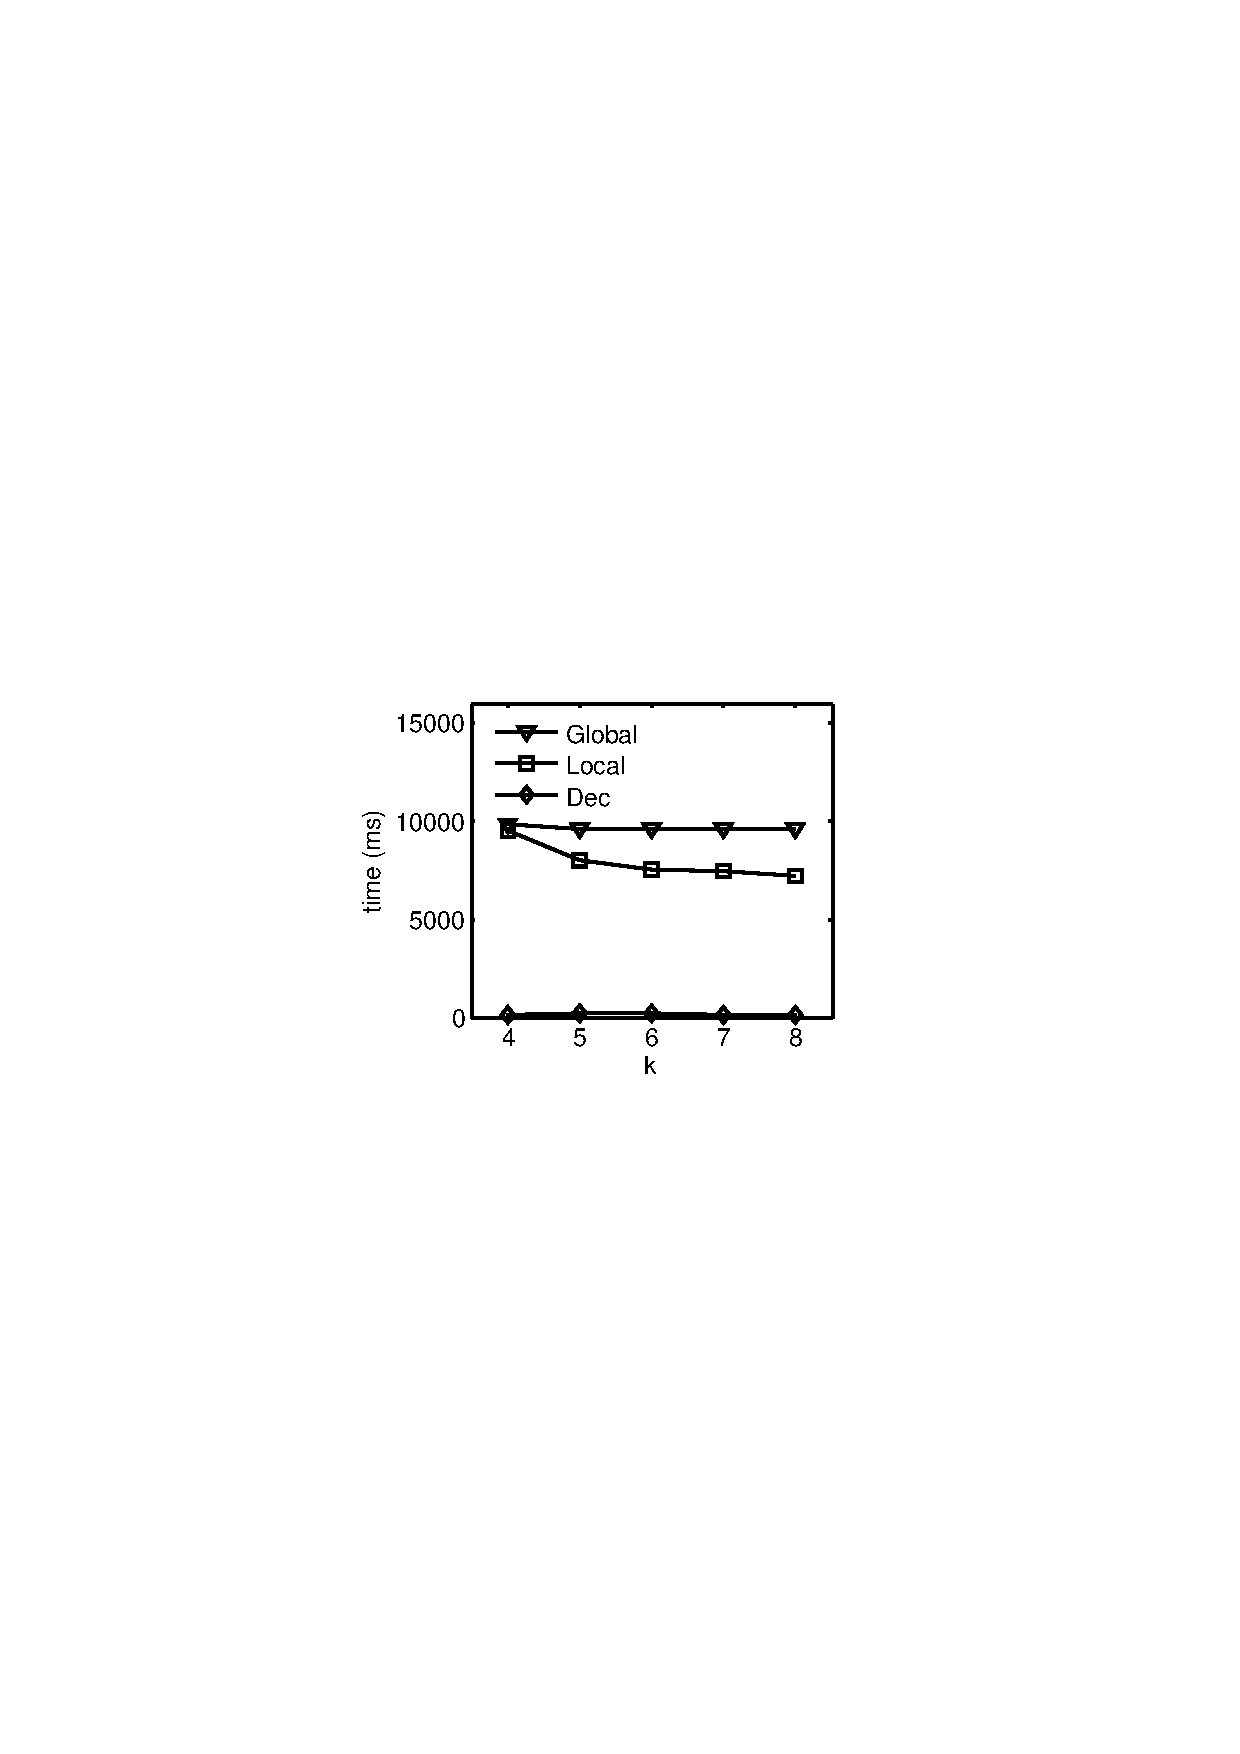
\includegraphics[width=3.725cm]{figures/dbpedia-comp}
  \end{minipage}
  \\
  \small (a) Flickr (efficiency)
  &
  \small (b) DBLP (efficiency)
  &
  \small (c) Tencent (efficiency)
  &
  \small (d) DBpedia (efficiency)
  \\

  \begin{minipage}{3.725cm}
	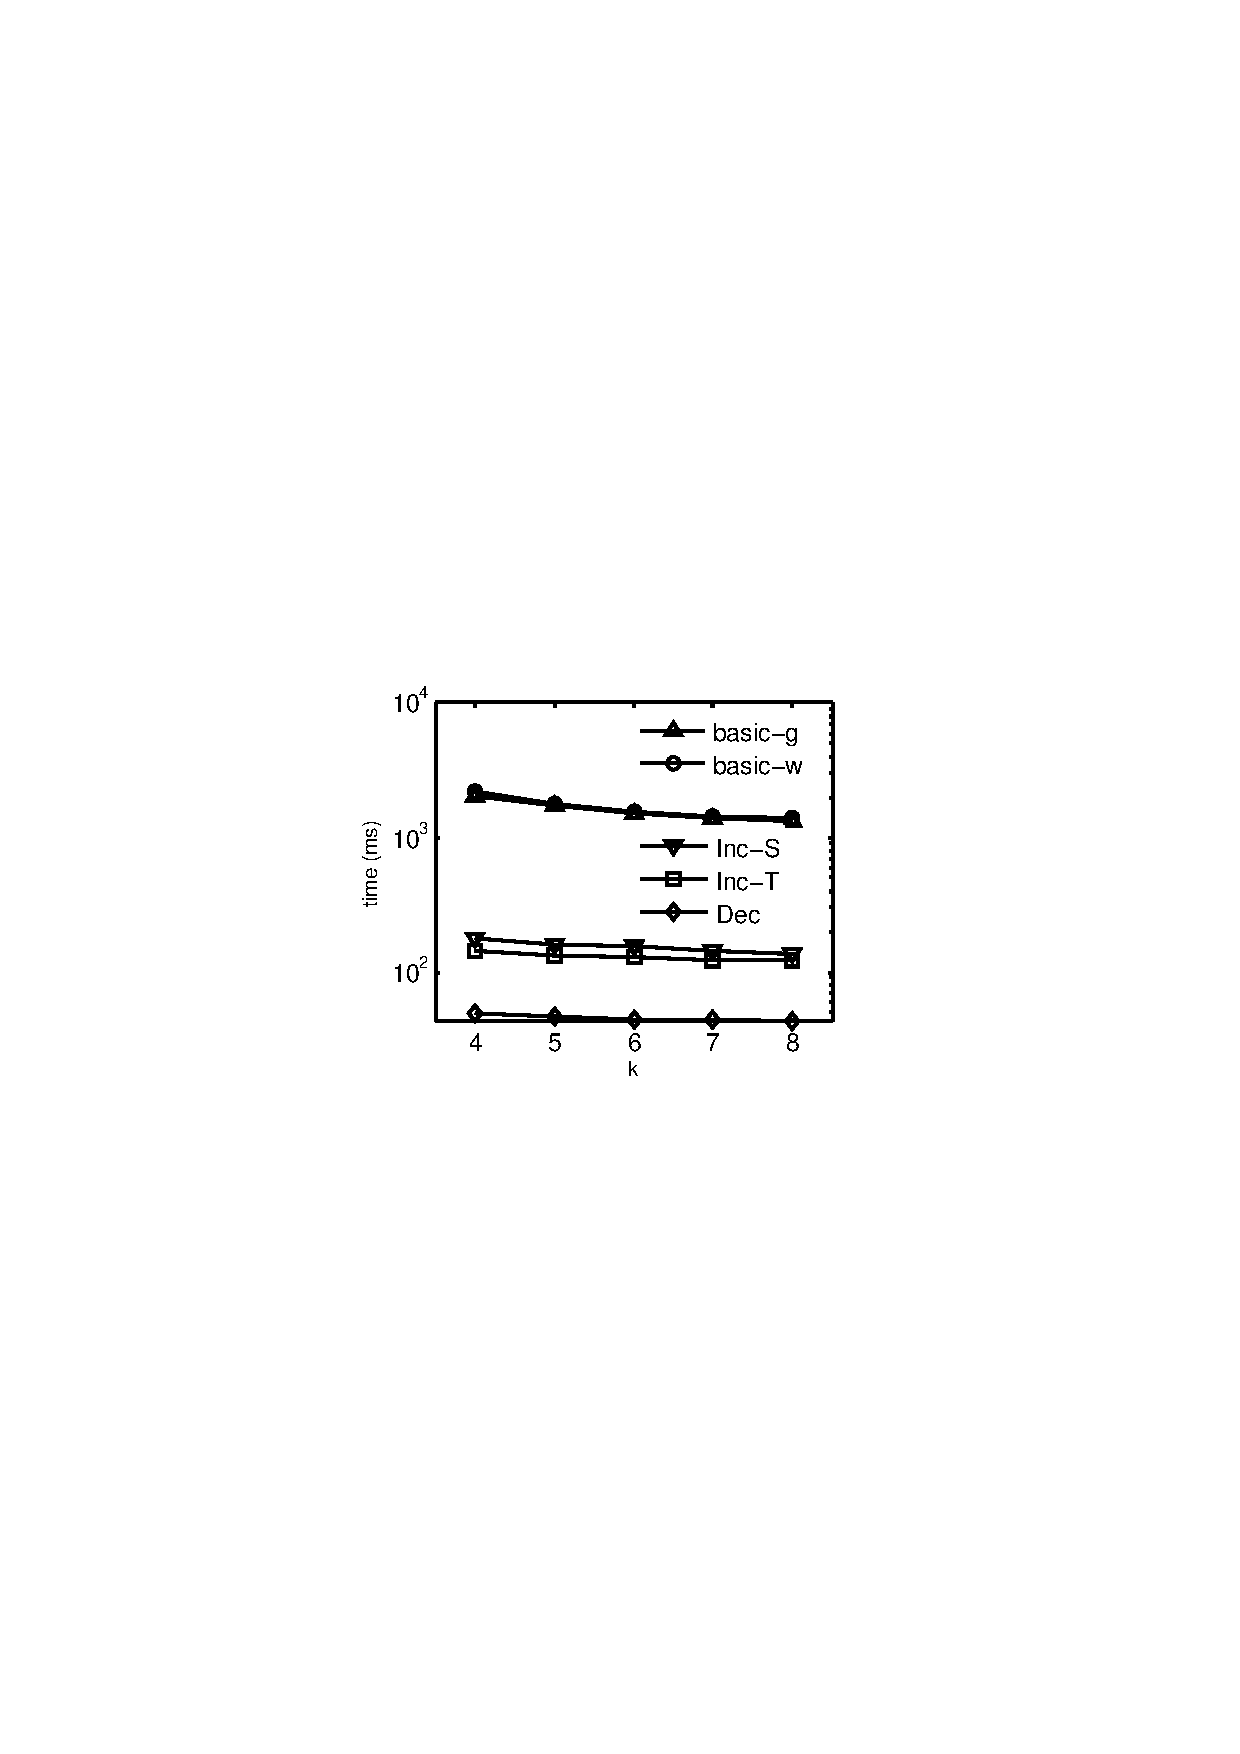
\includegraphics[width=3.725cm]{figures/flickr-k}
  \end{minipage}
  &
  \begin{minipage}{3.725cm}
	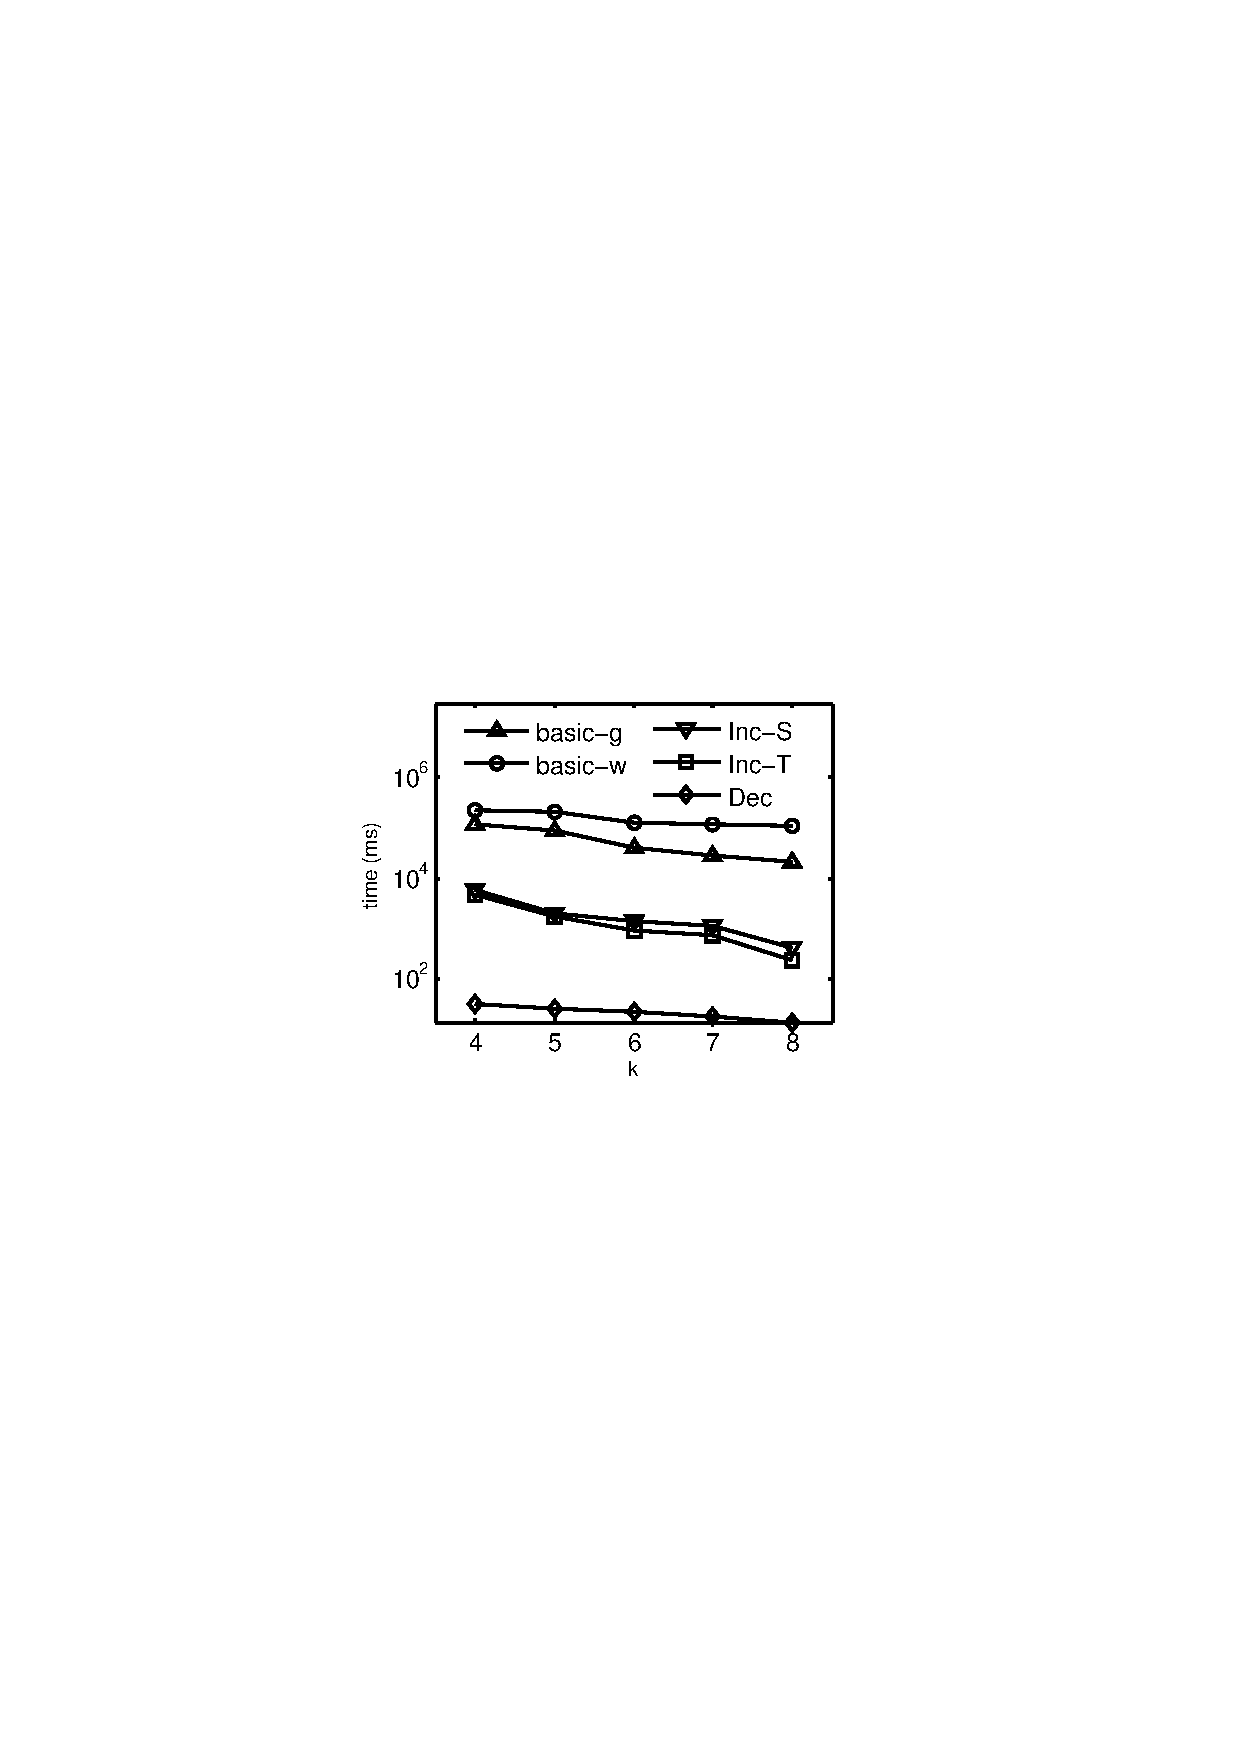
\includegraphics[width=3.725cm]{figures/dblp-k}
  \end{minipage}
  &
  \begin{minipage}{3.725cm}
	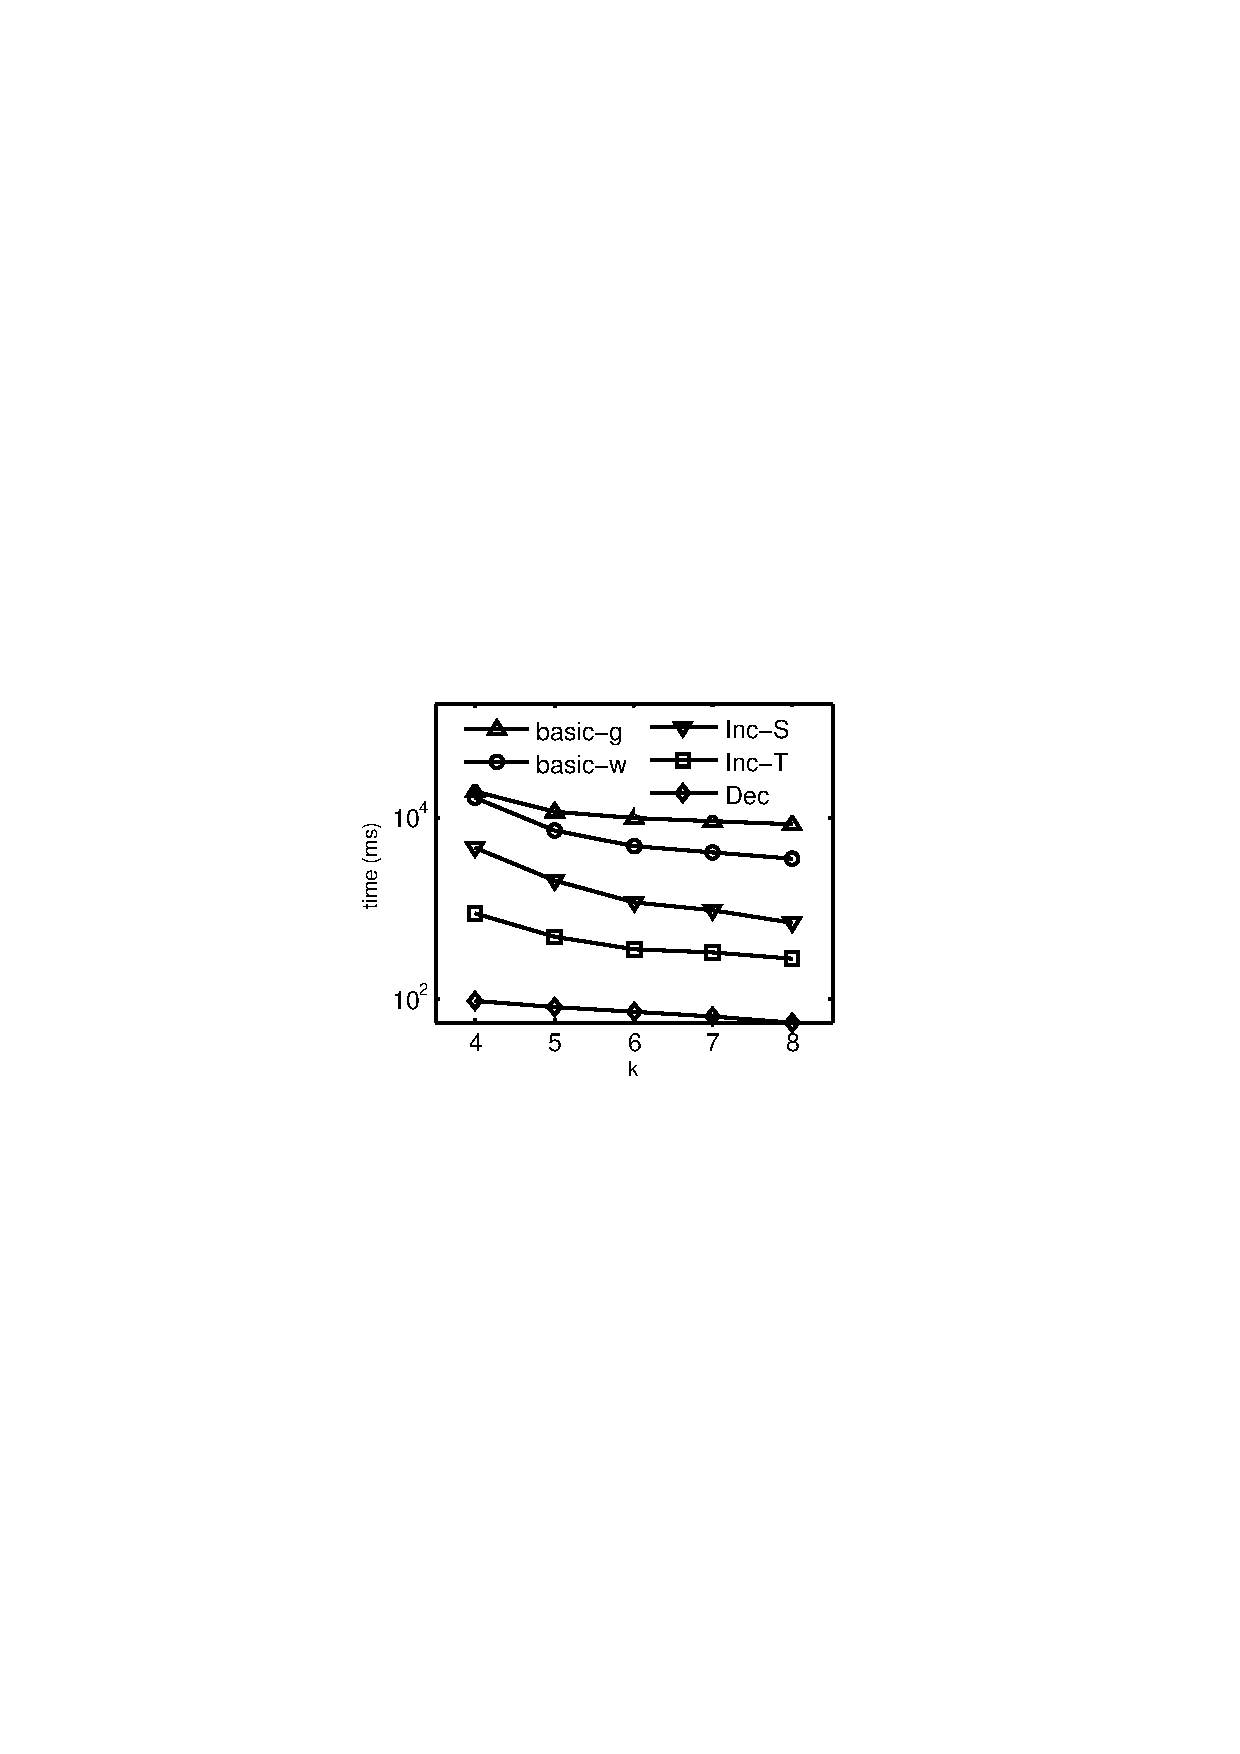
\includegraphics[width=3.725cm]{figures/tencent-k}
  \end{minipage}
  &
  \begin{minipage}{3.725cm}
	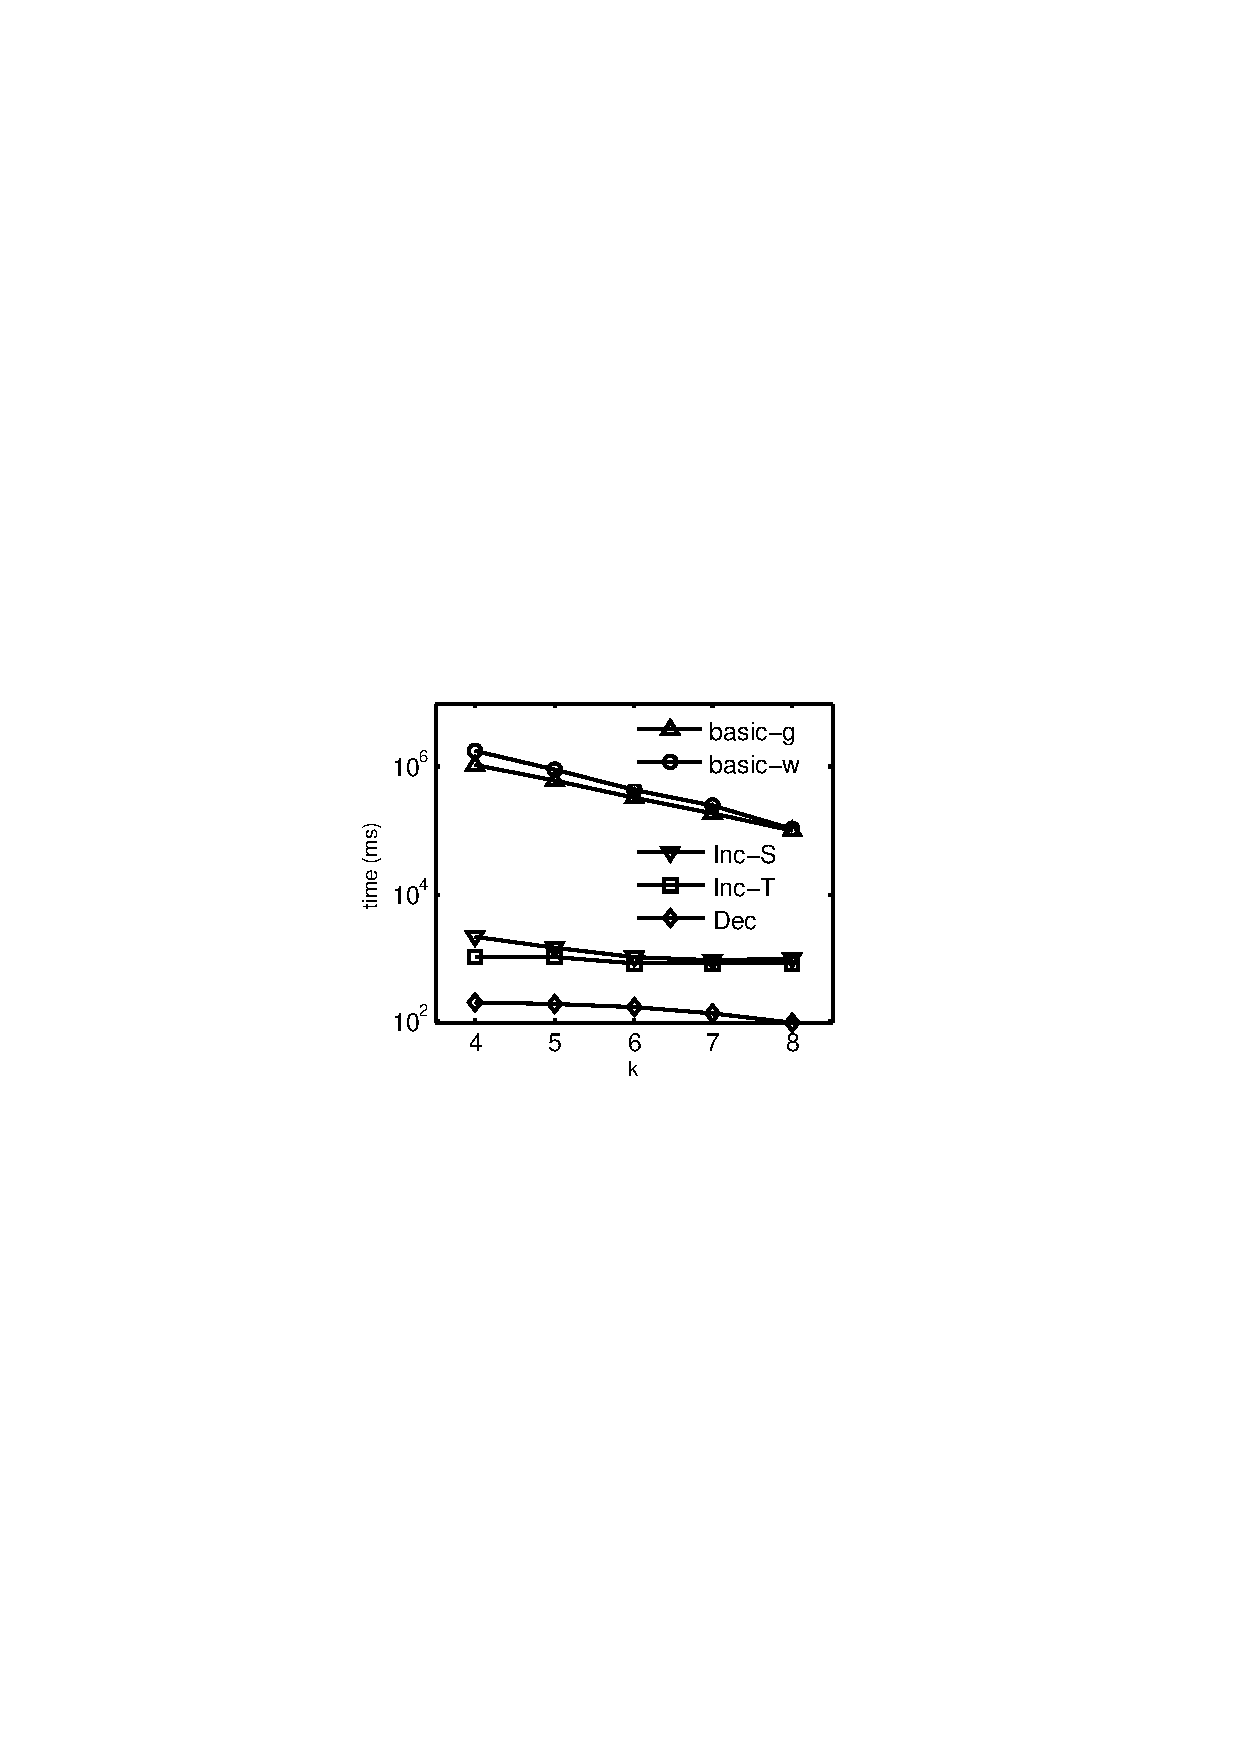
\includegraphics[width=3.725cm]{figures/dbpedia-k}
  \end{minipage}
  \\
  \small (e) Flickr (effect of $k$)
  &
  \small (f) DBLP (effect of $k$)
  &
  \small (g) Tencent (effect of $k$)
  &
  \small (h) DBpedia (effect of $k$)
  \\

  \begin{minipage}{3.725cm}
	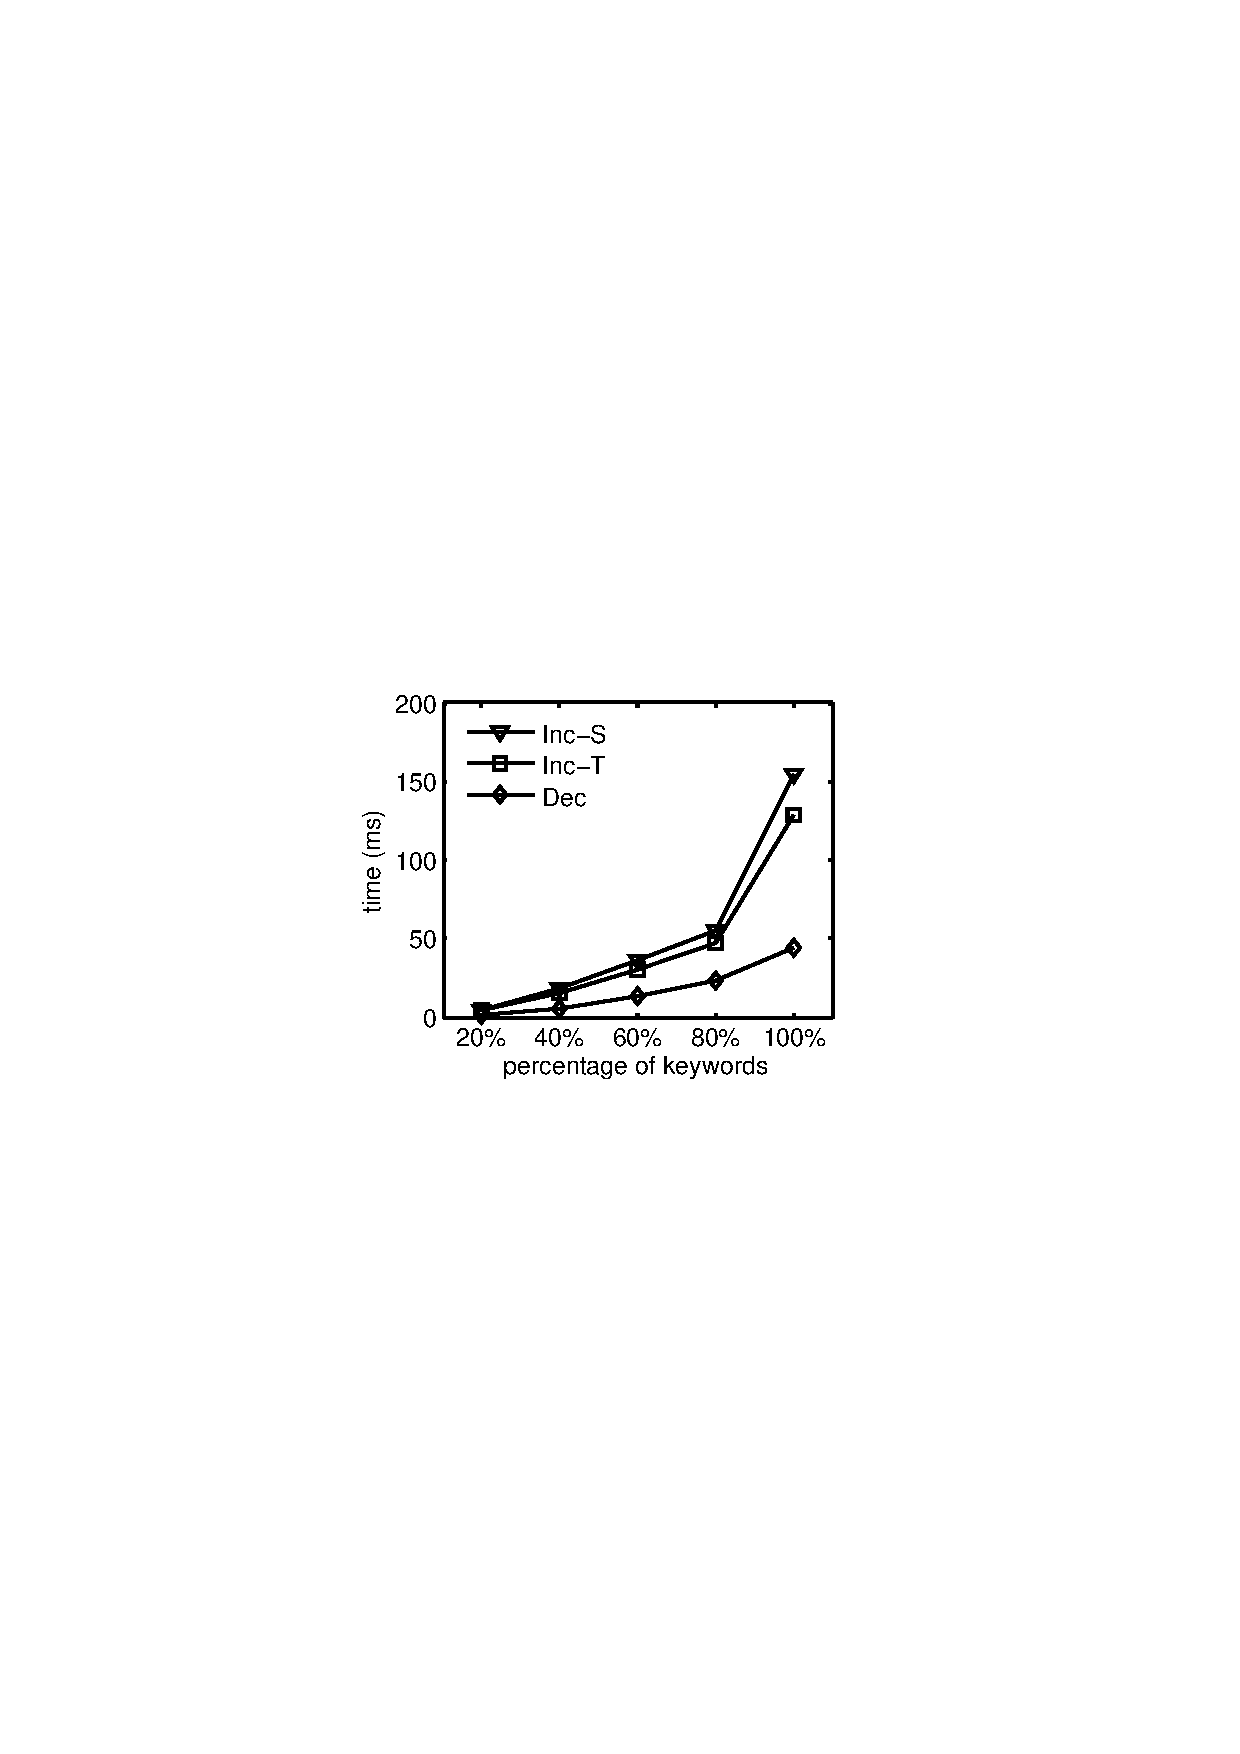
\includegraphics[width=3.725cm]{figures/flickr-keyword}
  \end{minipage}
  &
  \begin{minipage}{3.725cm}
	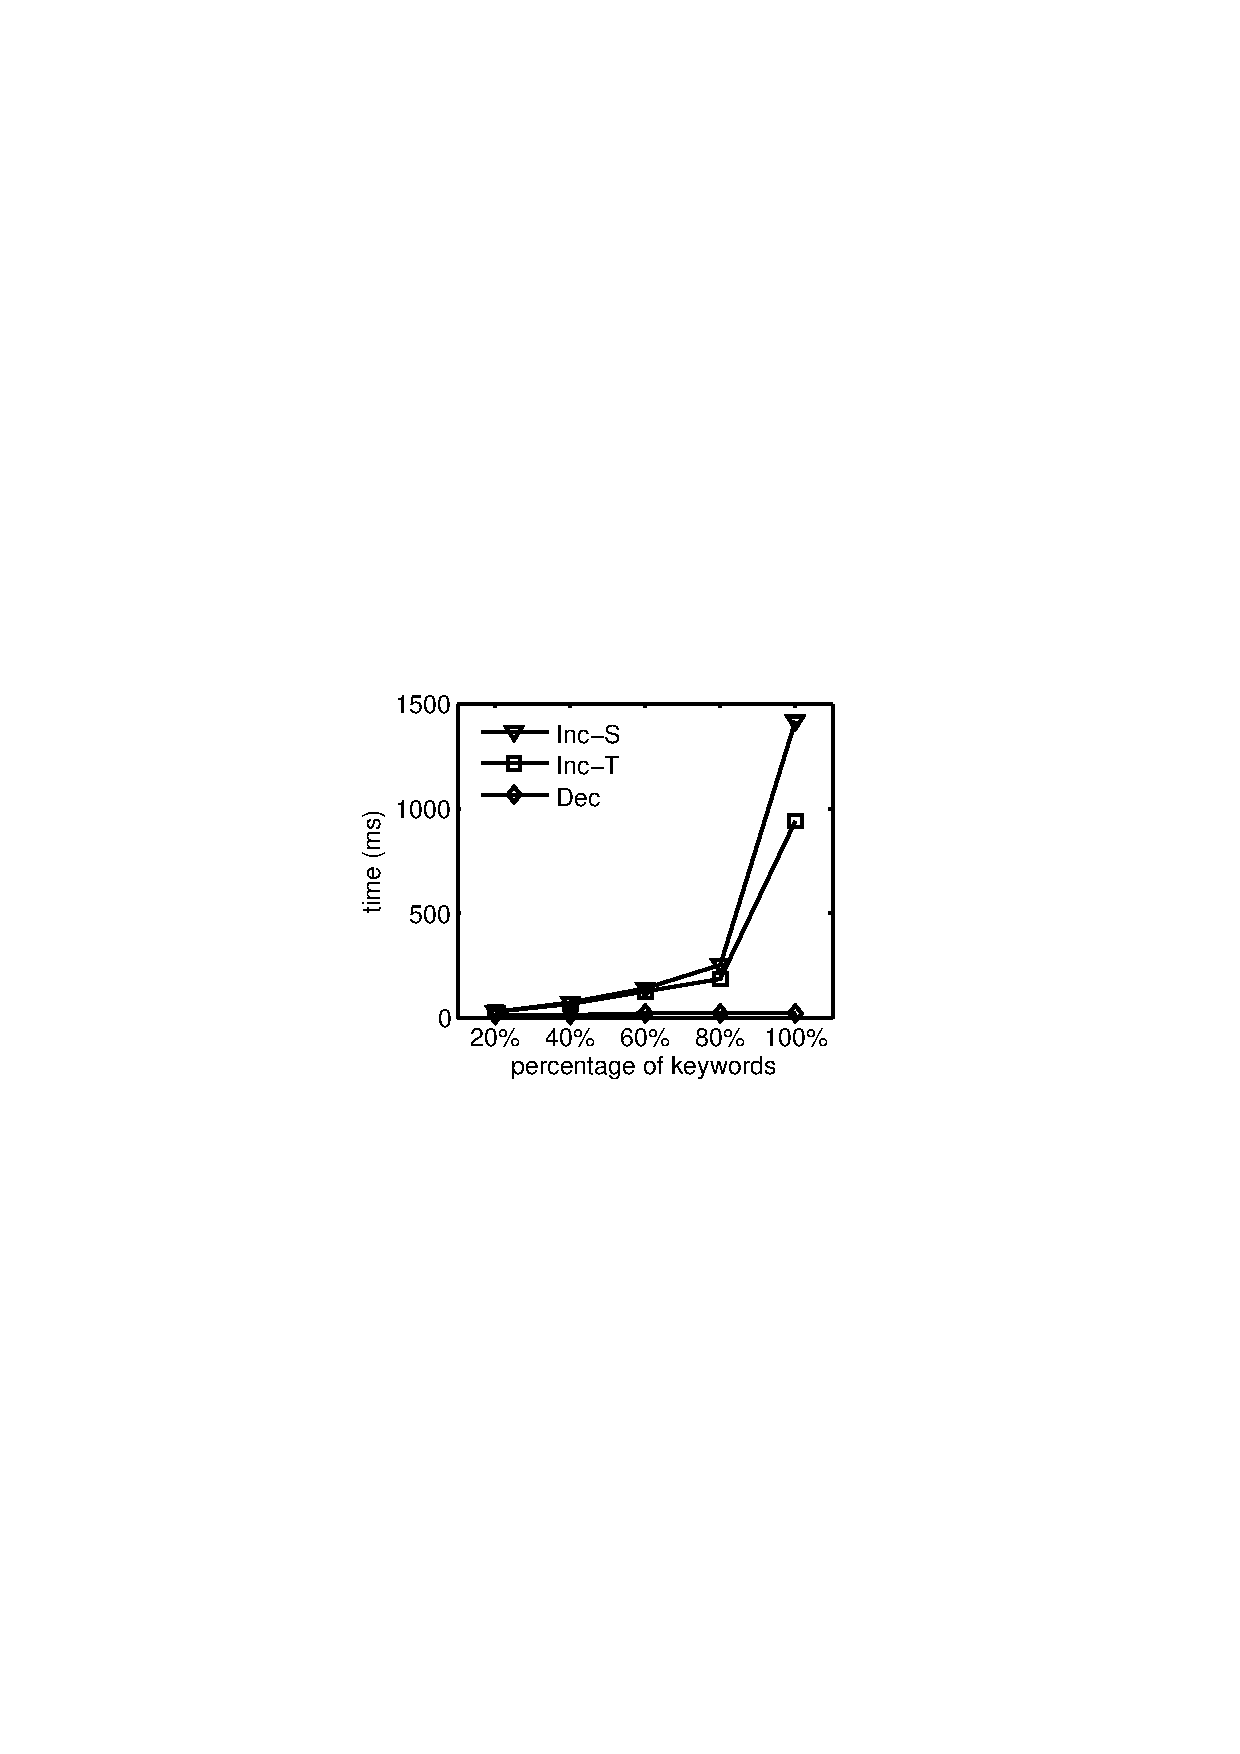
\includegraphics[width=3.725cm]{figures/dblp-keyword}
  \end{minipage}
  &
  \begin{minipage}{3.725cm}
	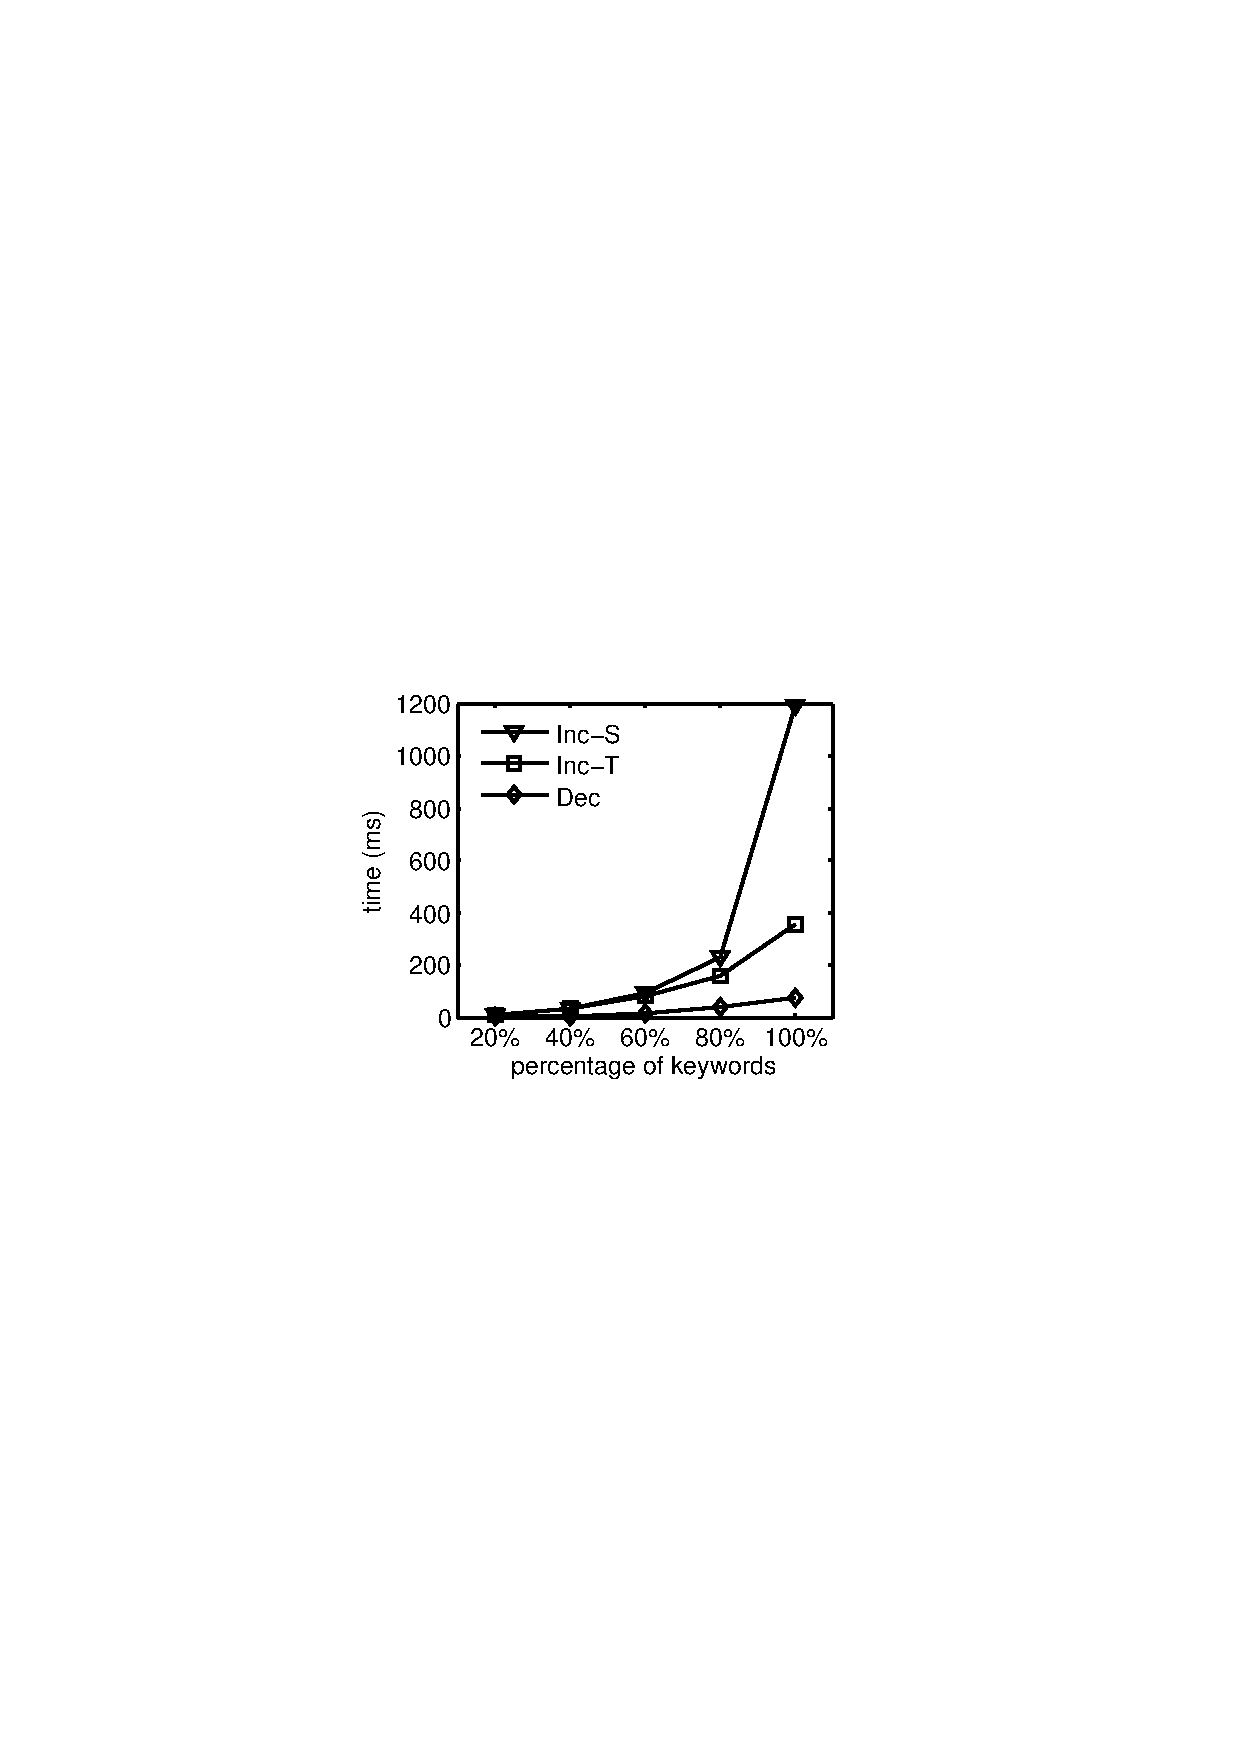
\includegraphics[width=3.725cm]{figures/tencent-keyword}
  \end{minipage}
  &
  \begin{minipage}{3.725cm}
	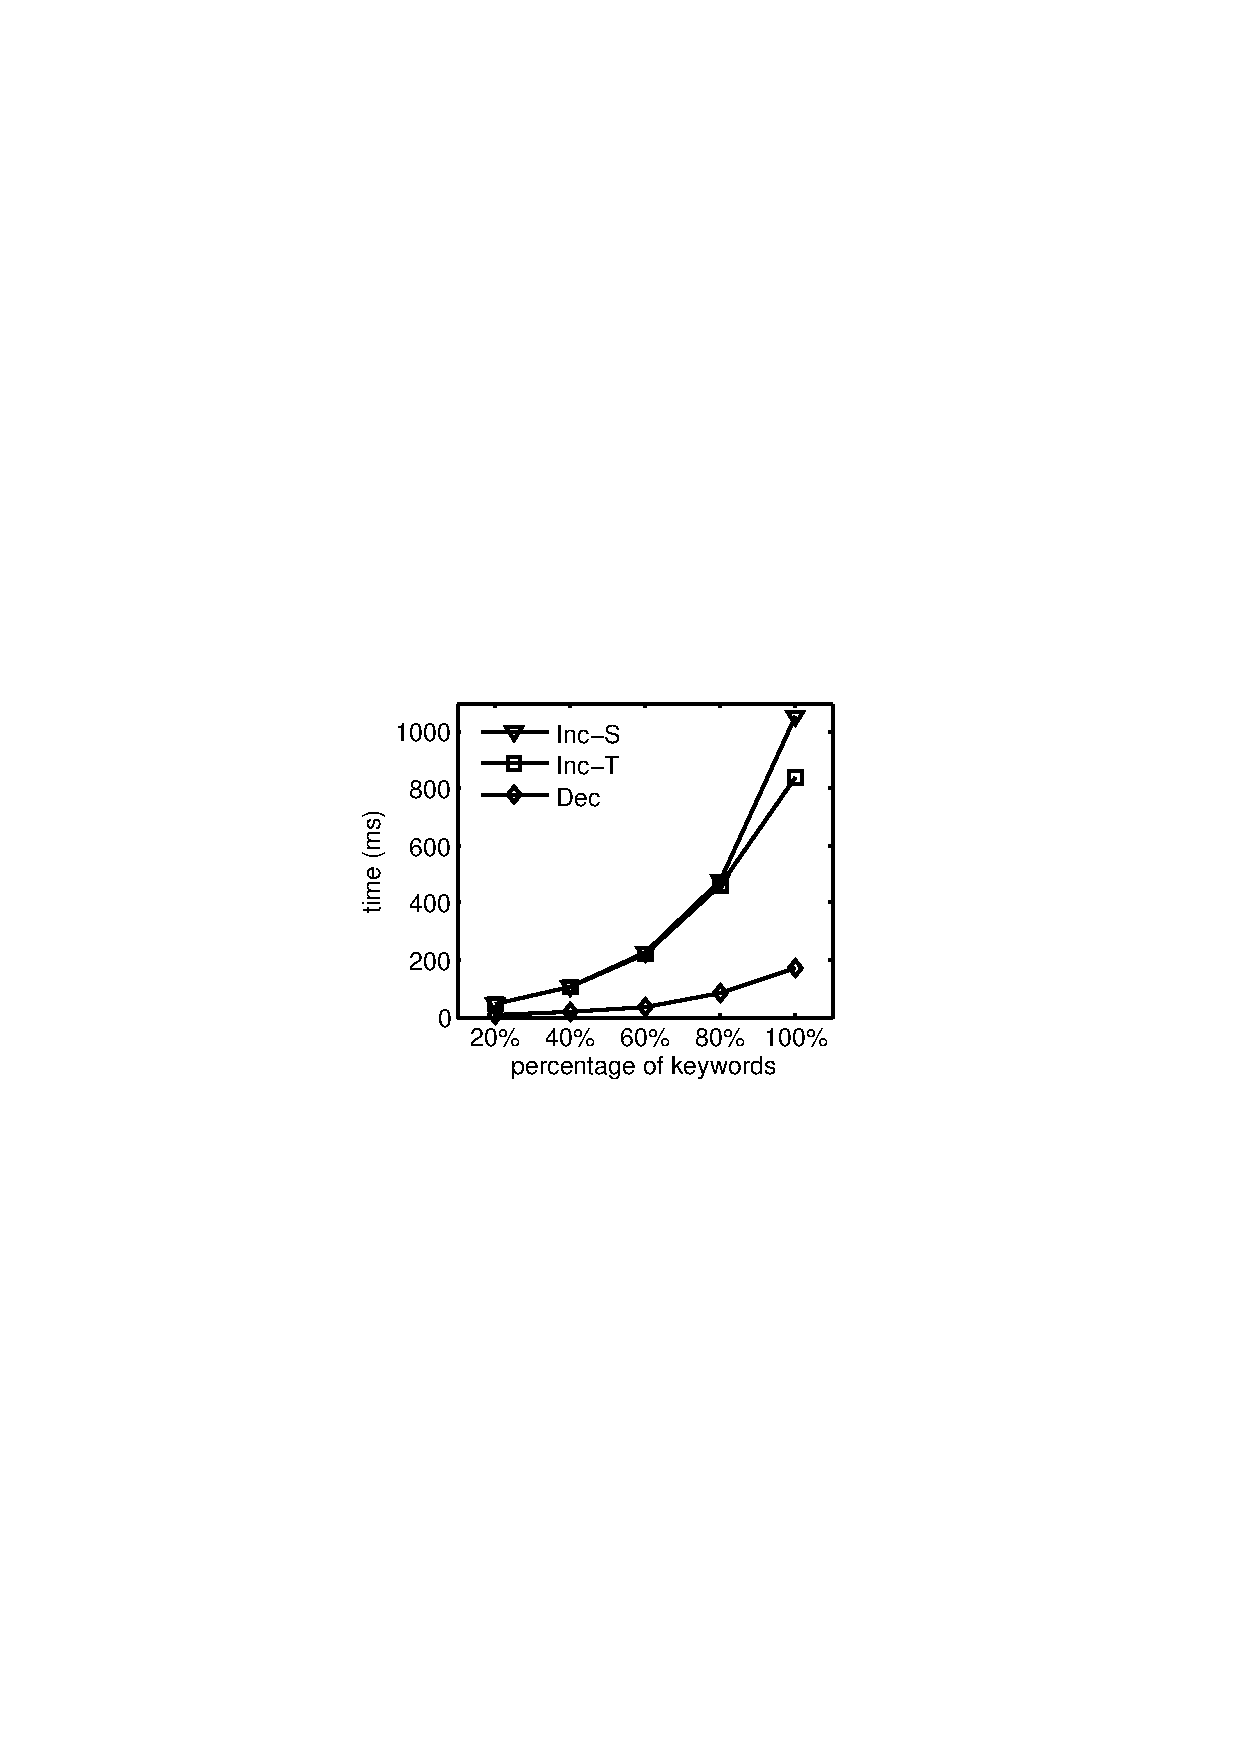
\includegraphics[width=3.725cm]{figures/dbpedia-keyword}
  \end{minipage}
  \\
  \small (i) Flickr (keyword scalab.)
  &
  \small (j) DBLP (keyword scalab.)
  &
  \small (k) Tencent (keyword scalab.)
  &
  \small (l) DBpedia (keyword scalab.)
  \\

  \begin{minipage}{3.725cm}
	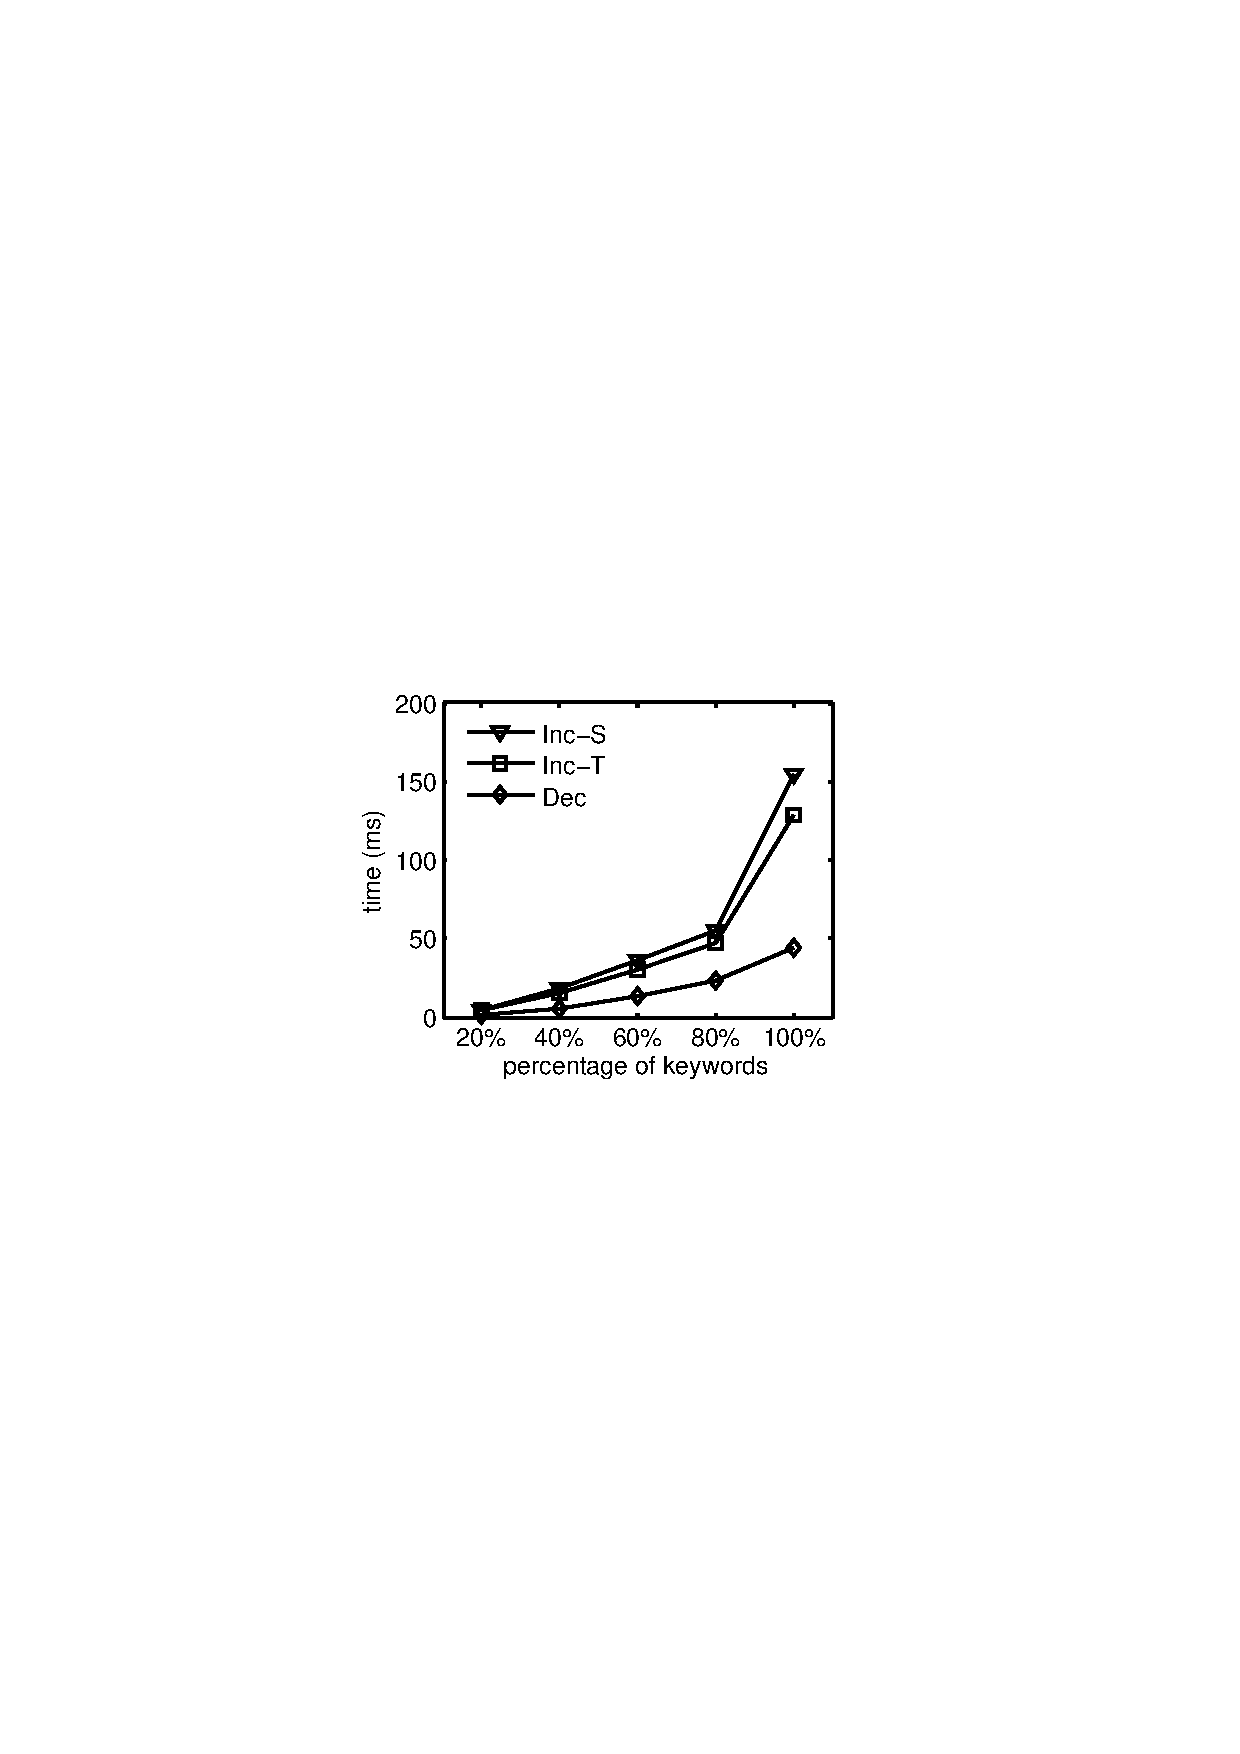
\includegraphics[width=3.725cm]{figures/flickr-keyword}
  \end{minipage}
  &
  \begin{minipage}{3.725cm}
	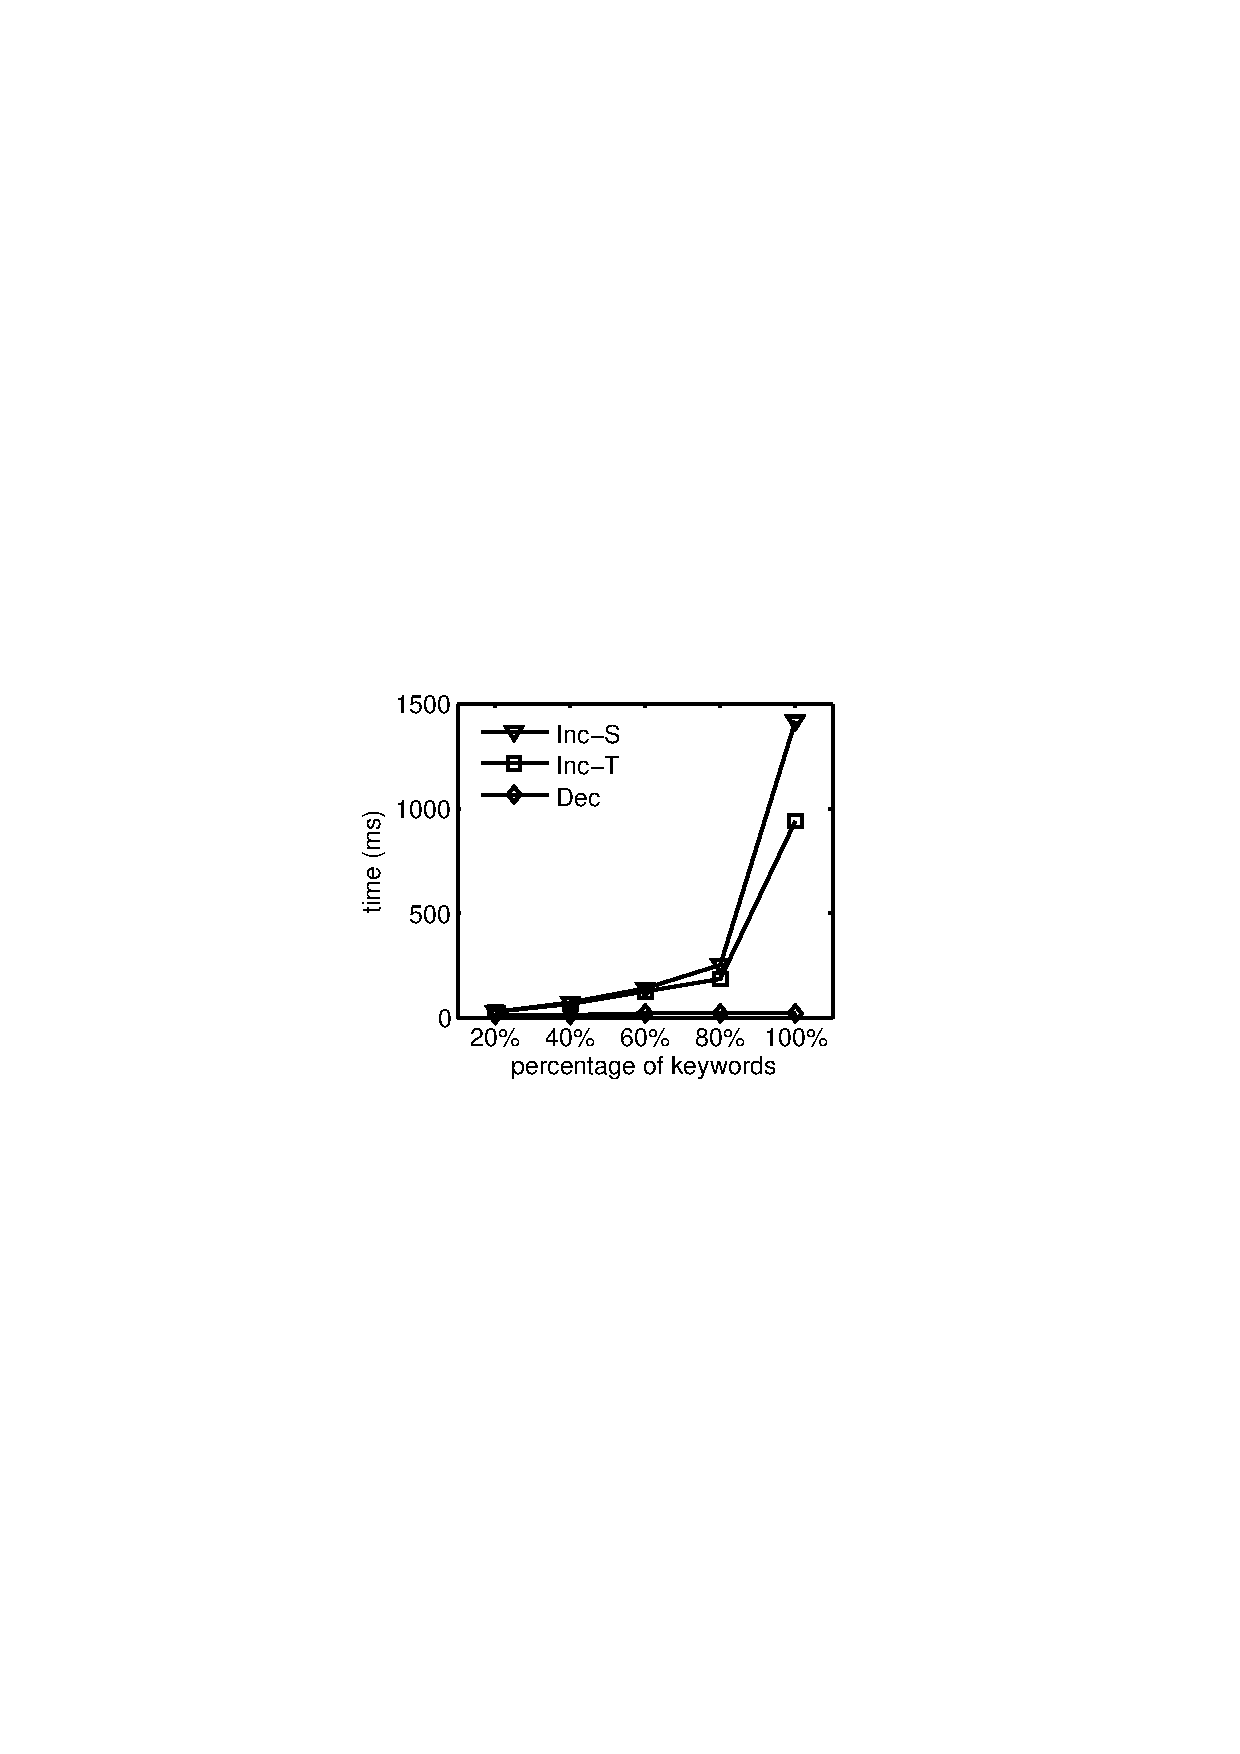
\includegraphics[width=3.725cm]{figures/dblp-keyword}
  \end{minipage}
  &
  \begin{minipage}{3.725cm}
	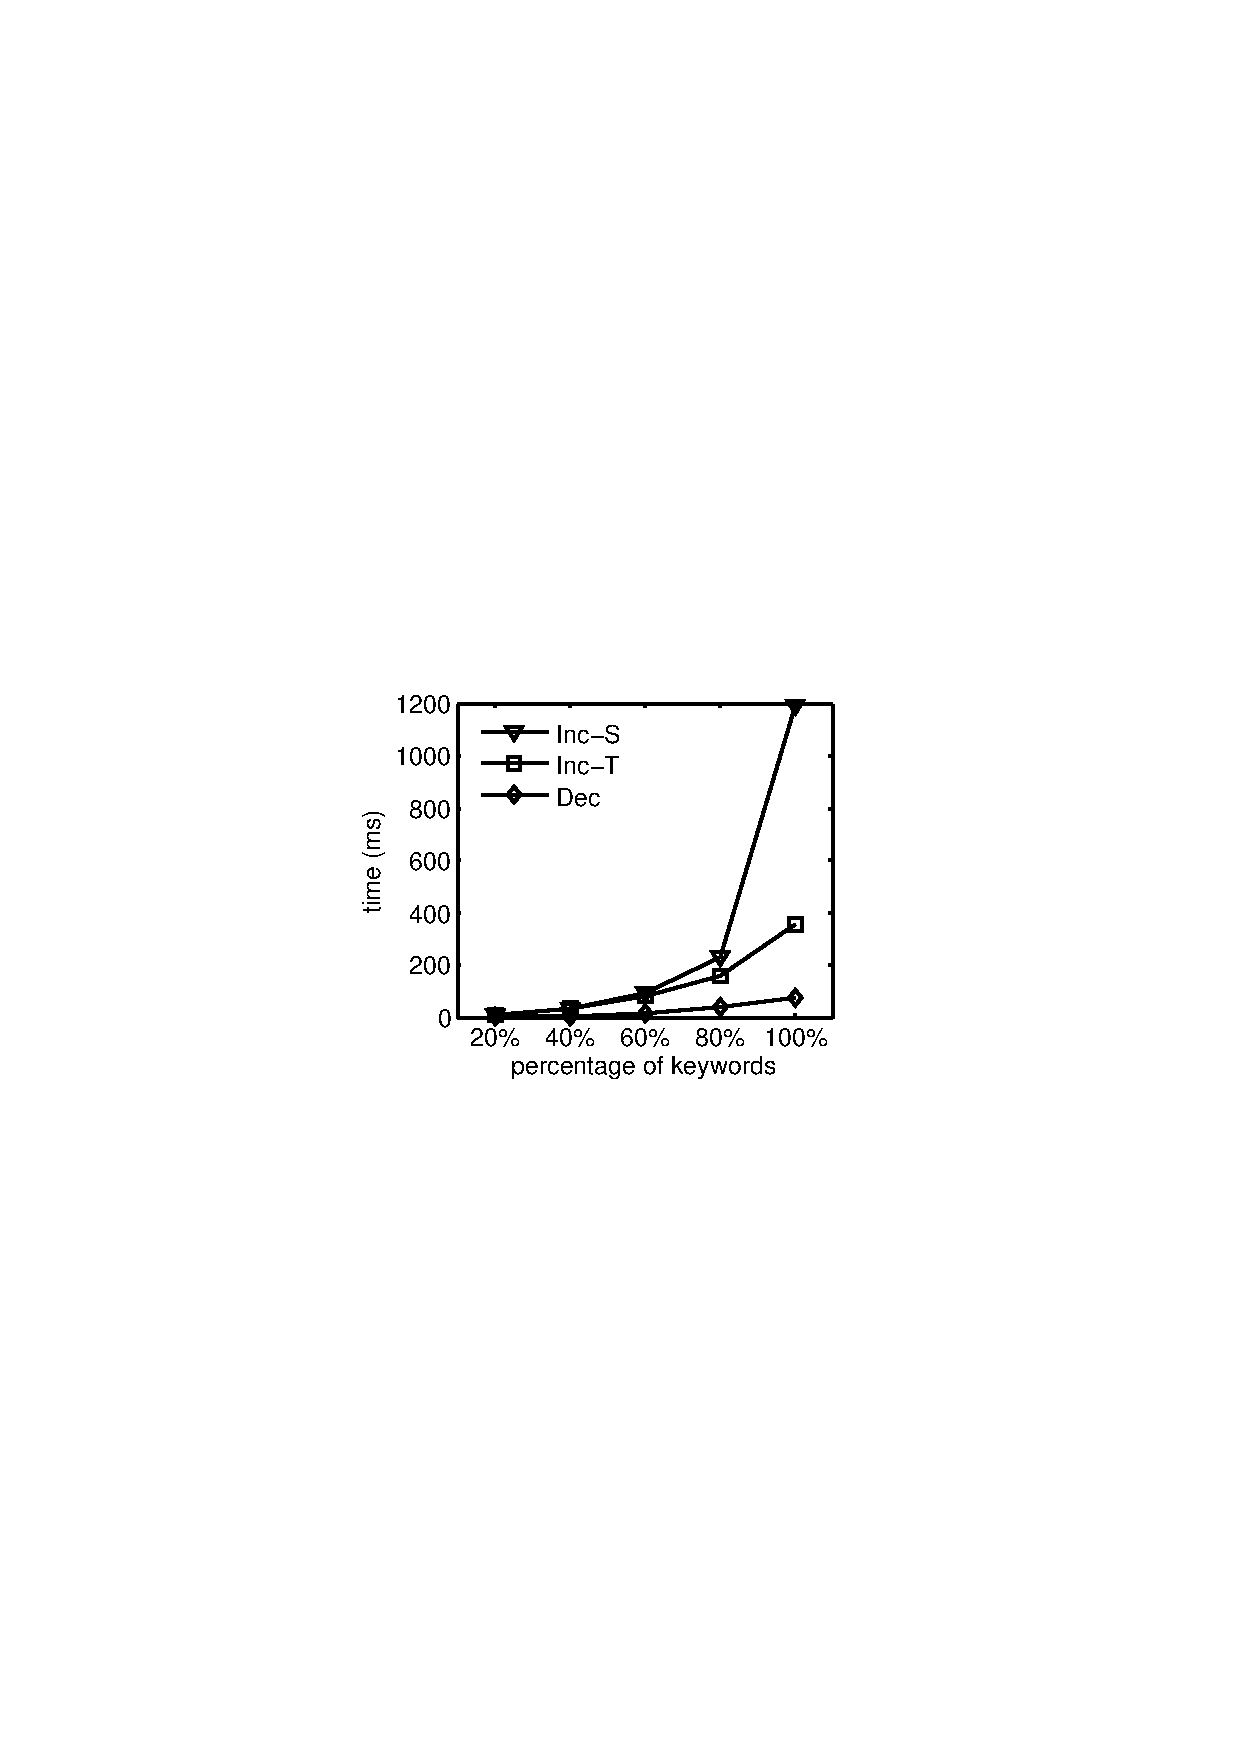
\includegraphics[width=3.725cm]{figures/tencent-keyword}
  \end{minipage}
  &
  \begin{minipage}{3.725cm}
	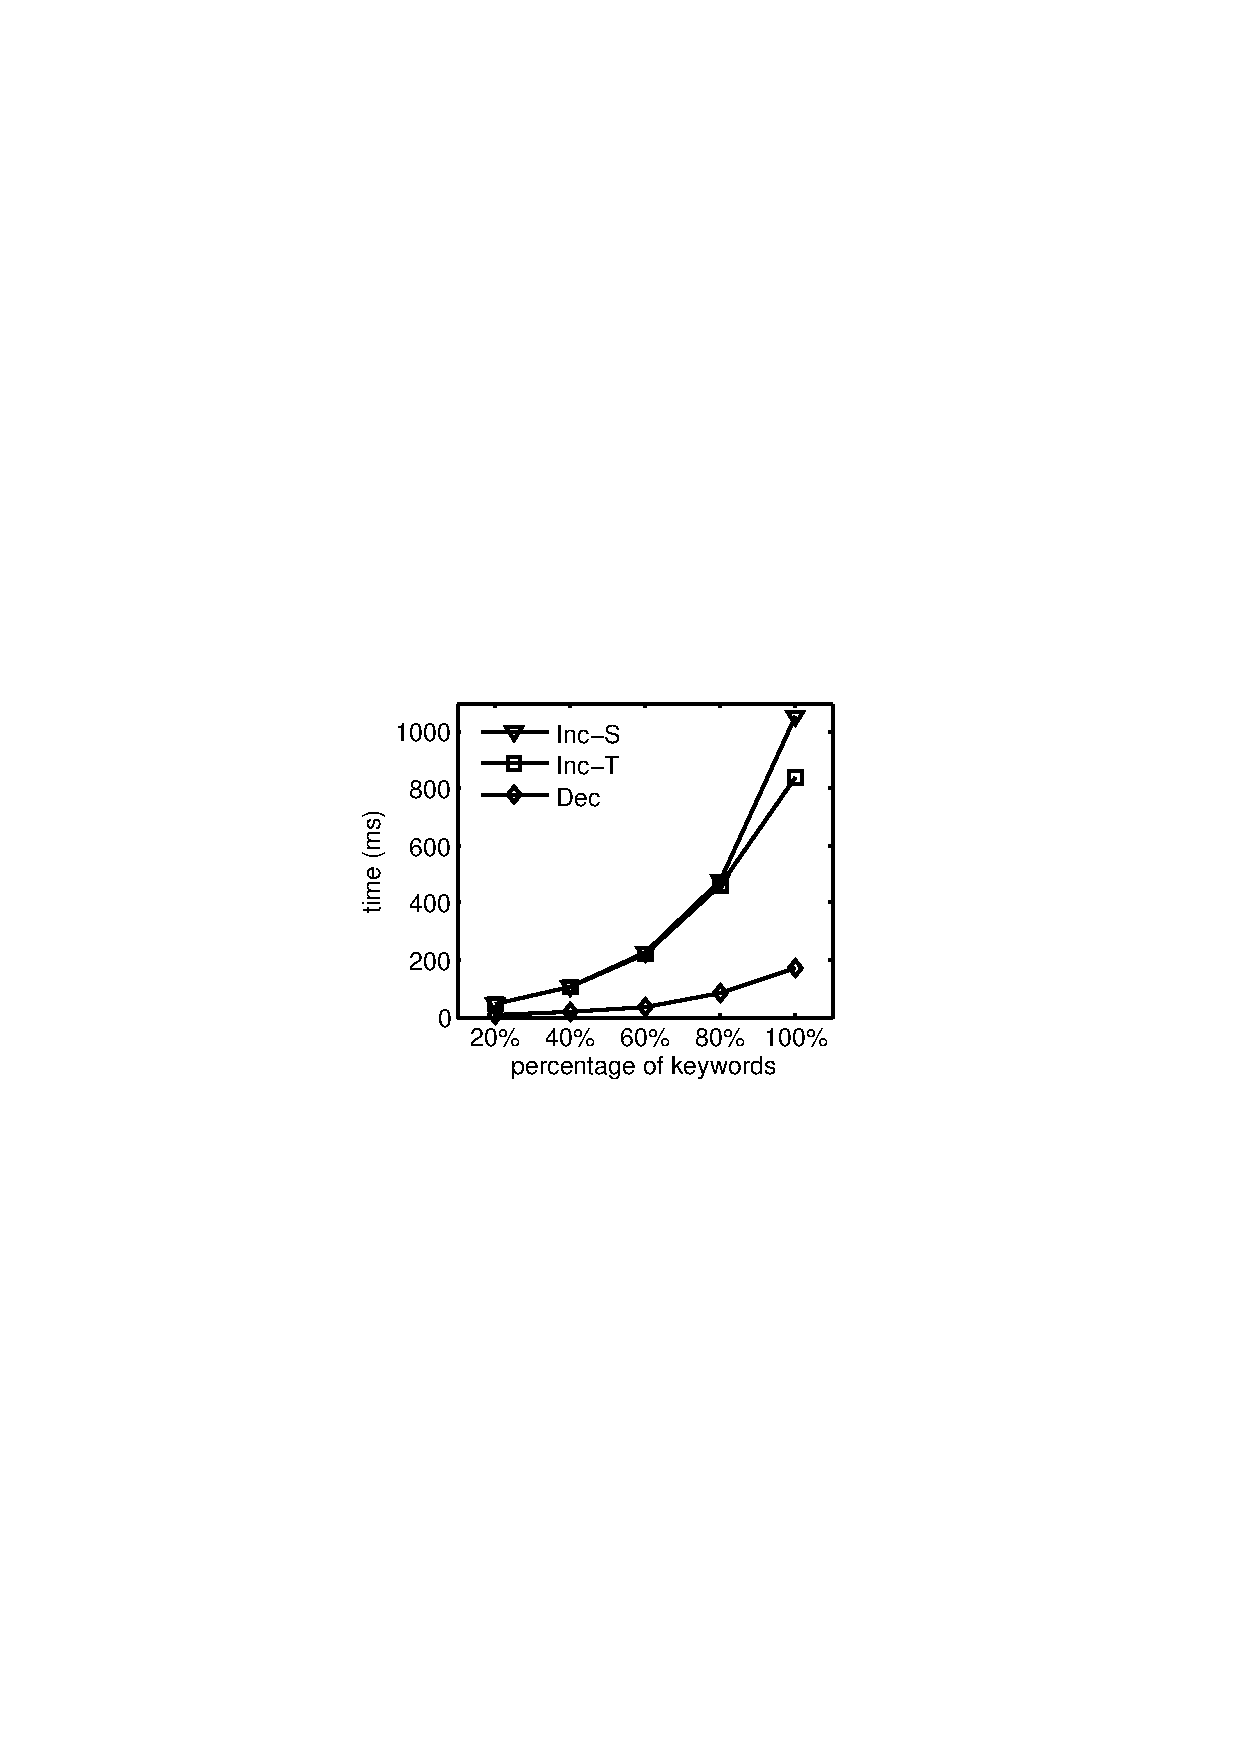
\includegraphics[width=3.725cm]{figures/dbpedia-keyword}
  \end{minipage}
  \\
  \small (m) Flickr (vertex scalab.)
  &
  \small (n) DBLP (vertex scalab.)
  &
  \small (o) Tencent (vertex scalab.)
  &
  \small (p) DBpedia (vertex scalab.)
  \\

  \begin{minipage}{3.725cm}
	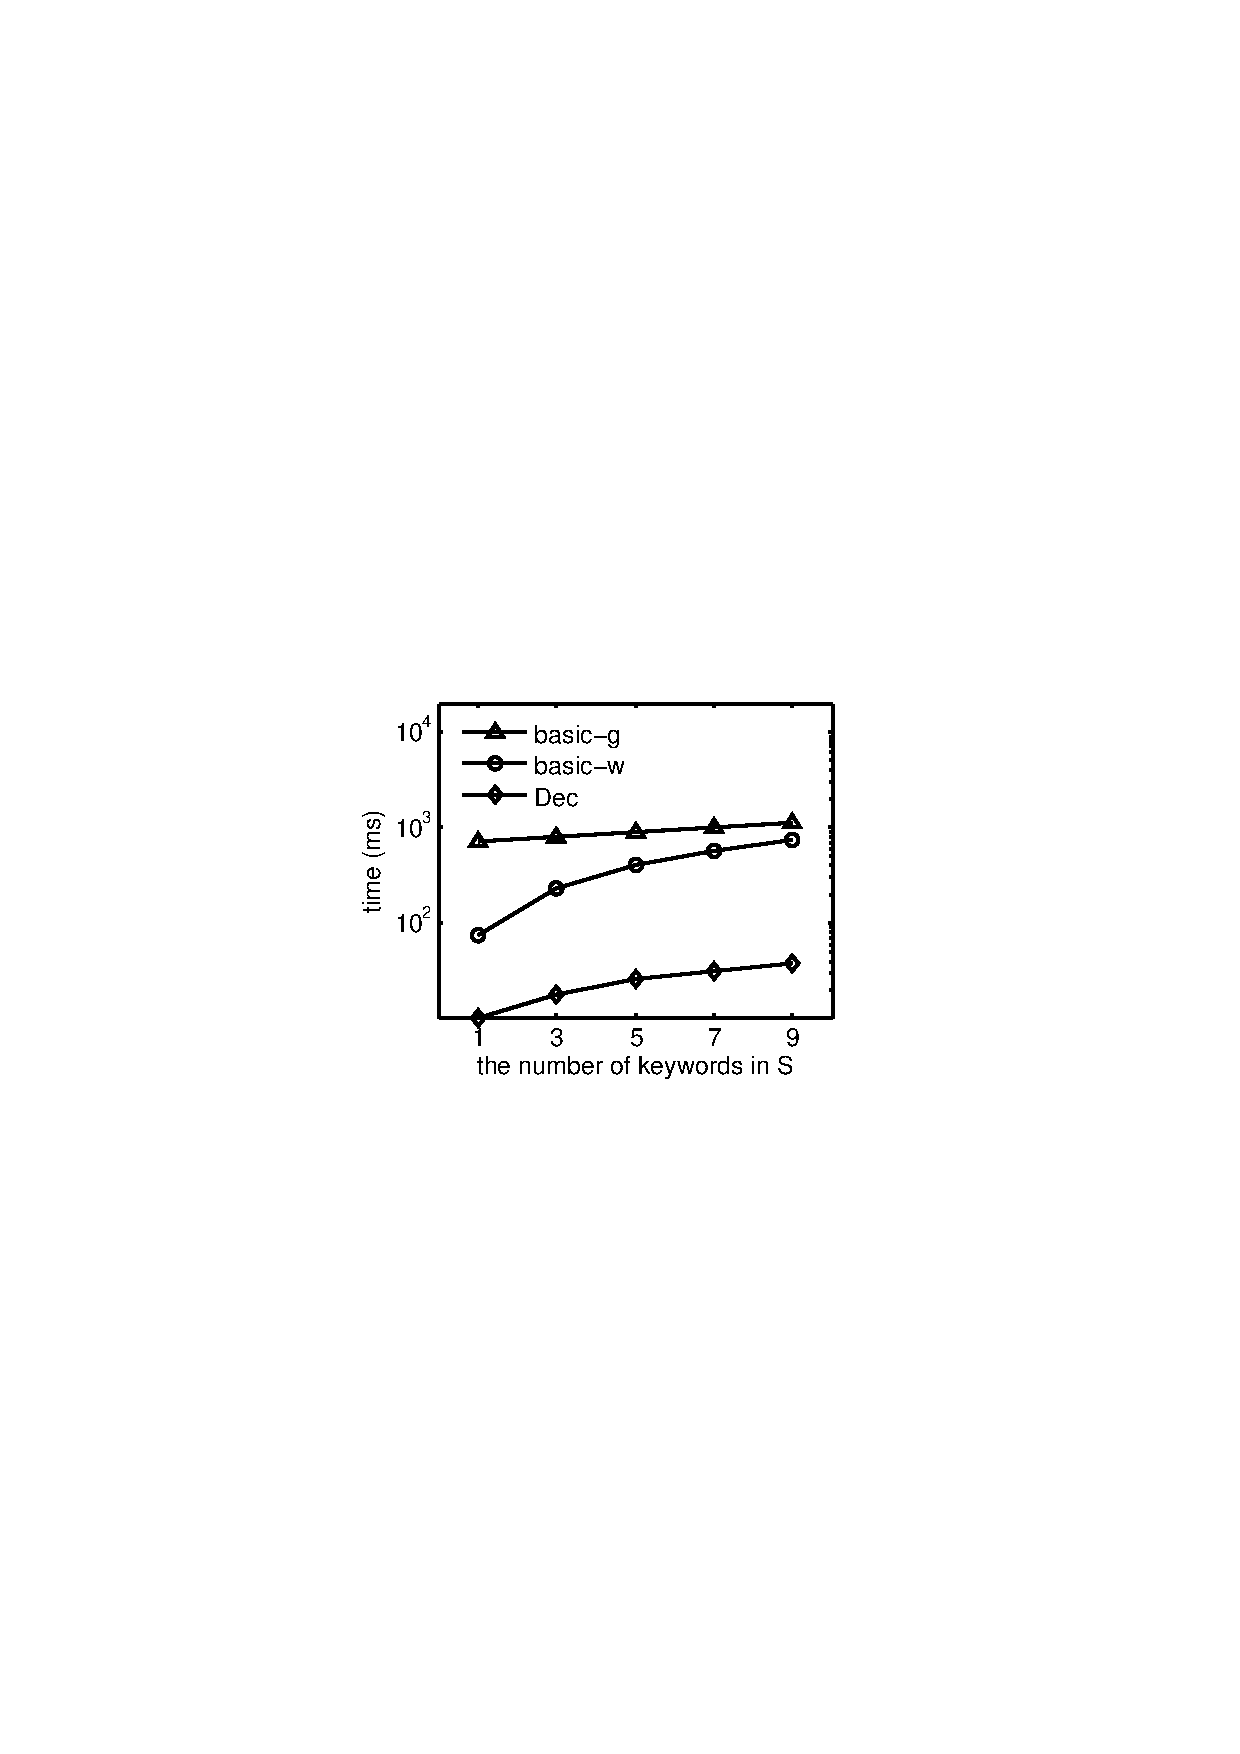
\includegraphics[width=3.725cm]{figures/flickr-s}
  \end{minipage}
  &
  \begin{minipage}{3.725cm}
	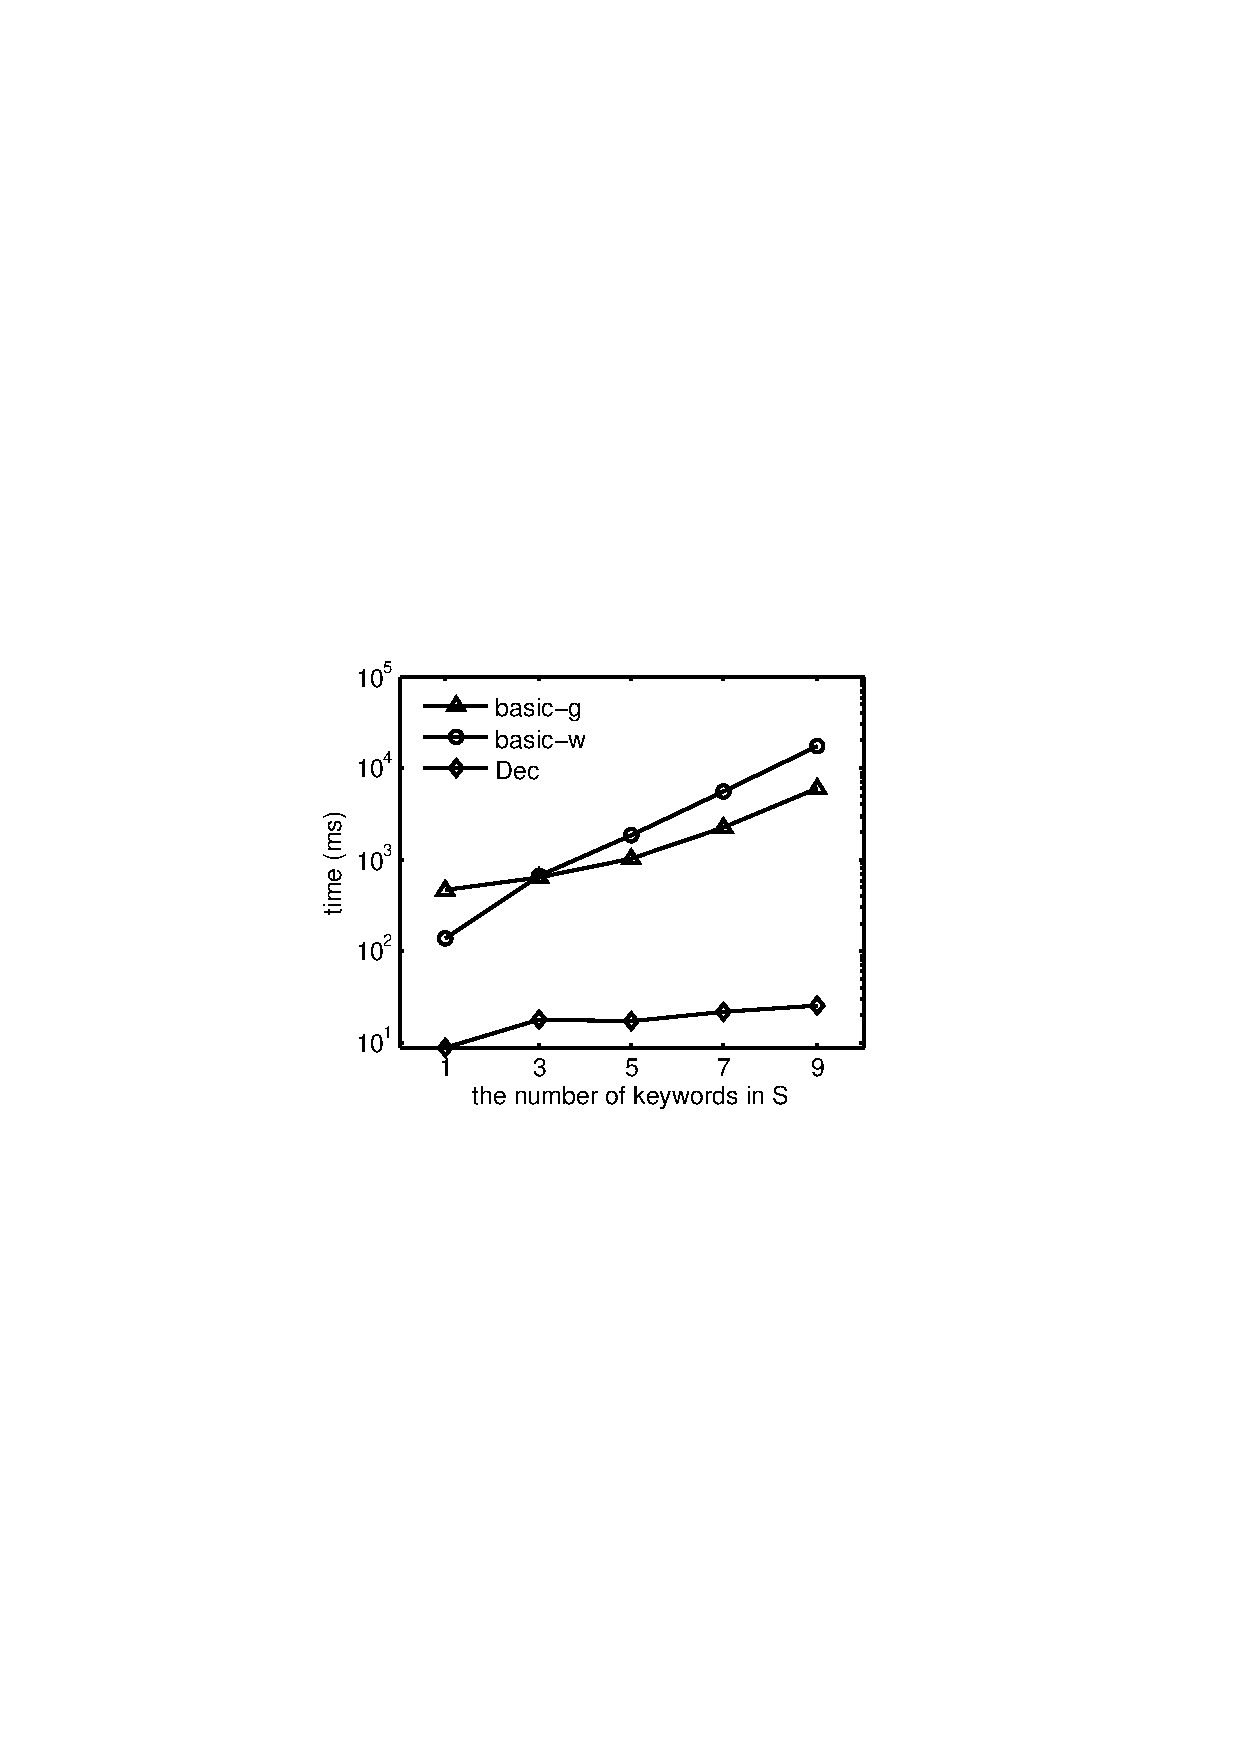
\includegraphics[width=3.725cm]{figures/dblp-s}
  \end{minipage}
  &
  \begin{minipage}{3.725cm}
	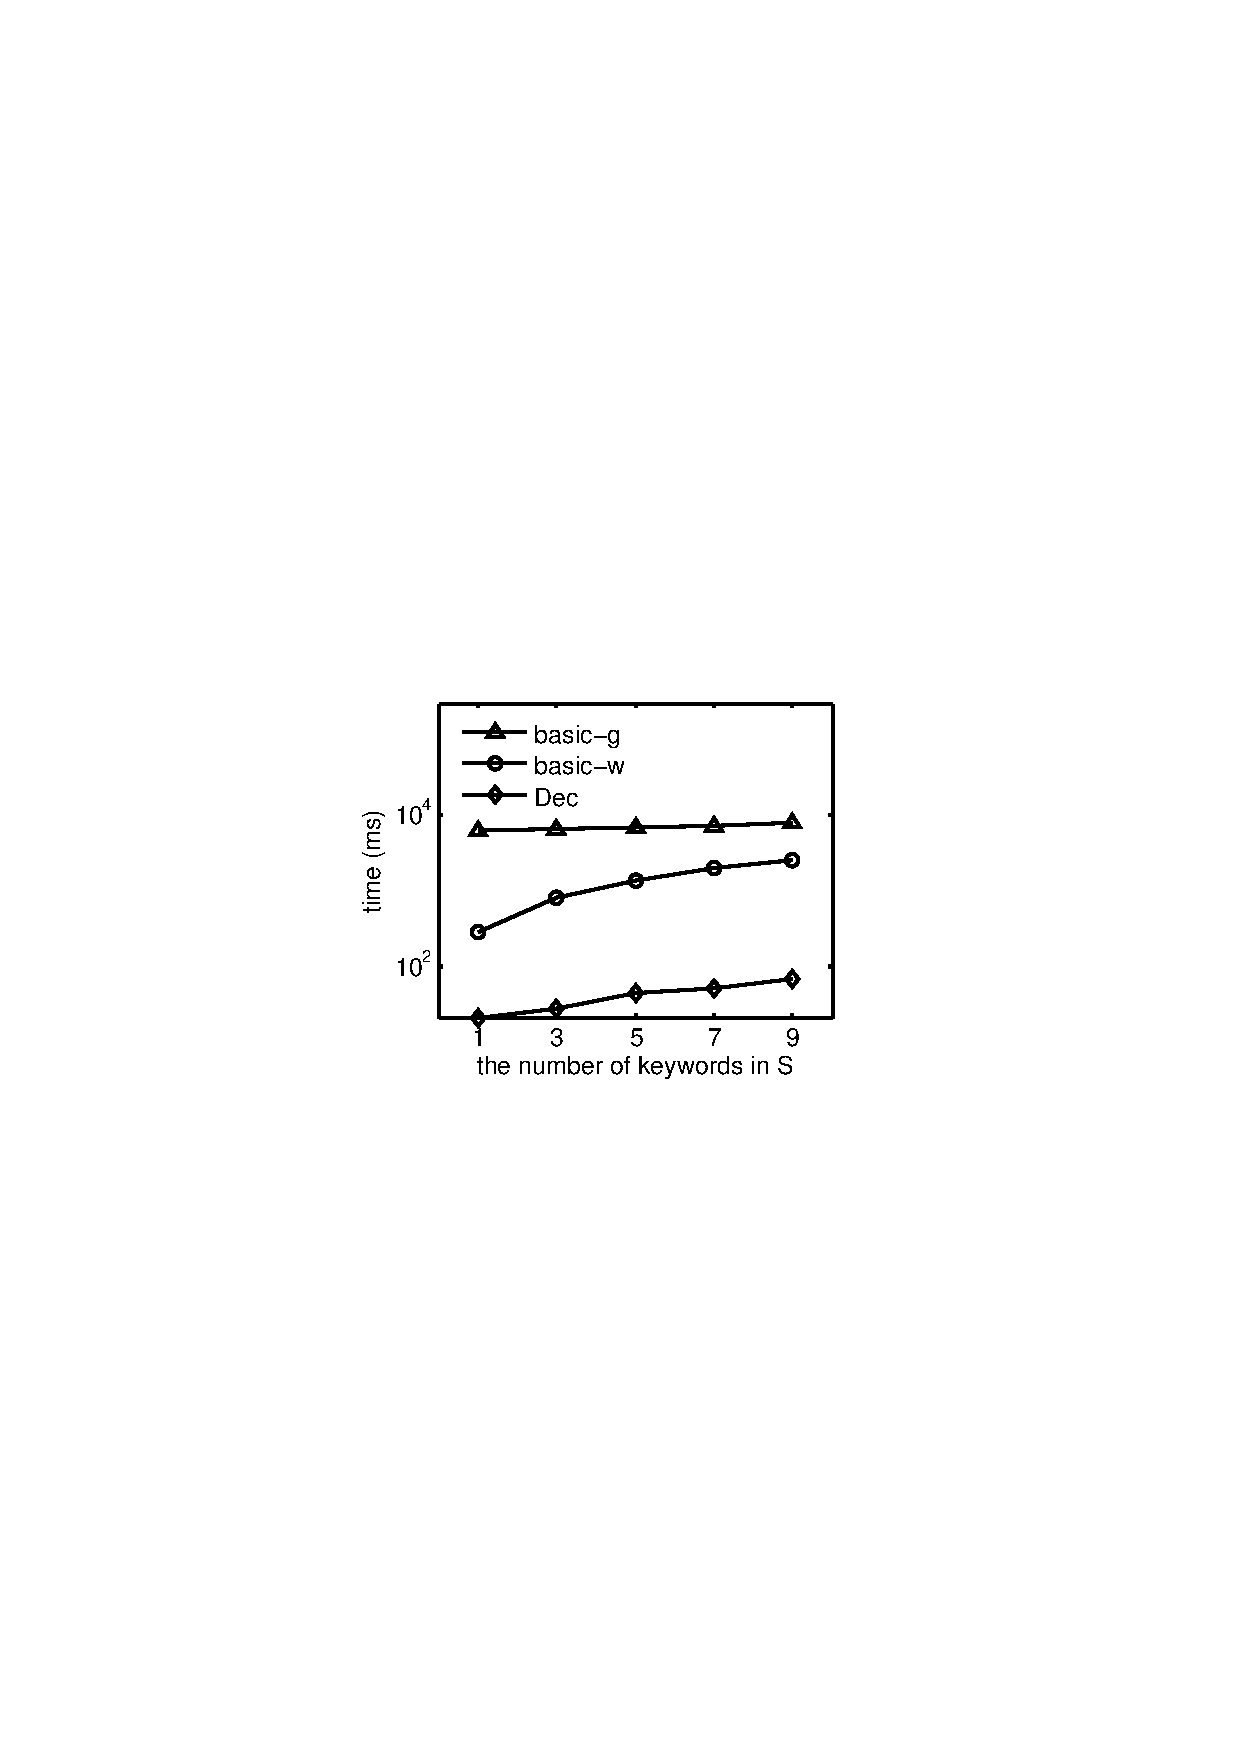
\includegraphics[width=3.725cm]{figures/tencent-s}
  \end{minipage}
  &
  \begin{minipage}{3.725cm}
	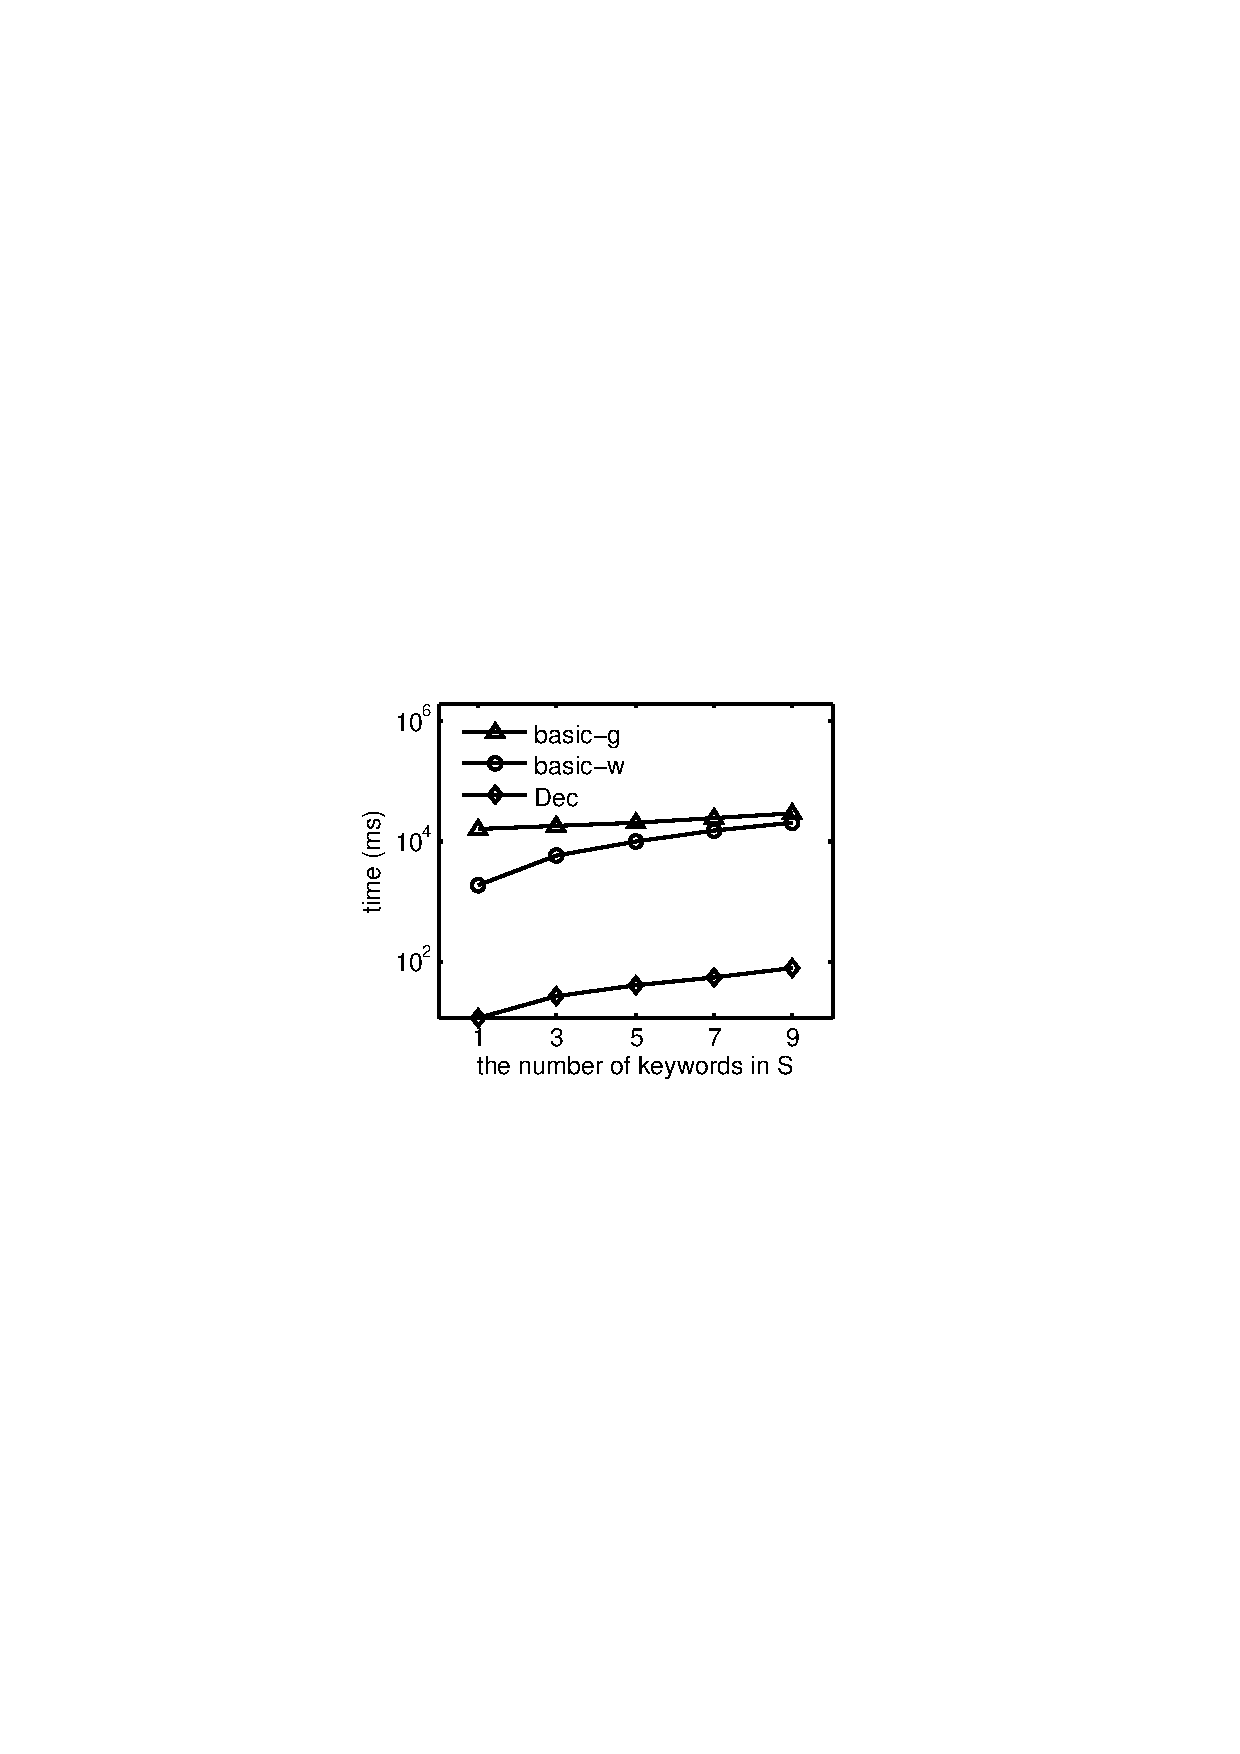
\includegraphics[width=3.725cm]{figures/dbpedia-s}
  \end{minipage}
  \\
  \small (q) Flickr (set $S$)
  &
  \small (r) DBLP (set $S$)
  &
  \small (s) Tencent (set $S$)
  &
  \small (t) DBpedia (set $S$)
 \end{tabular}
\caption{Efficiency results of community search.}
\label{fig:exp-problem1}
\end{figure*}

For each dataset, we randomly select 20\%, 40\%, 60\% and 80\%
of its vertices, and obtain four subgraphs induced by these vertex sets.
For each vertex, we randomly select 20\%, 40\%, 60\% and 80\%
of its keywords, and obtain four keyword sets.
%The results of index construction and ACQ evaluation are reported in Figures~\ref{fig:exp-index} and~\ref{fig:exp-problem1} respectively.

\textbf{1. Index construction.}
Figures~\ref{fig:exp-index}(a)-\ref{fig:exp-index}(d)
compare the efficiency of {\tt Basic} and {\tt Advanced}.
%Since their main difference is the part of building the tree structure, we also compare the parts of only building the tree without keywords.
We study their main parts, which build the tree without considering keywords.
We denote them by {\tt Basic-} and {\tt Advanced-}.
Notice that {\tt Advanced} performs consistently faster, and scales better, than {\tt Basic}.
When the subgraph size increases, the performance gap between {\tt Advanced} and {\tt Basic} is enlarged.
Similar results can be observed between {\tt Advanced-} and {\tt Basic-}.
In addition, we also run the CD method {\tt CODICIL}, which takes 32 mins, 2 mins, 1 day, and 3+ days (we stop it after runing 3 days) to cluster the vertices of Flickr, DBLP, Tencent and DBpedia offline respectively.

{\color{blue}
\textbf{2. Index Maintenance.}
We first evaluate the performance of keyword update and the results show that the keyword update is very fast. For example, inserting and deleting a keyword are around $10^6$ times faster than rebuilding the index.
Next, we show the performance of edge update on four static datasets in Figures~\ref{fig:exp-indexMaintenance}(a)-\ref{fig:exp-indexMaintenance}(h) by varying $k$.
In Figures~\ref{fig:exp-indexMaintenance}(a)-\ref{fig:exp-indexMaintenance}(b), we report the efficiency by separately performing edge insertion and deletion. Clearly, {\tt insertEdge} is $10^2$ to $10^5$ times faster than rebuilding index,
and {\tt deleteEdge} is also around $10^2$ times faster than rebuilding index.
The main reason is that, inserting or deleting one edge only affects a small proportion of CL-tree nodes and their connectivity.
In other words, most of the nodes remain unaffected.
Moreover, {\tt deleteEdge} is slower than {\tt insertEdge}. This is because, splitting tree nodes generally involves more computational cost than merging tree nodes.
In addition, we put all the insertion and deletion edges together, and report the efficiency by performing insertion and deletion for these edge with a random order. We report the results in Figures~\ref{fig:exp-indexMaintenance}(c)-\ref{fig:exp-indexMaintenance}(d),
where ``update" denote our algorithms including both {\tt insertEdge} and {\tt deleteEdge}.
We can see that, the index update algorithm is still much faster than rebuilding the index.

The results on real dynamic graphs (DFlickr and Youtube datasets) are shown in Figures~\ref{fig:exp-indexMaintenance}(i)-\ref{fig:exp-indexMaintenance}(j).
It is easy to observe that, the results on real dynamic graphs are similar to those on static graphs.
In summary, our proposed index maintenance algorithms are much faster than rebuilding the index from scratch.

%We can observe that the index maintenance algorithms are always much more efficient than rebuilding the CL-tree. In four static datasets, the curves of four real datasets are slightly different as the core number increases. For the edge insertion case, as shown in the Figure~\ref{fig:exp-indexMaintenance}(a)-\ref{fig:exp-indexMaintenance}(d), dynamically updating the tree index is $10^2$ to $10^5$ times faster than rebuilding the CL-tree. Note that our algorithms follows two main steps: (1) Compute vertices which may increase (decrease) the core numbers; (2) Update the tree index. And the reason for the phenomenon that it takes more time to as the core number increases, as shown in BDLP Figure~\ref{fig:exp-indexMaintenance}(b), is that the number of vertices whose core numbers range from 10 to 20 is relatively larger than others. As a result of that, we need to recursively compute the vertices which may increase the core numbers and, if necessary, update corresponding subtrees afterwards.
%
%For the edge deletion case, our index maintenance algorithm is around $10^2$ times faster than rebuilding. This is because besides computing vertices whose core numbers may decrease, after deleting an edge, the connectivity of vertices in one node is unknown, and therefore we have to reorganize all vetices in this node no matter what the core number is.
%
%In summary, as shown in the Figure~\ref{fig:exp-indexMaintenance}, dynamically updating edges is more efficient than rebuilding the tree from scratch. The trends of these curves reflect the scale and cohesiveness of vertices in real datasets. After the edge insertion or deletion, most parts of the tree remain unaffected and unchanged, and therefore the index dynamic maintenance is more effective and efficient.

}

\textbf{3. Efficiency of CS methods.}
Figures~\ref{fig:exp-problem1}(a)-\ref{fig:exp-problem1}(d) compares our best algorithm {\tt Dec} with existing CS methods. We see that {\tt Local} performs faster than {\tt Global} for most cases. Also, {\tt Dec}, which uses the CL-tree index, is the fastest.

\textbf{4. Effect of $k$.}
Figures~\ref{fig:exp-problem1}(e)-\ref{fig:exp-problem1}(h)
compare the query efficiency under different $k$.
A lower $k$ renders a larger subgraph, so as the time costs, for all the algorithms.
Note that {\tt basic-g} performs faster than {\tt basic-w}, but are slower than index-based algorithms.
{\tt Inc-T} performs better than {\tt Inc-S}, and {\tt Dec} performs the best.
The performance gaps decrease as $k$ increases.

\textbf{5. ACQ scalability w.r.t. keyword.}
Figures~\ref{fig:exp-problem1}(i)-\ref{fig:exp-problem1}(l) examine scalability over the fraction of keywords for each vertex. All the vertices are considered. The running times of the algorithms increase as more keywords are involved. {\tt Dec} performs the best.

\textbf{6. ACQ scalability w.r.t. vertex.}
Figures~\ref{fig:exp-problem1}(m)-\ref{fig:exp-problem1}(p) report the scalability over different fraction of vertices.
All the keywords of each vertex are considered. Again, {\tt Dec} scales the best.

\textbf{7. Effect of size of $S$.}
For each query vertex, we randomly select 1, 3, 5, 7 and 9 keywords to form the query keyword set $S$.
As {\tt Dec} performs better than {\tt Inc-S} and {\tt Inc-T}, we mainly compare {\tt Dec} with the baseline solutions. Figures~\ref{fig:exp-problem1}(q)-\ref{fig:exp-problem1}(t) show that the cost of all algorithms increase with the $|S|$. Also, {\tt Dec} is 1 to 3 order-of-magnitude faster than {\tt basic-g} and {\tt basic-w}.

\begin{figure*}[htb]
\setlength{\abovecaptionskip}{0.cm}
\setlength{\belowcaptionskip}{-1cm}
\hspace*{-.4cm}
\centering
\begin{tabular}{c c c c}
  \begin{minipage}{3.36cm}
	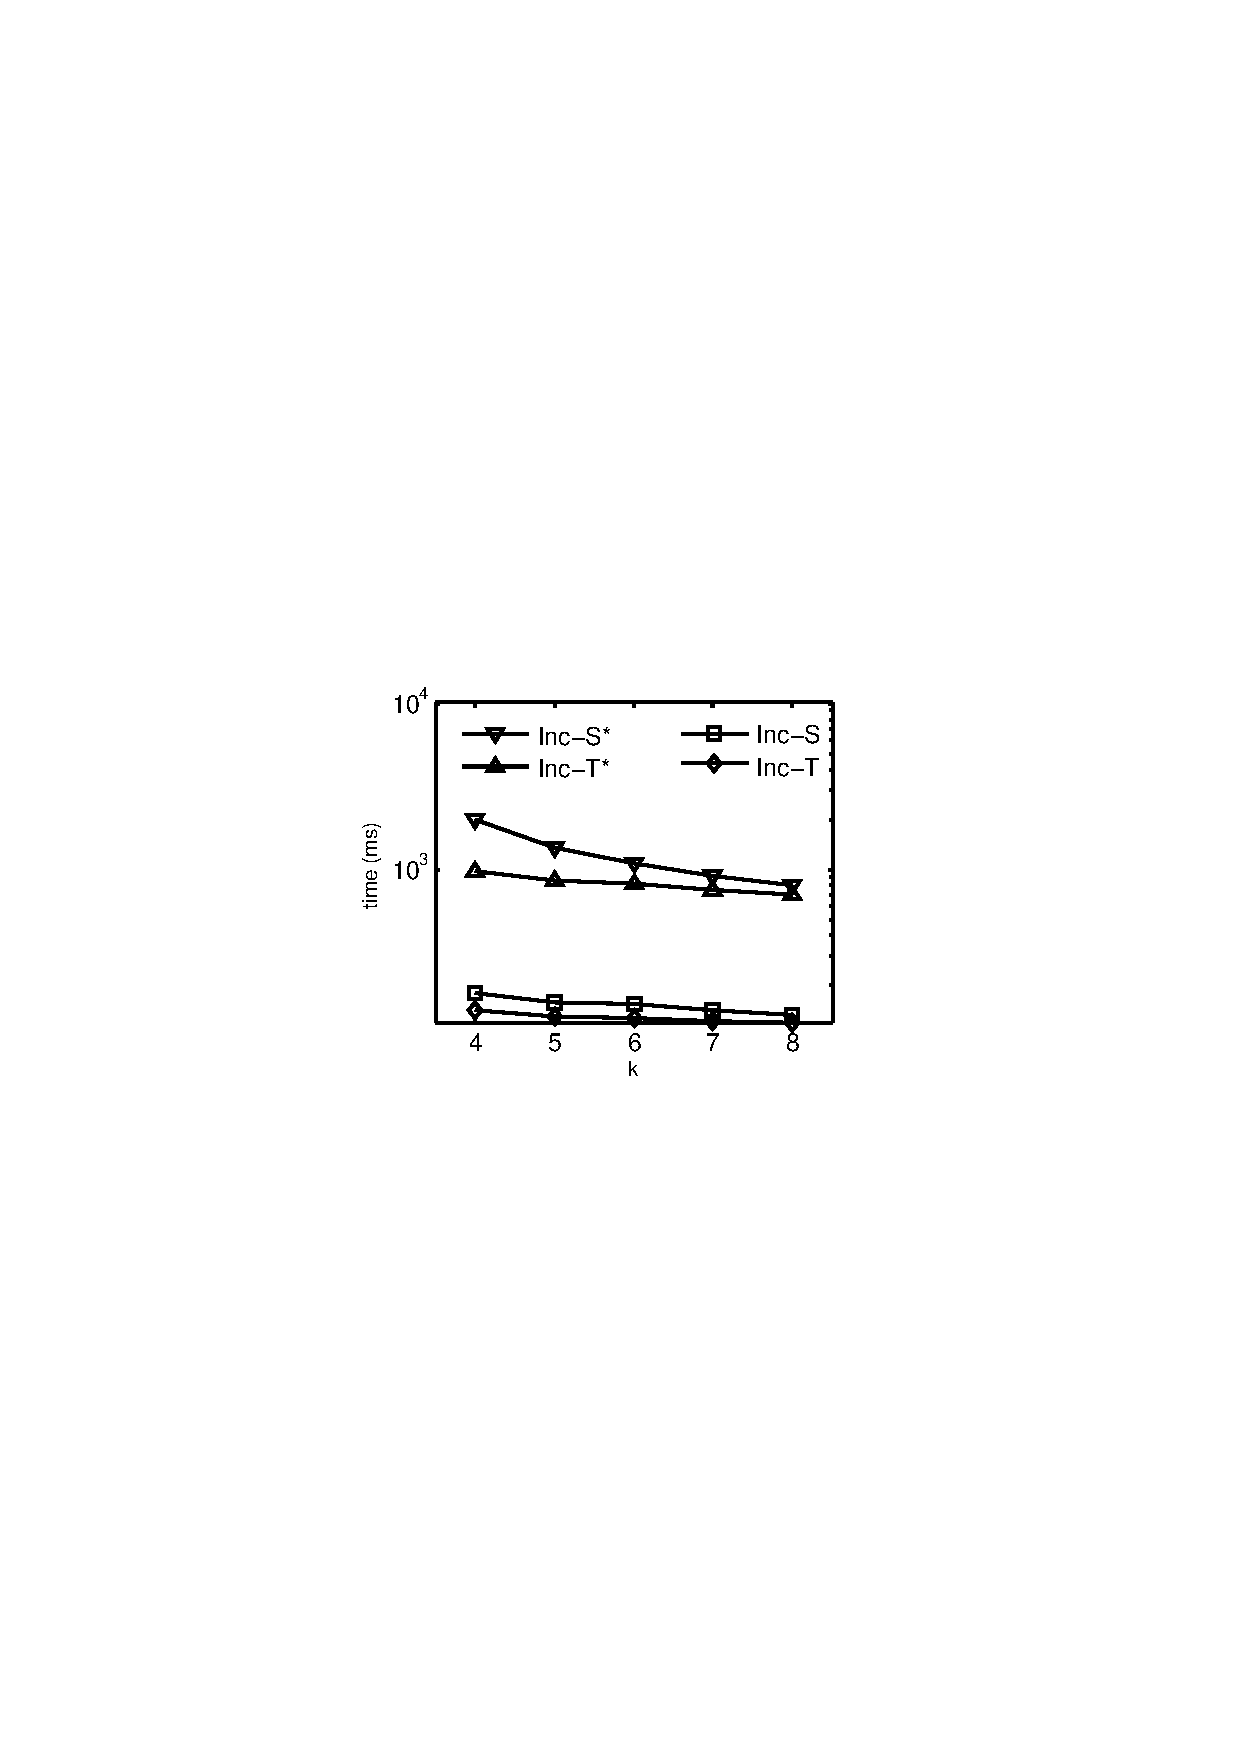
\includegraphics[width=3.325cm]{figures/flickrInverted}
  \end{minipage}
  &
  \begin{minipage}{3.36cm}
	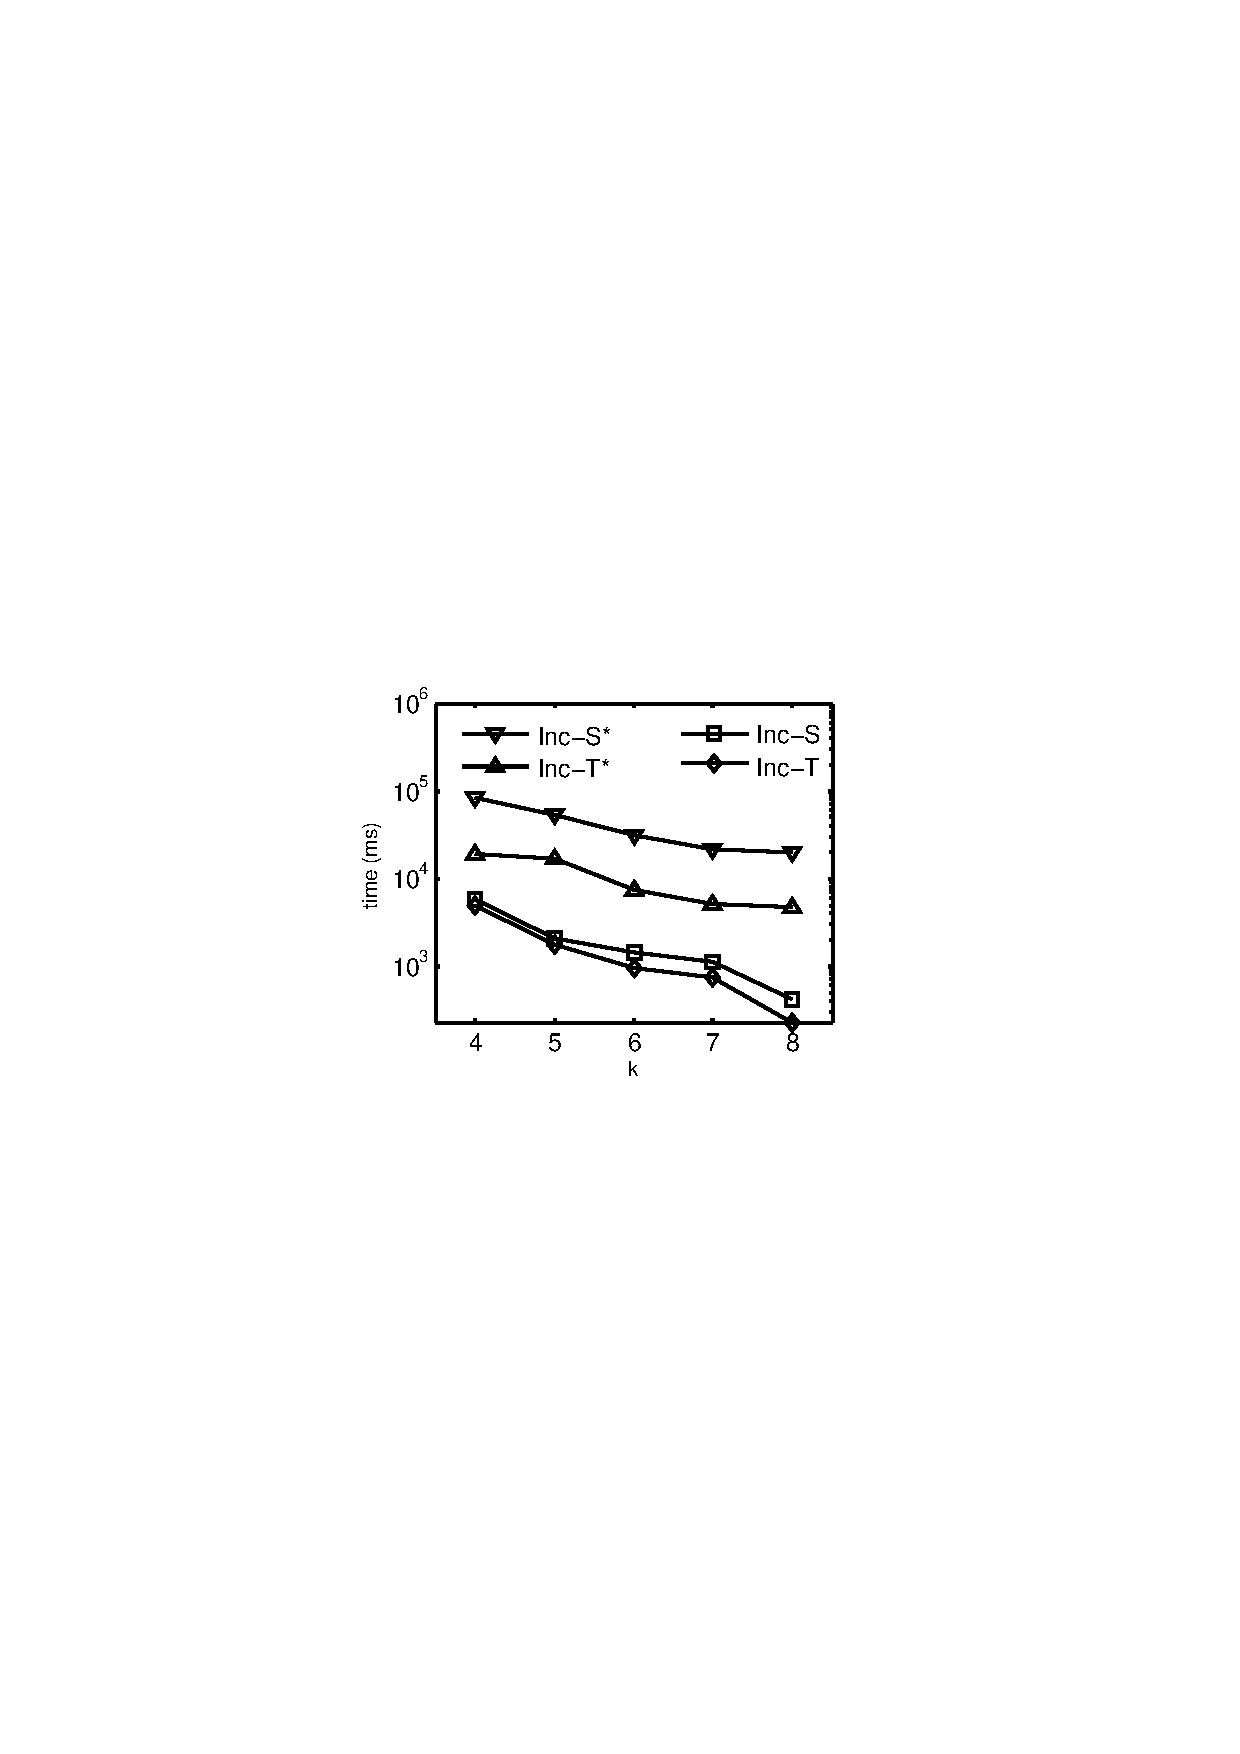
\includegraphics[width=3.325cm]{figures/dblpInverted}
  \end{minipage}
  &
  \begin{minipage}{3.36cm}
	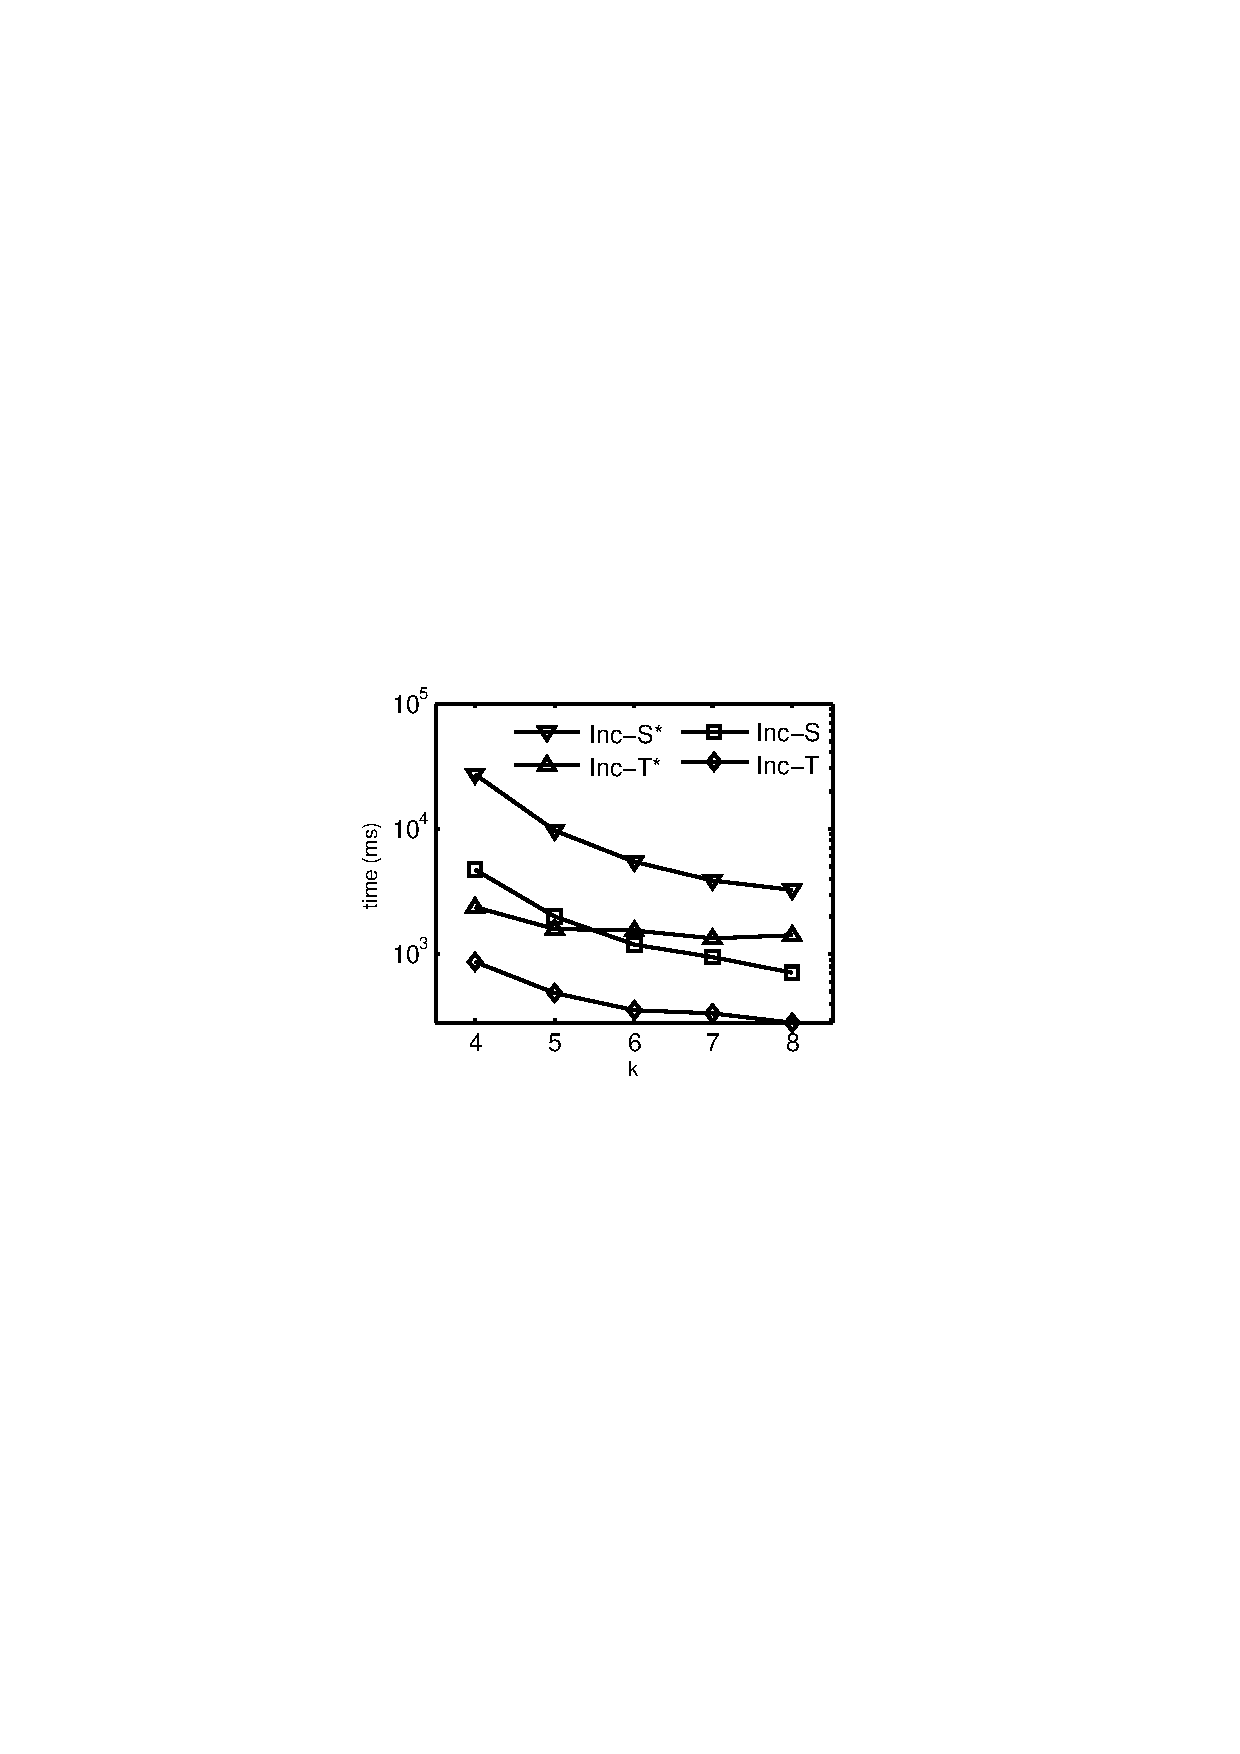
\includegraphics[width=3.325cm]{figures/tencentInverted}
  \end{minipage}
  &
  \begin{minipage}{3.36cm}
	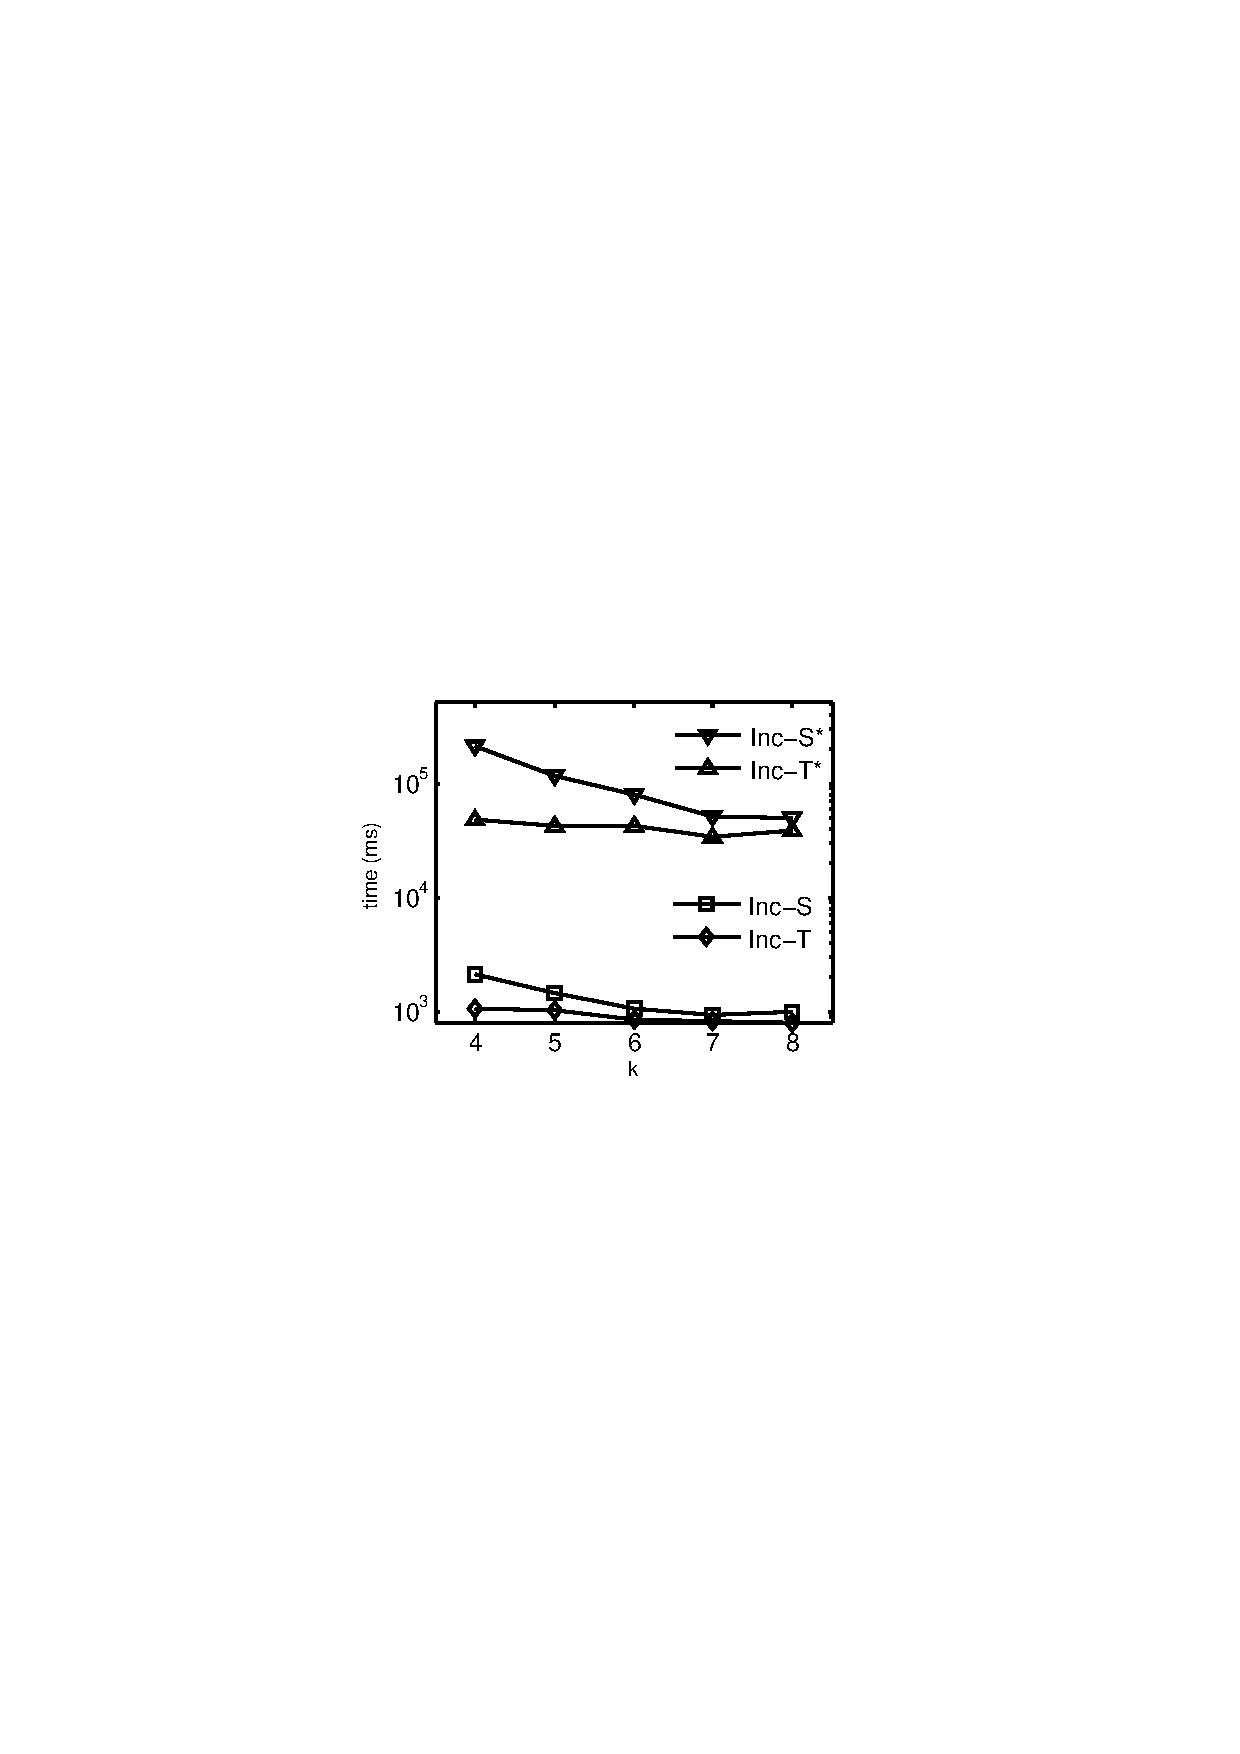
\includegraphics[width=3.325cm]{figures/dbpediaInverted}
  \end{minipage}
  \\
  \small (a) Flickr
  &
  \small (b) DBLP
  &
  \small (c) Tencent
  &
  \small (d) DBpedia
\end{tabular}
\caption{Effect of InvertedList for {\tt Inc-S} and {\tt Inc-T}.}
\label{fig:exp-more-inverted}
\end{figure*}

\begin{figure*}[htb]
\setlength{\abovecaptionskip}{0.cm}
\setlength{\belowcaptionskip}{-1cm}
\hspace*{-.4cm}
\centering
\begin{tabular}{c c c c}
  \begin{minipage}{3.36cm}
	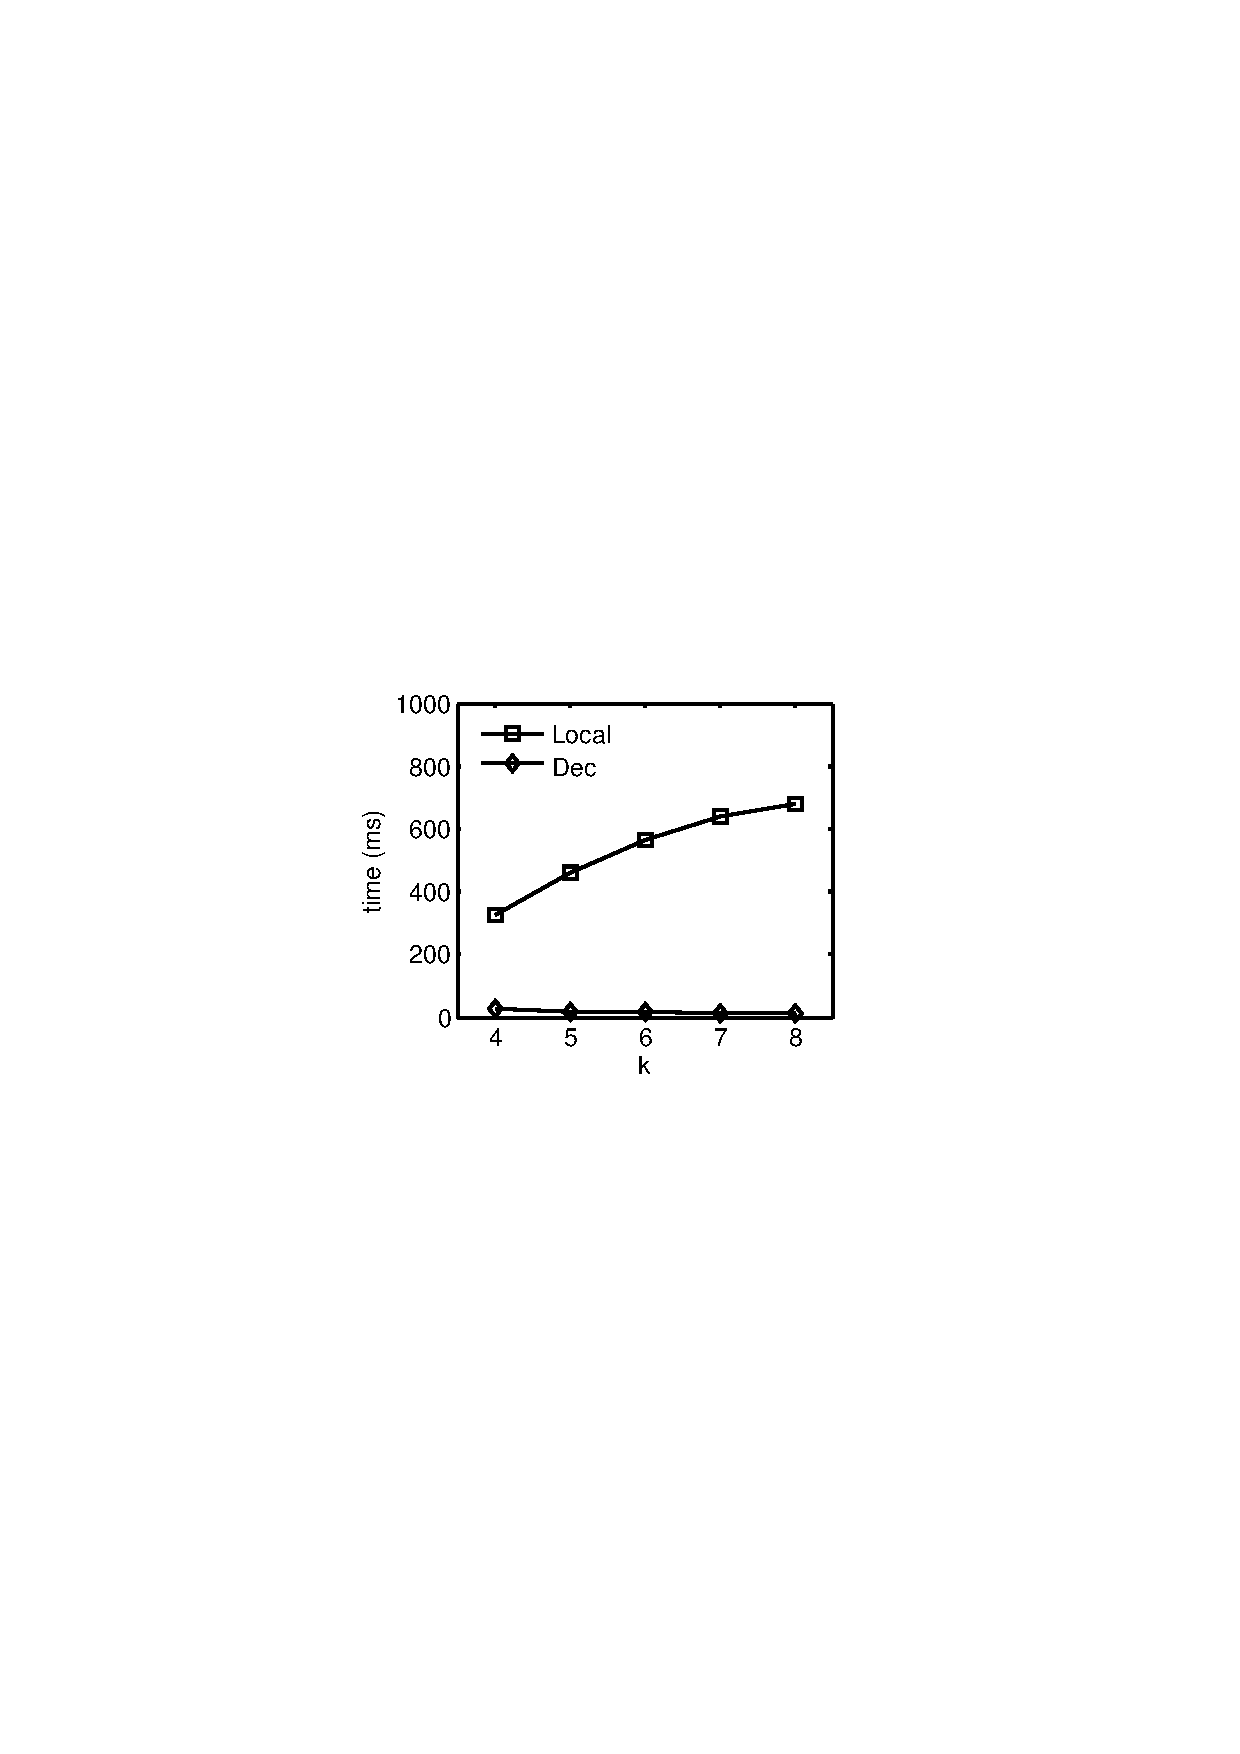
\includegraphics[width=3.325cm]{figures/flickrDecComp}
  \end{minipage}
  &
  \begin{minipage}{3.36cm}
	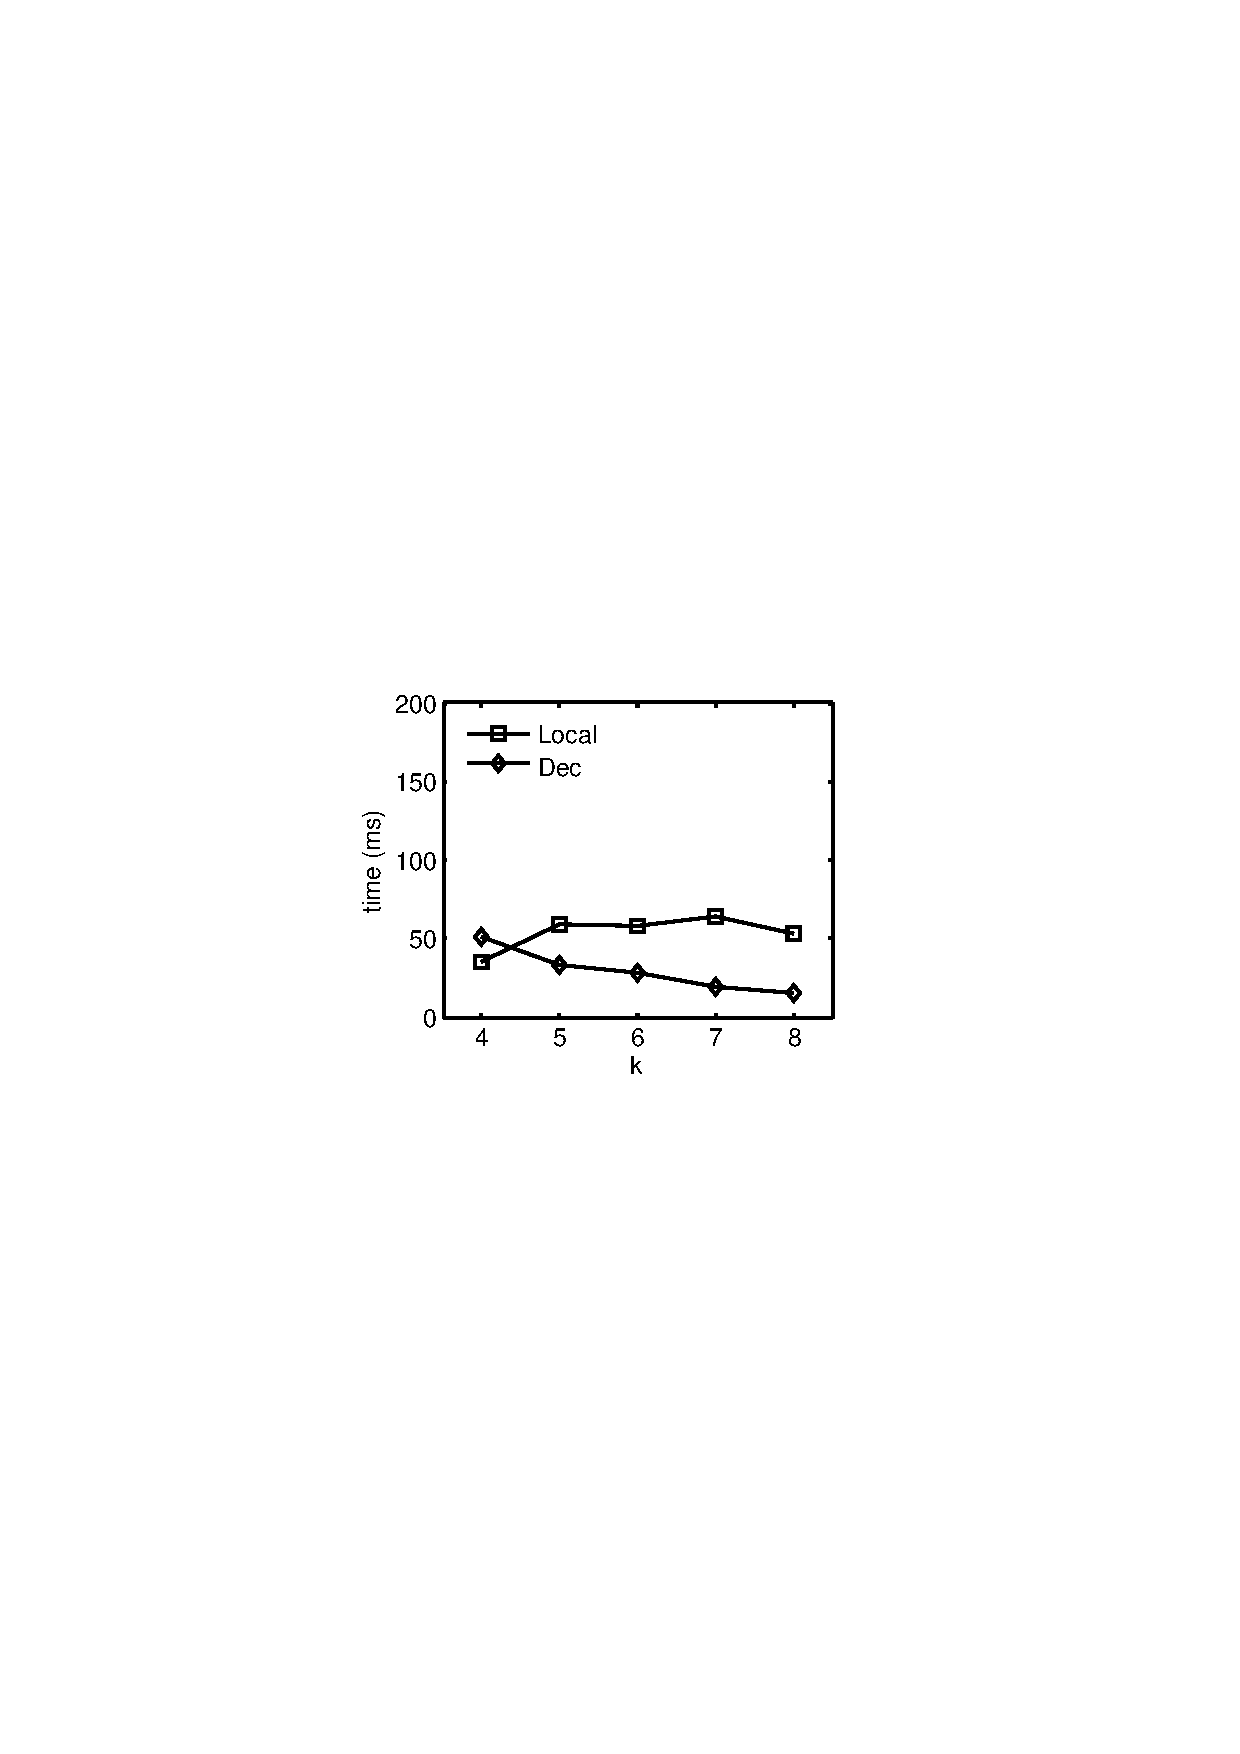
\includegraphics[width=3.325cm]{figures/dblpDecComp}
  \end{minipage}
  &
  \begin{minipage}{3.36cm}
	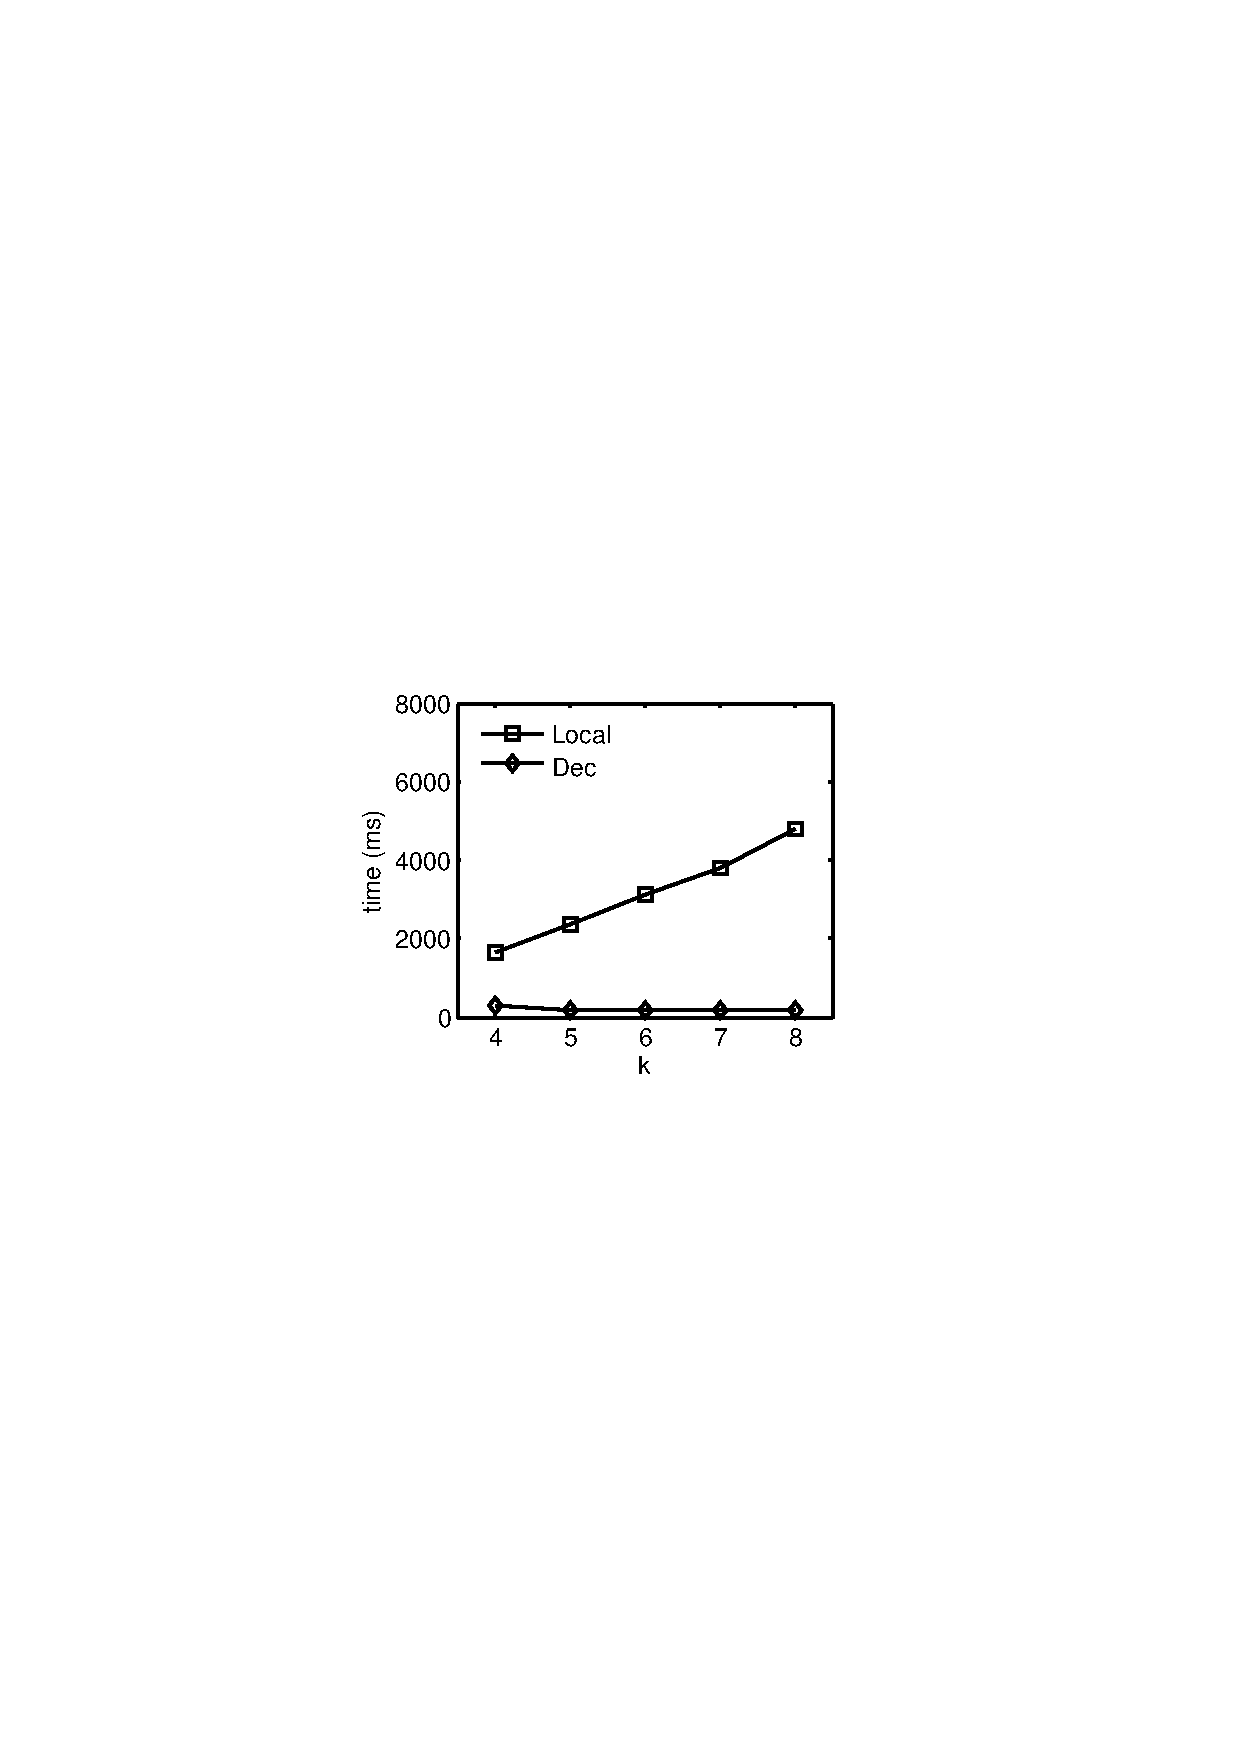
\includegraphics[width=3.325cm]{figures/tencentDecComp}
  \end{minipage}
  &
  \begin{minipage}{3.36cm}
	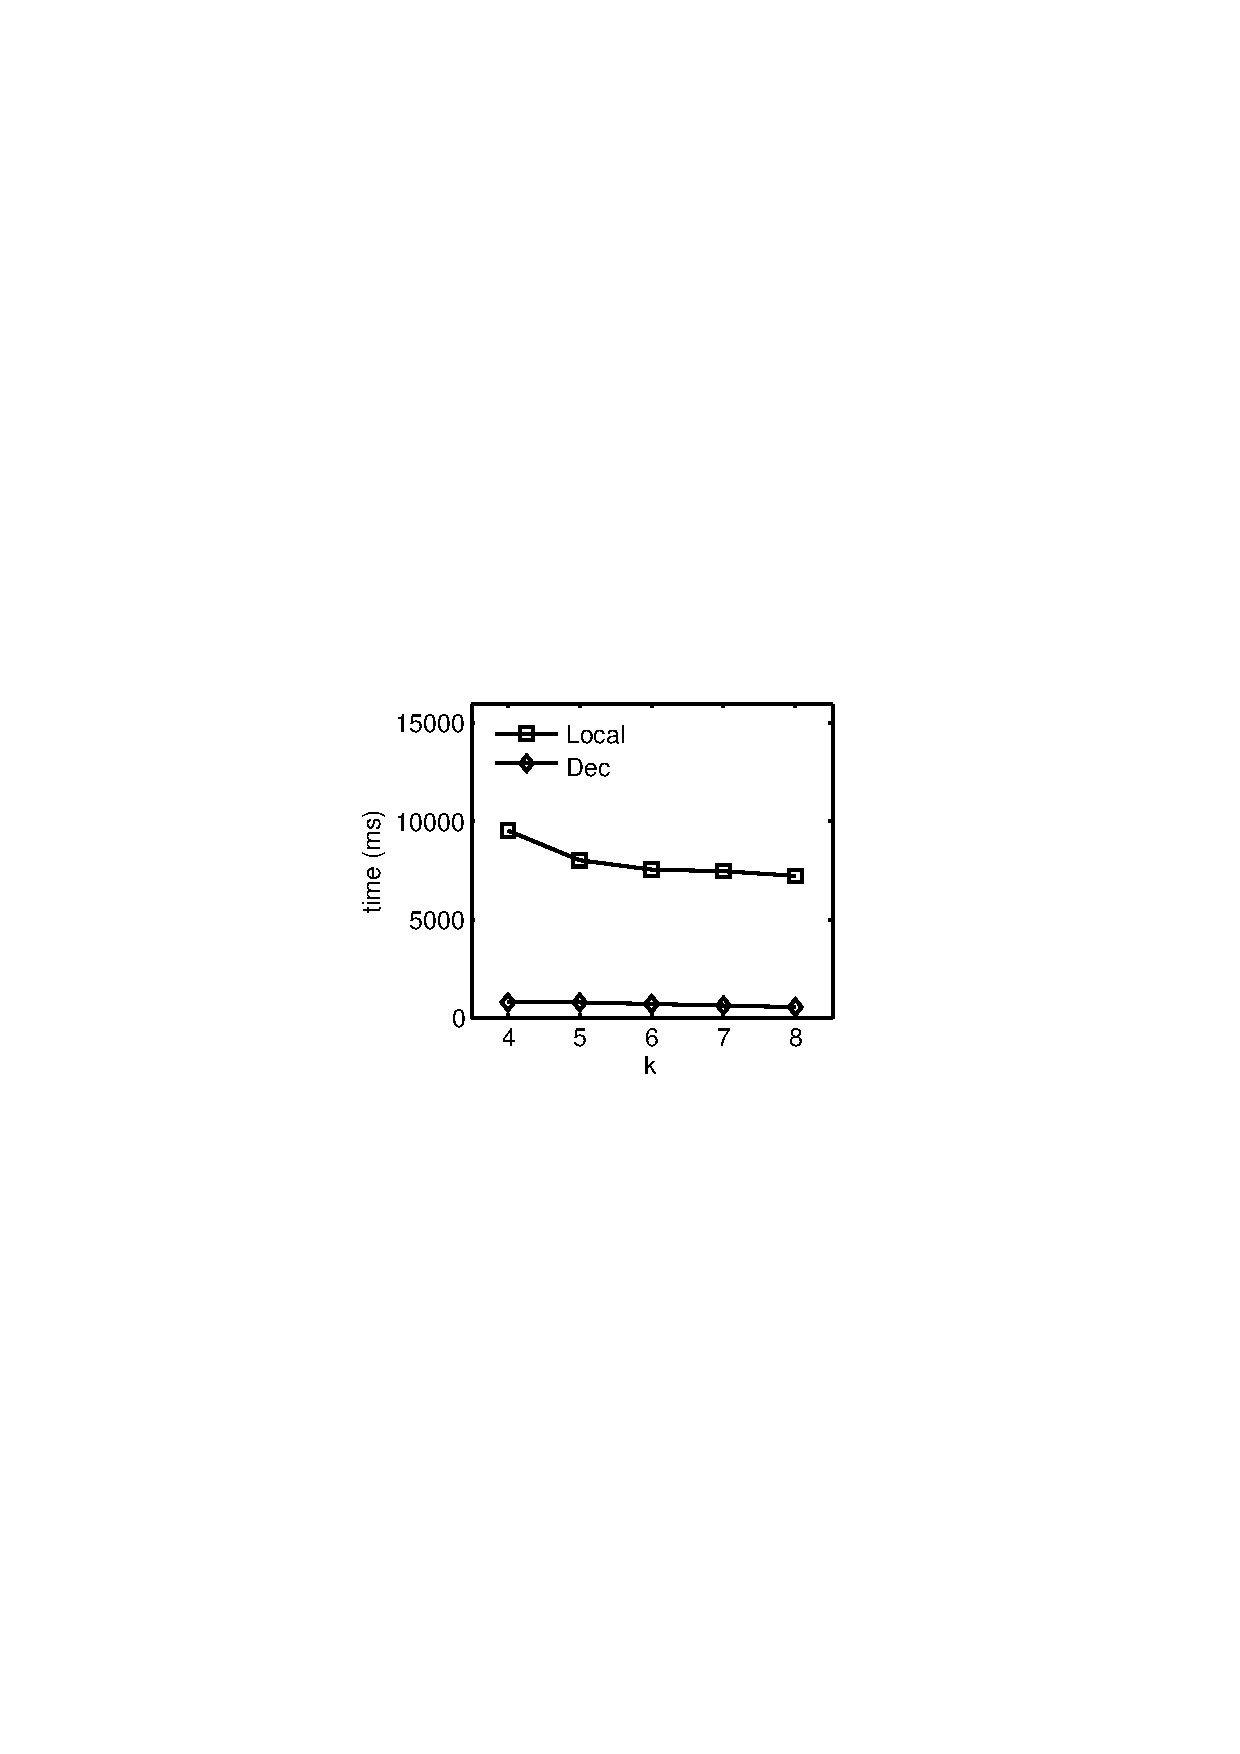
\includegraphics[width=3.325cm]{figures/dbpediaDecComp}
  \end{minipage}
  \\
  \small (a) Flickr
  &
  \small (b) DBLP
  &
  \small (c) Tencent
  &
  \small (d) DBpedia
\end{tabular}
\caption{Results on non-attributed graphs.}
\label{fig:exp-more-decComp}
\end{figure*}



\begin{figure*}[htb]
\hspace*{-.4cm}
\centering
\begin{tabular}{c c c c}
  \begin{minipage}{3.325cm}
  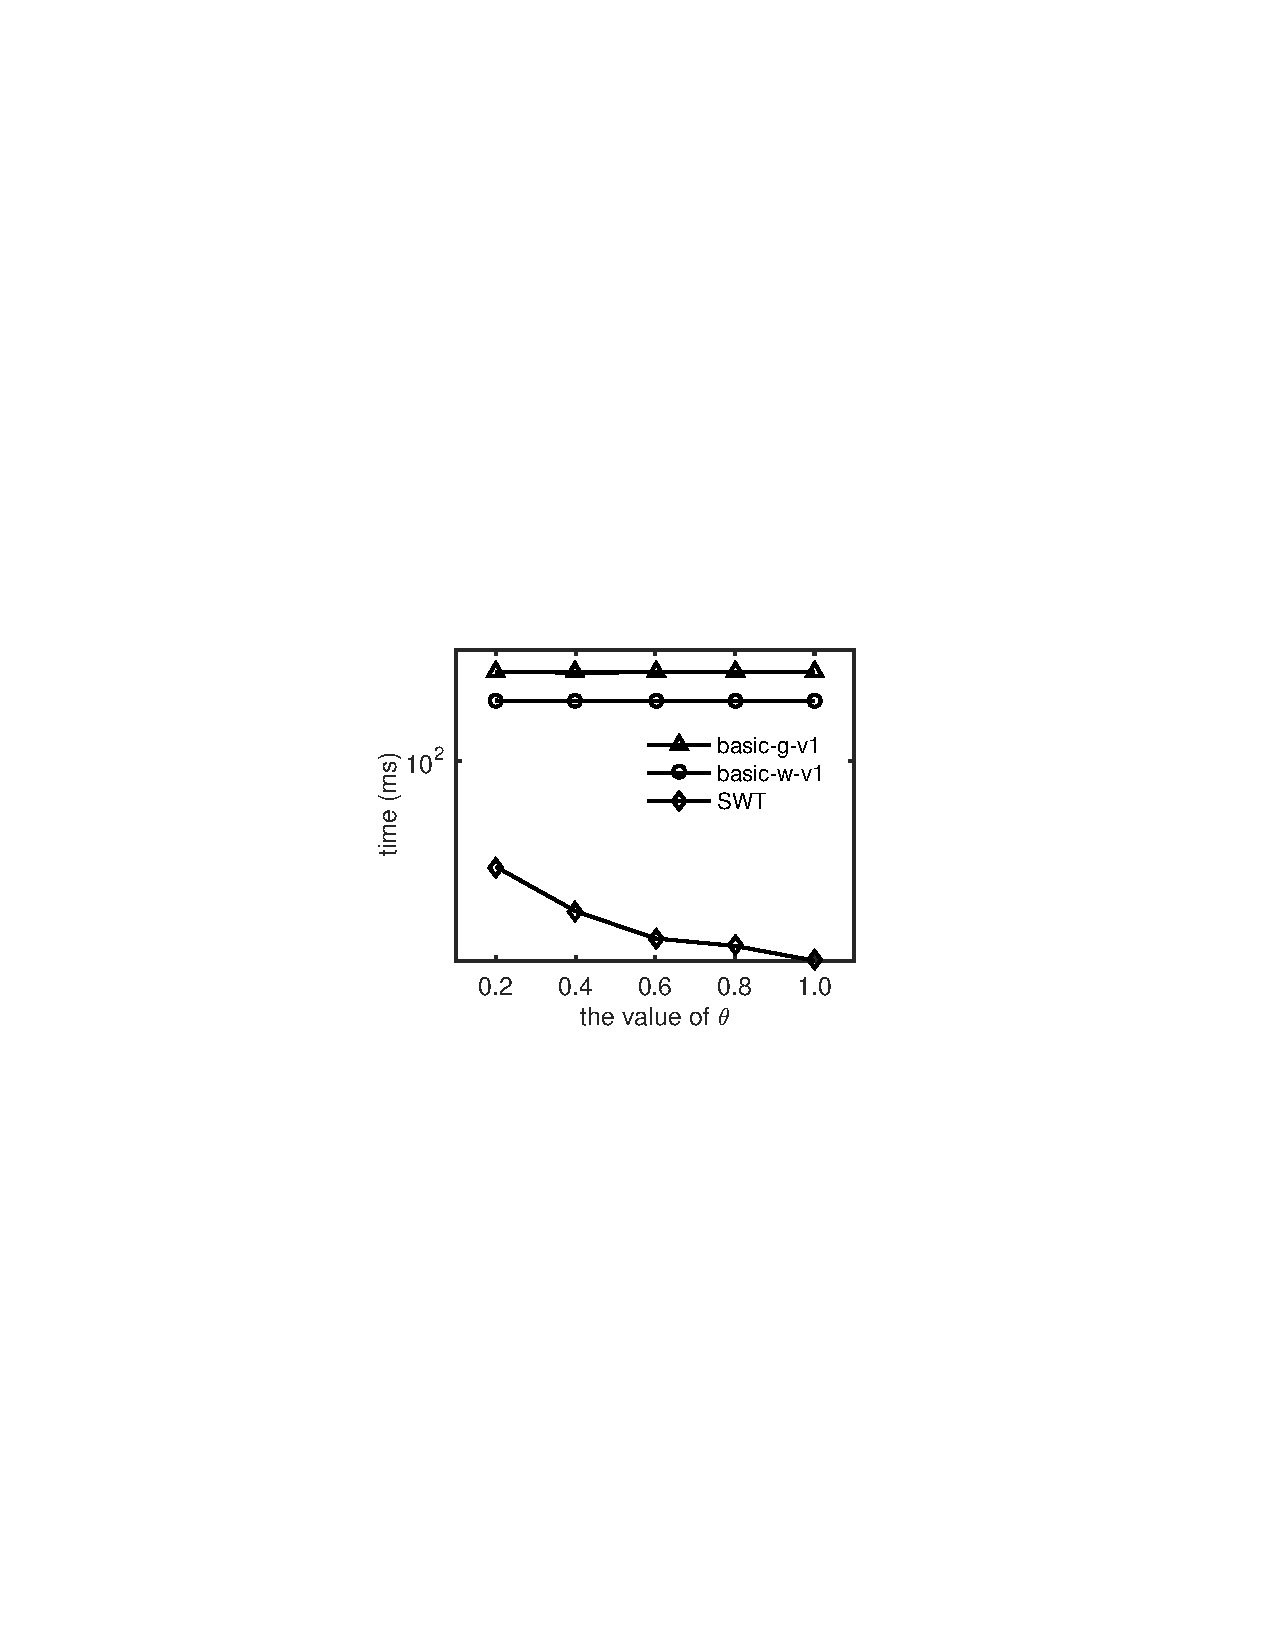
\includegraphics[width=3.725cm]{figures/flickrv1}
  \end{minipage}
  &
  \begin{minipage}{3.325cm}
  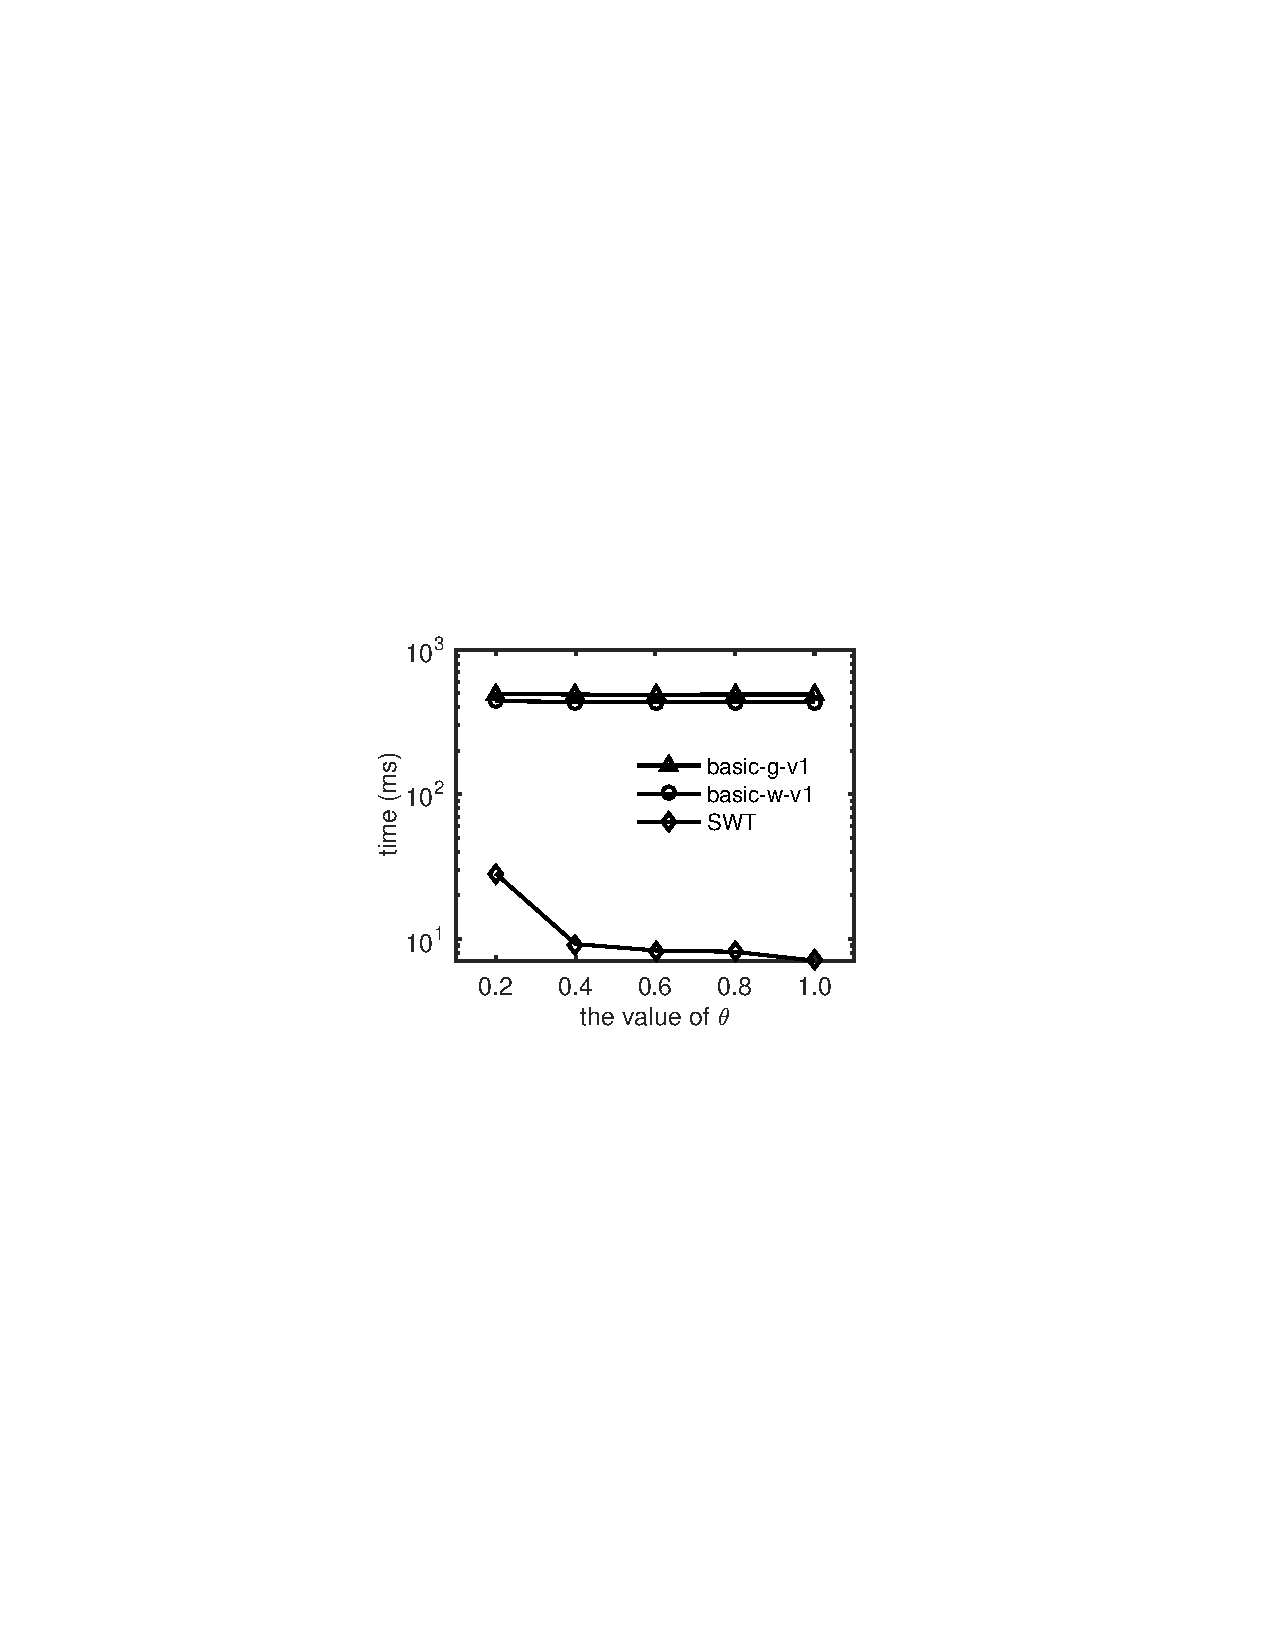
\includegraphics[width=3.725cm]{figures/dblpv1}
  \end{minipage}
  &
  \begin{minipage}{3.325cm}
  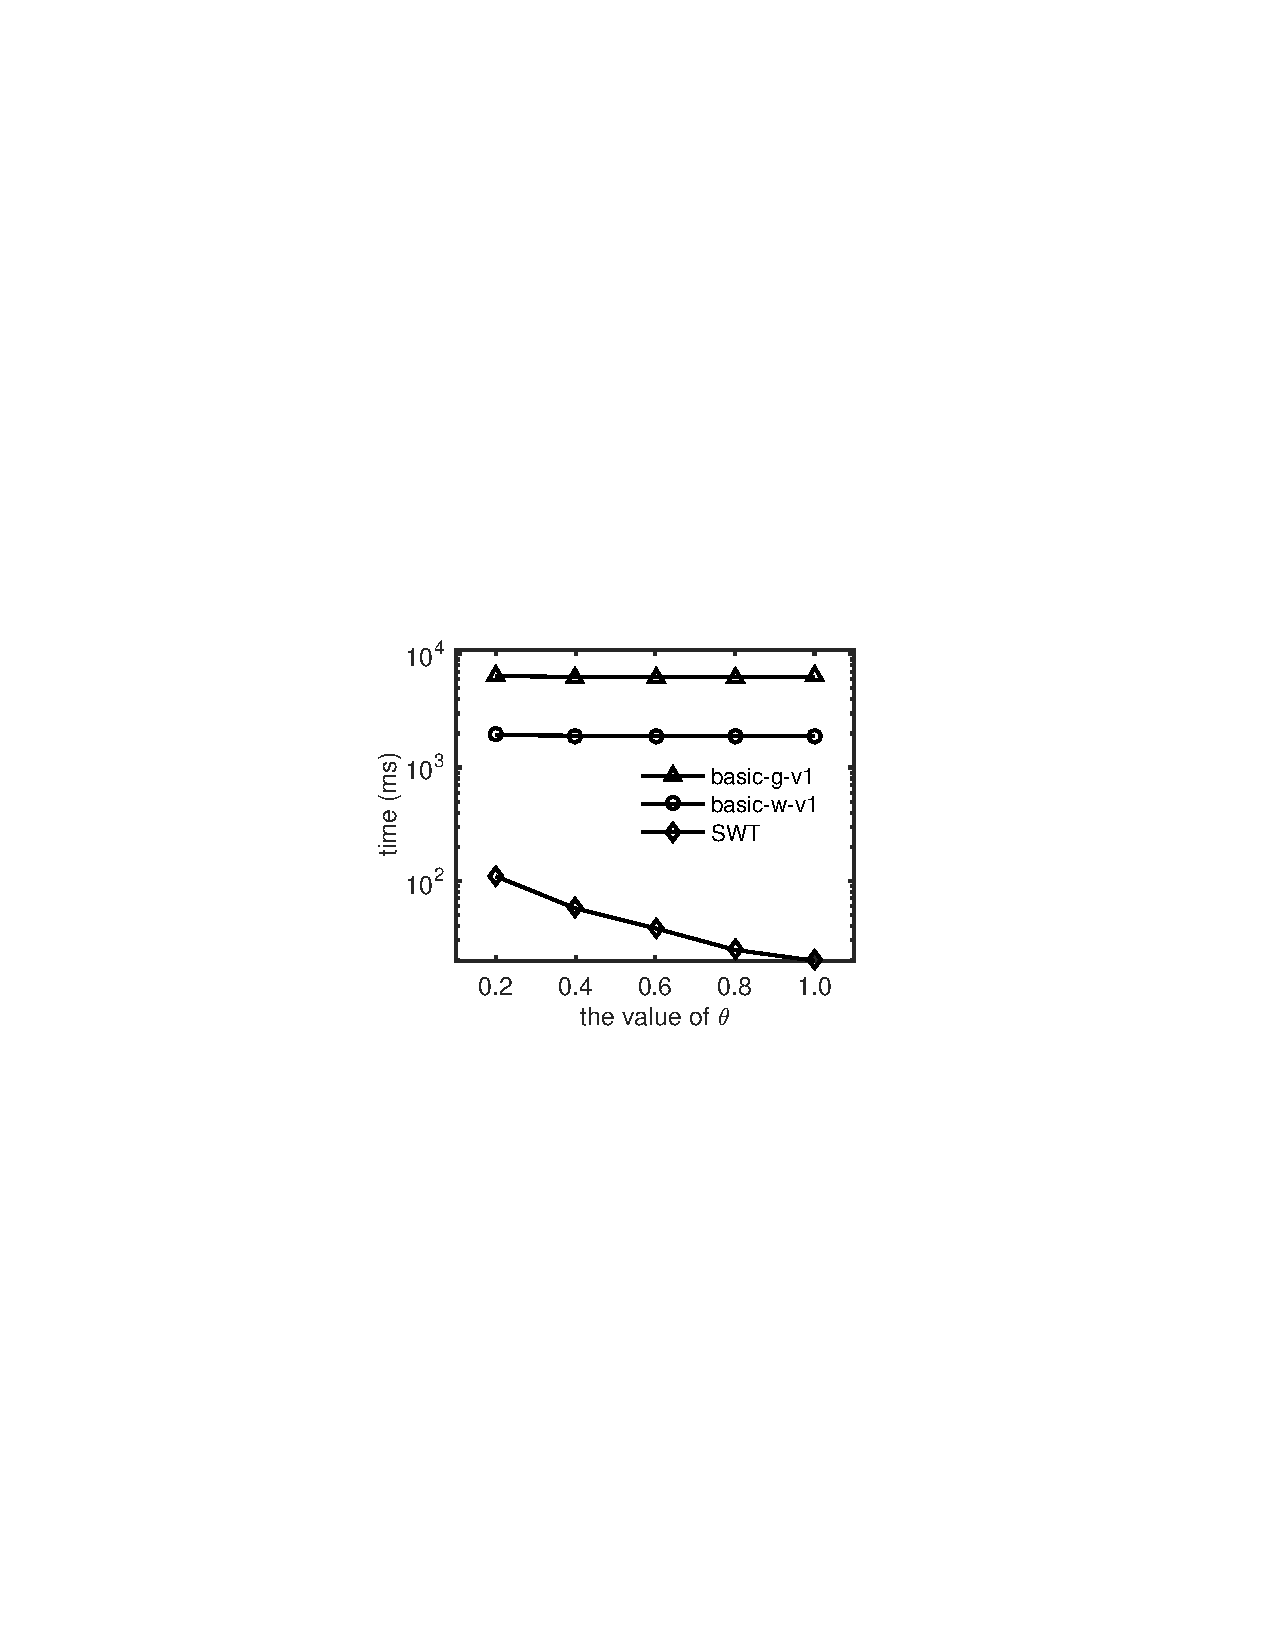
\includegraphics[width=3.725cm]{figures/tencentv1}
  \end{minipage}
  &
  \begin{minipage}{3.325cm}
  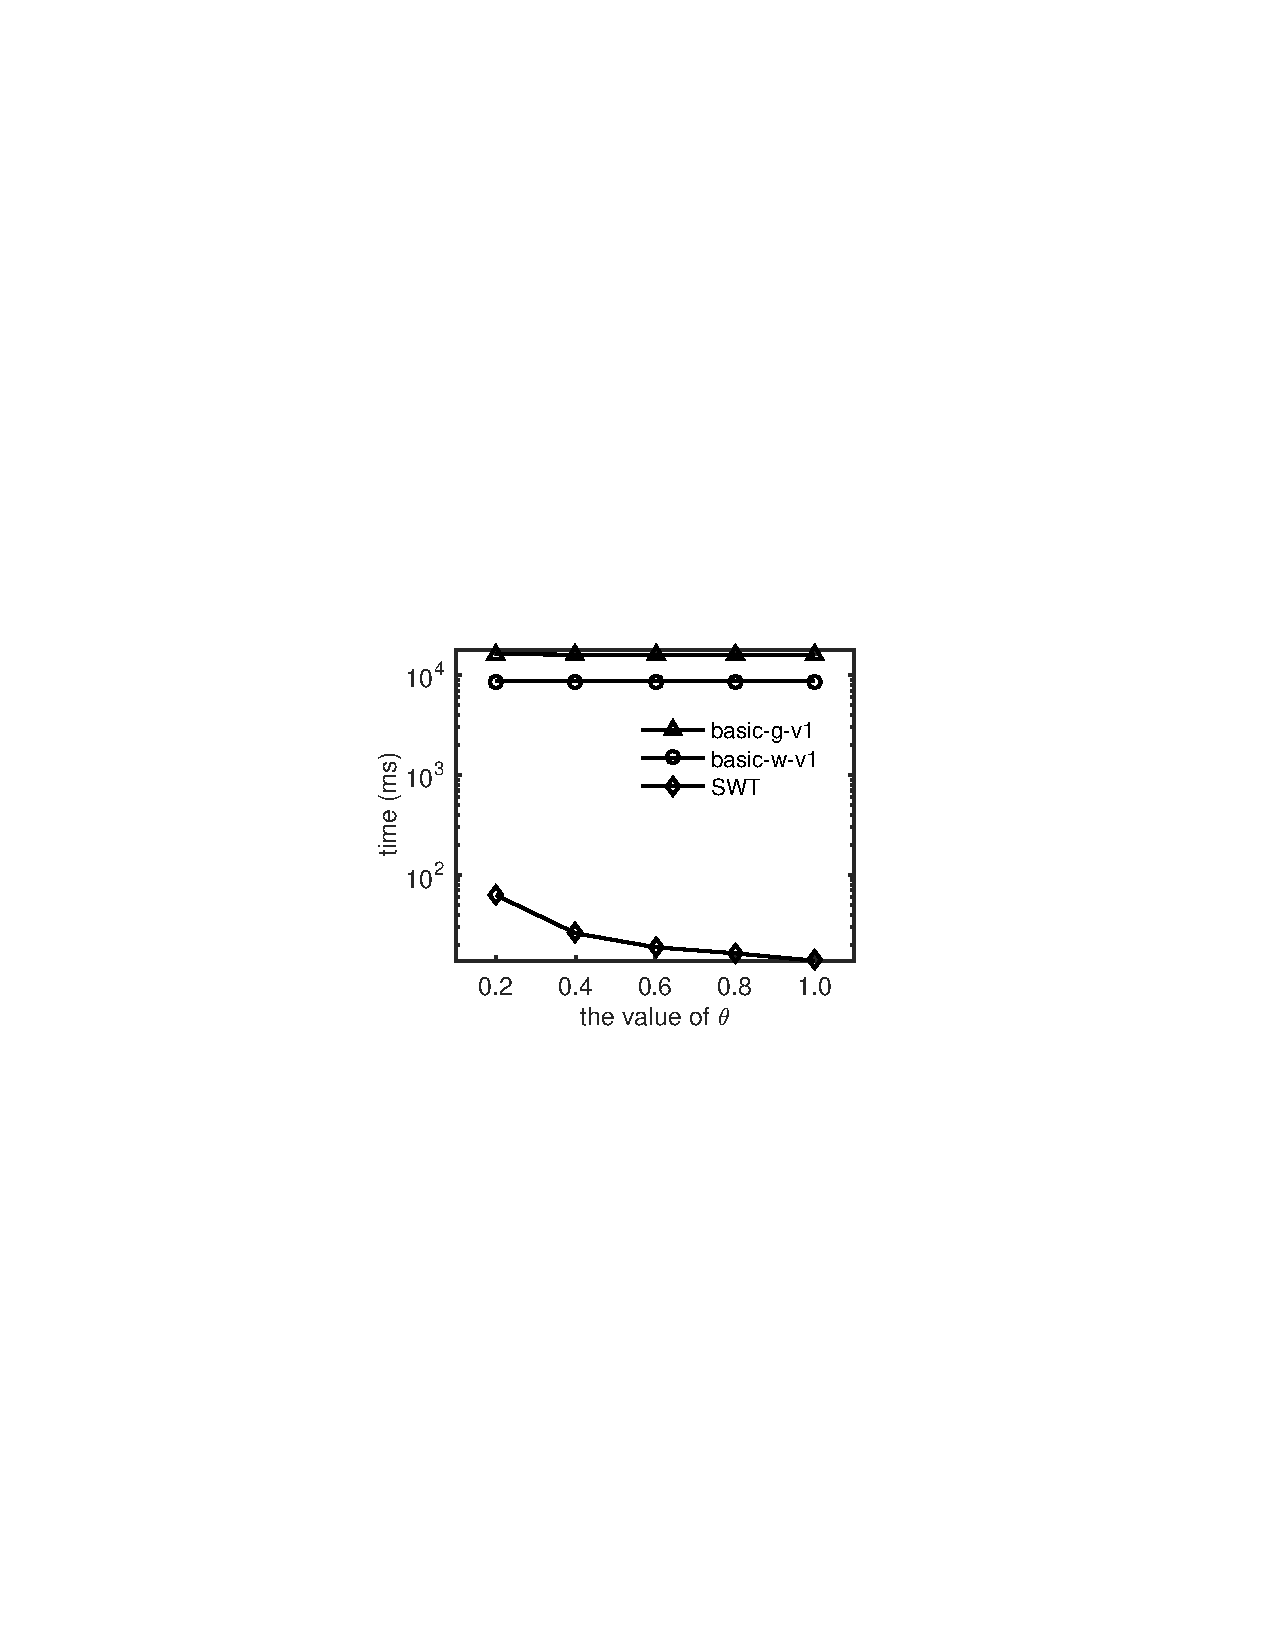
\includegraphics[width=3.725cm]{figures/dbpediav1}
  \end{minipage}
  \\
  \small (a) Flickr (Variant 1)
  &
  \small (b) DBLP (Variant 1)
  &
  \small (c) Tencent (Variant 1)
  &
  \small (d) DBpedia (Variant 1)
      \\
  \begin{minipage}{3.325cm}
  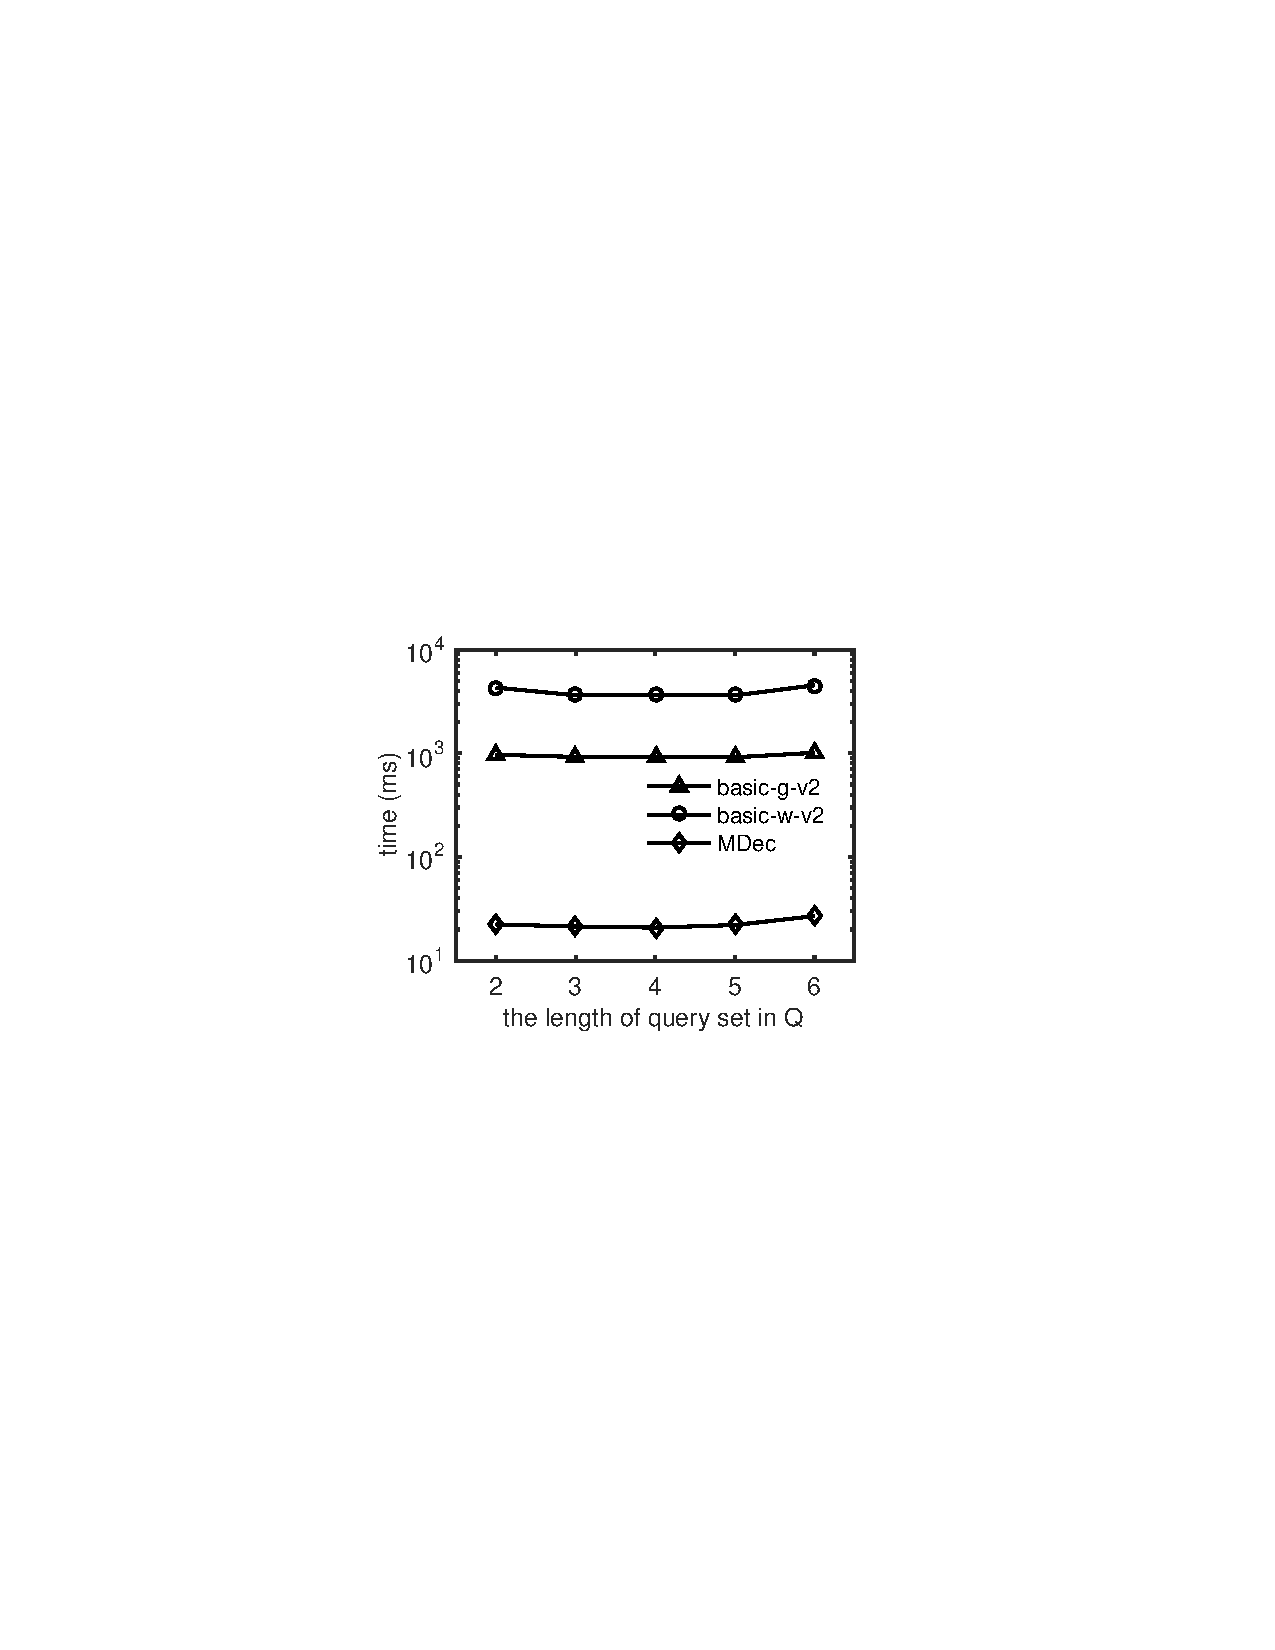
\includegraphics[width=3.725cm]{figures/flickrv2}
  \end{minipage}
  &
  \begin{minipage}{3.325cm}
  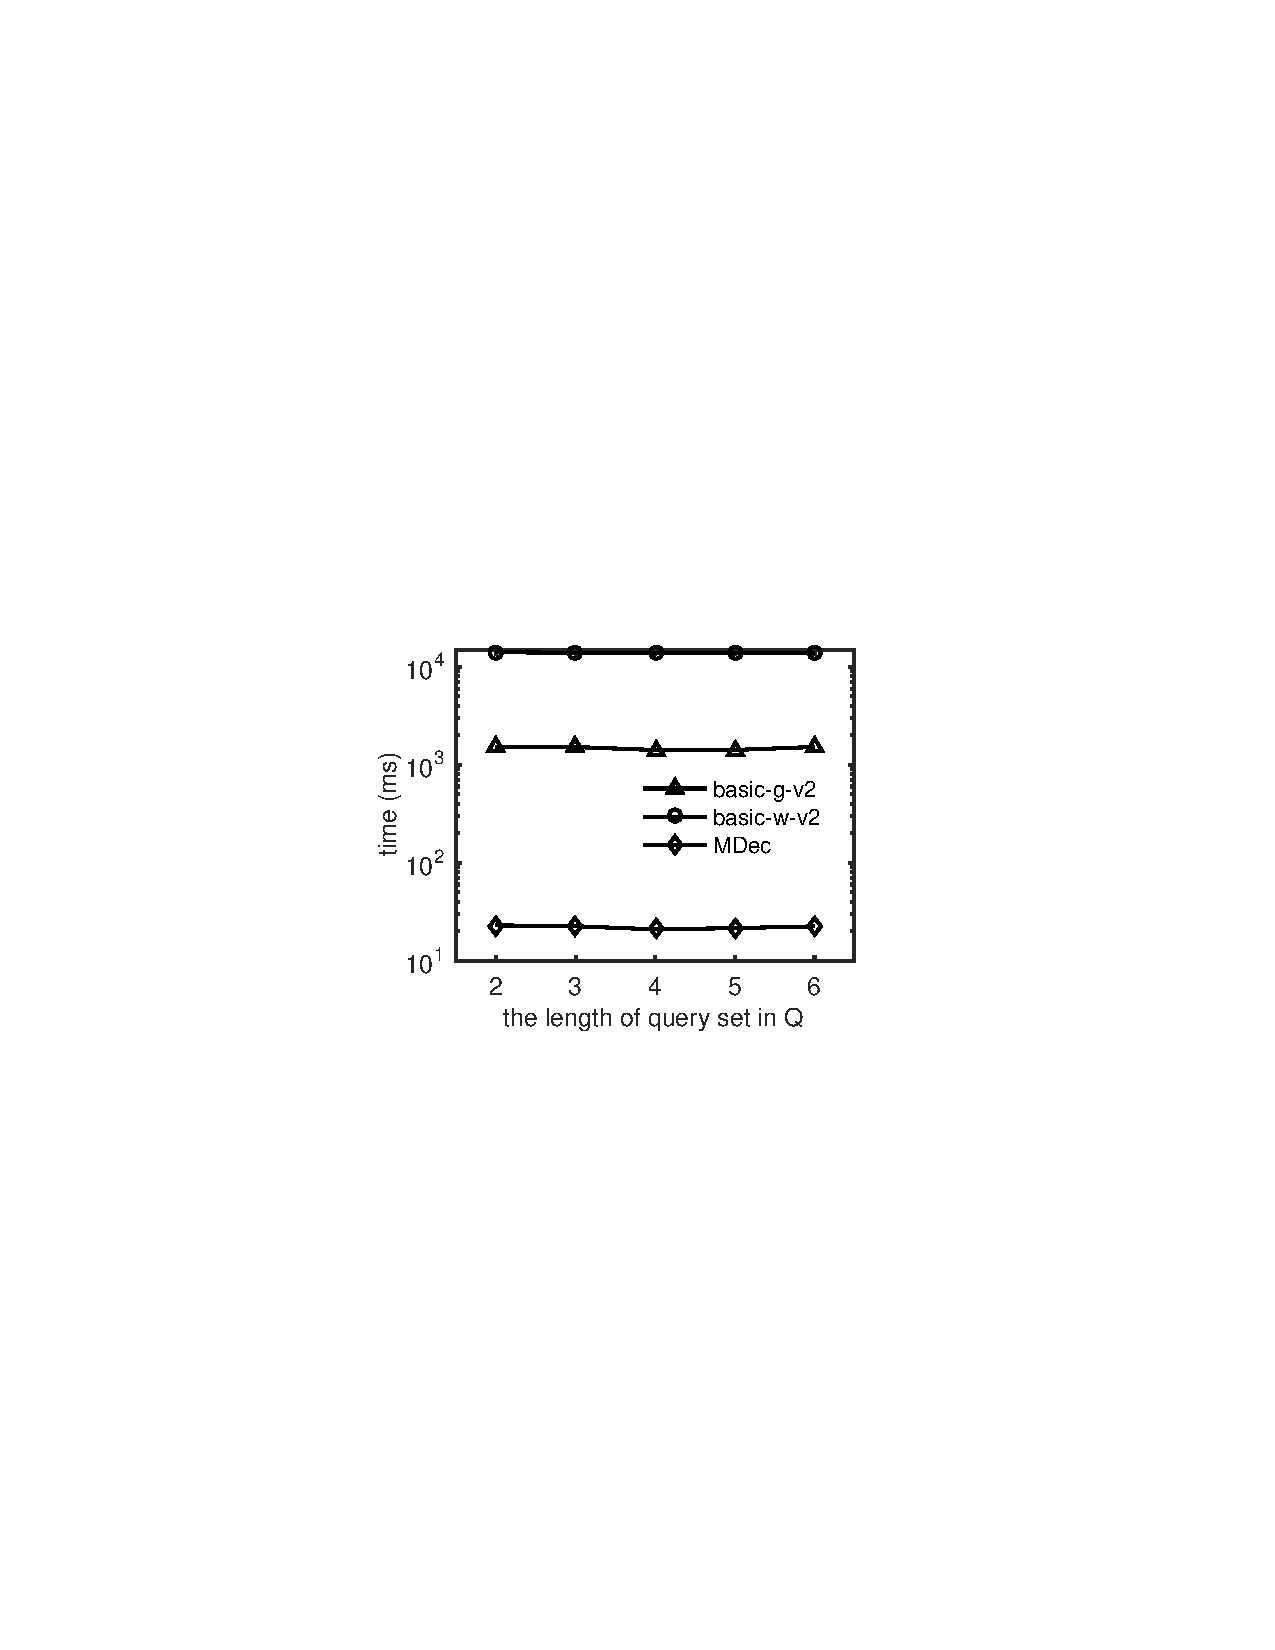
\includegraphics[width=3.725cm]{figures/dblpv2}
  \end{minipage}
  &
  \begin{minipage}{3.325cm}
  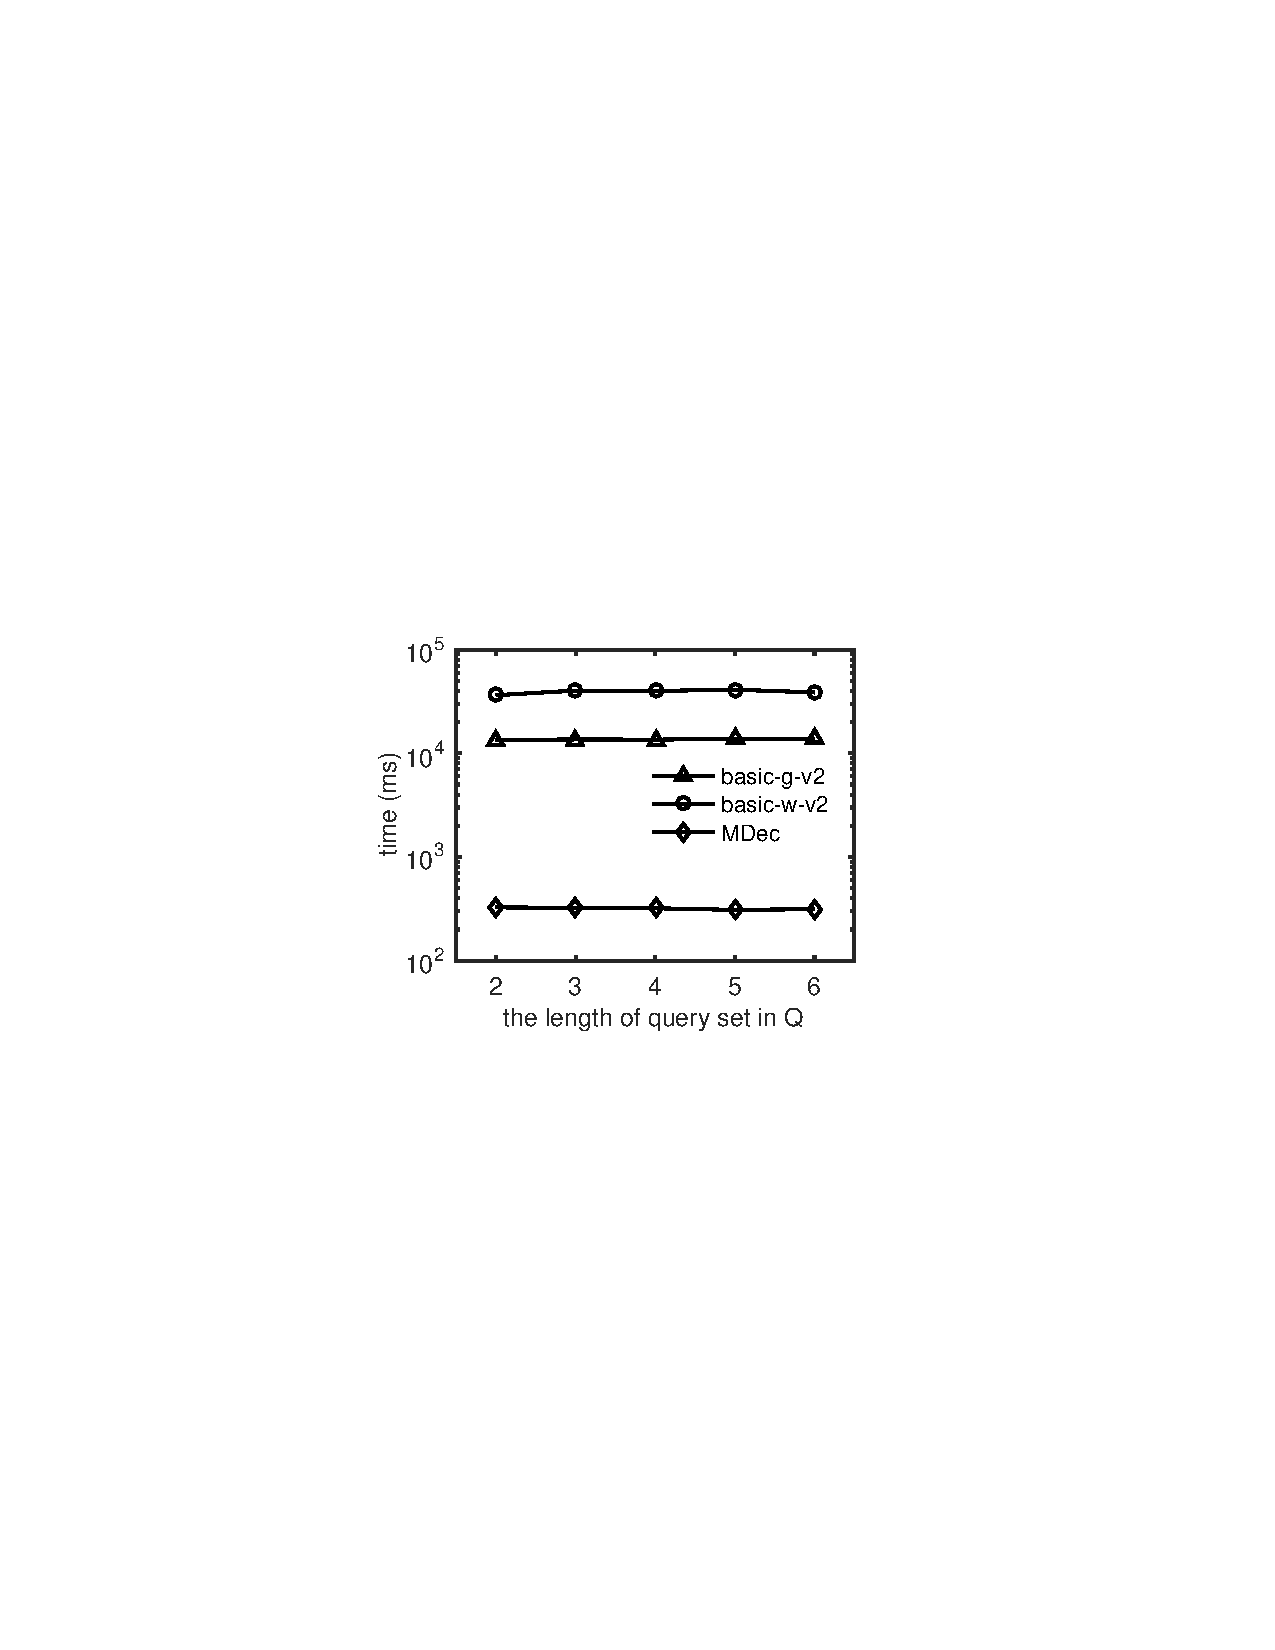
\includegraphics[width=3.725cm]{figures/tencentv2}
  \end{minipage}
  &
  \begin{minipage}{3.325cm}
  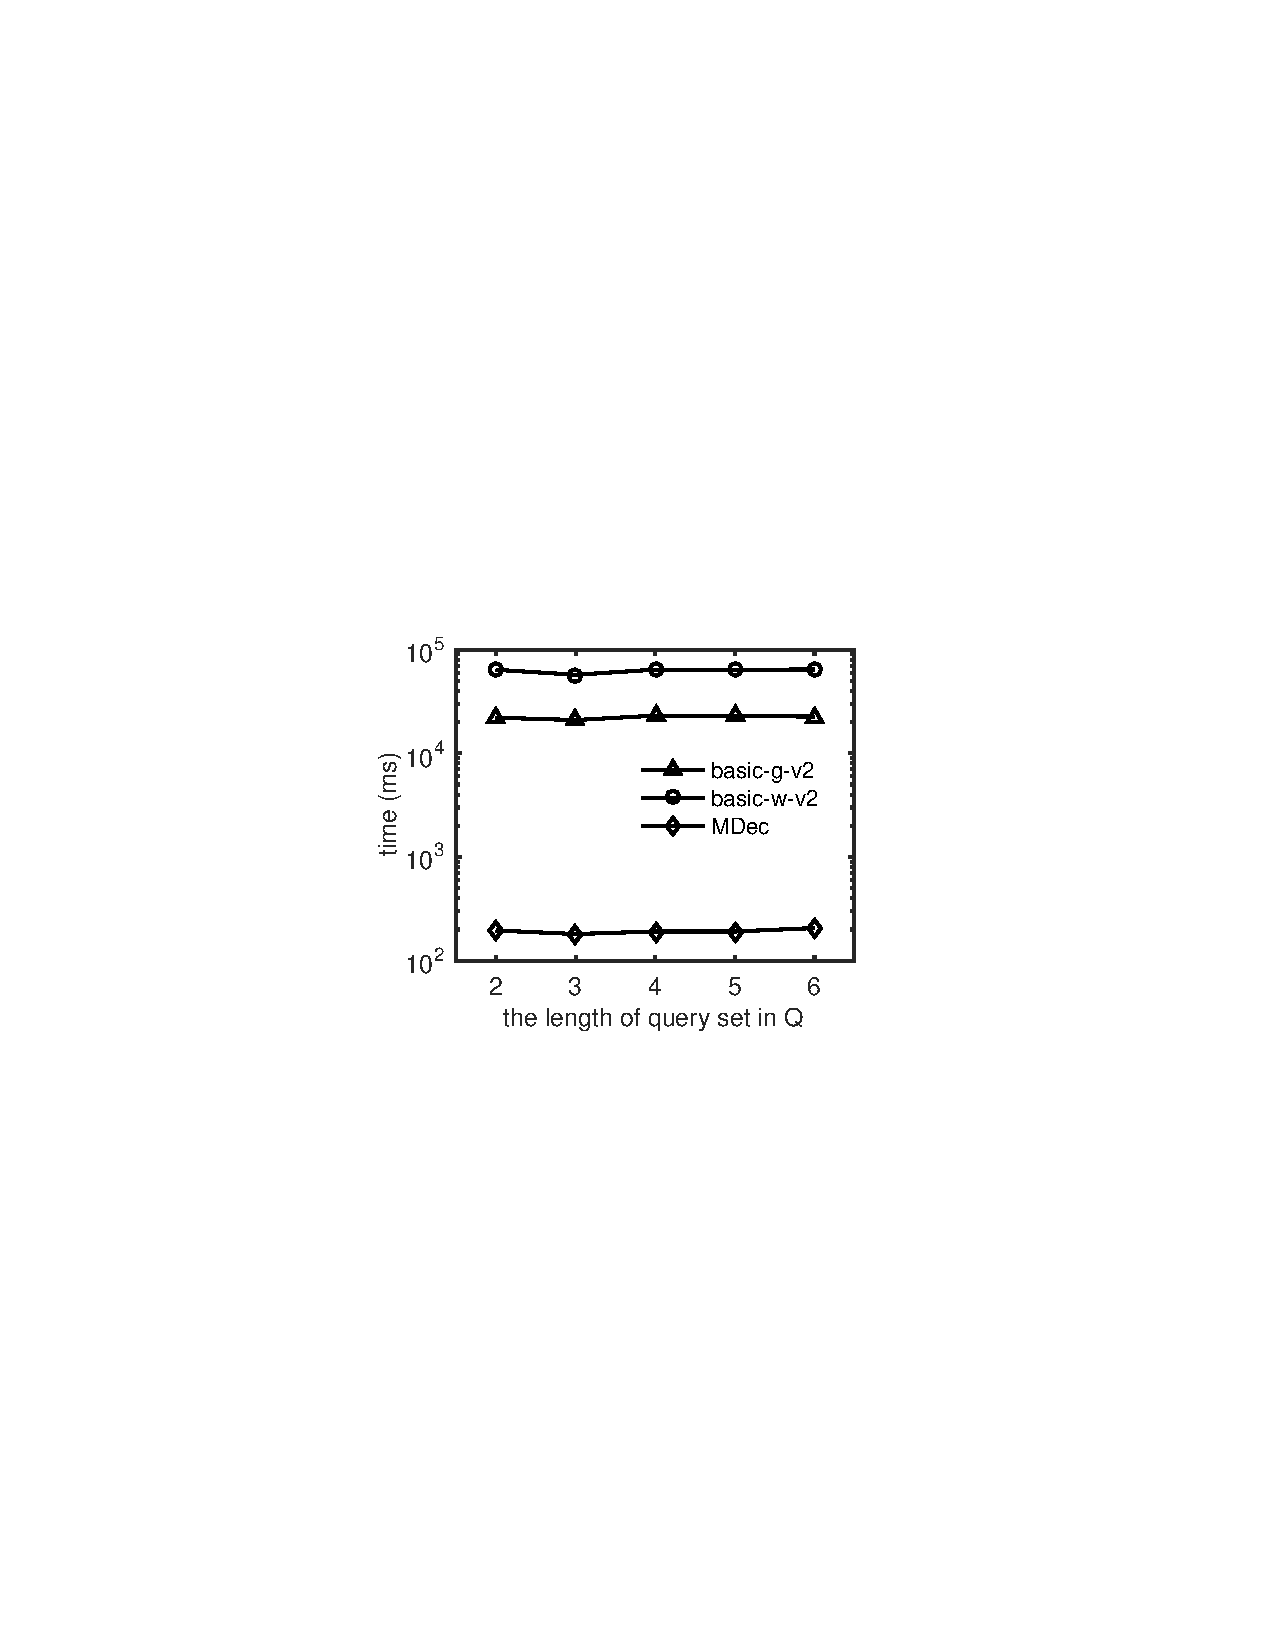
\includegraphics[width=3.725cm]{figures/dbpediav2}
  \end{minipage}
  \\
  \small (e) Flickr (Variant 2)
  &
  \small (f) DBLP (Variant 2)
  &
  \small (g) Tencent (Variant 2)
  &
  \small (h) DBpedia (Variant 2)
\\


\end{tabular}
\caption{Efficiency results of Variants of ACQ problem.}
\label{fig:exp-variant}
\end{figure*}


\textbf{8. Effect of invertedList.}
To test the importance of invertedList, we have implemented {\tt Inc-S*} and {\tt Inc-T*}, which are respective variants of {\tt Inc-S} and {\tt Inc-T}, but without the invertedList structure at each CL-tree node. Figure~\ref{fig:exp-more-inverted} shows the results. We see that {\tt Inc-S} ({\tt Inc-T}) is 1 to 2 order of magnitude faster than {\tt Inc-S*} ({\tt Inc-T*}) on all the four datasets in our experiments.
The reason is that the keyword-checking operation mentioned in the above example is frequently performed in the ACQ search process. Thus, the invertedList, which improves the performance of this operation, allows the ACQ search to be conducted more efficiently.

\textbf{9. Non-attributed graphs.}
We have tested {\tt Dec} and {\tt Local} on non-attributed graphs. This is done by running these algorithms on our datasets, without using any of their associated keyword sets. As shown in Figure~\ref{fig:exp-more-decComp}, for Flickr, Tencent and DBpedia, {\tt Dec} is consistently faster than {\tt Local}. In {\tt Dec}, cores are organized into the CL-tree structure. Because the height of the CL-tree is not very high (lower than 405 for all datasets), the core-locating operation can be done quickly. For DBLP, {\tt Dec} is also  faster than {\tt Local}, except when $k$=4. In this dataset, a paper often has few (around 3 to 5) co-authors. Since an author may be closely related to a few co-authors, finding a 4-$\widehat {core}$ in {\tt Local} can be done efficiently through local expansion.  From these experiments, we conclude that {\tt Dec} can also be efficiently executed on non-attributed graphs.

{\color{blue}
\textbf{10. Effect of $\theta$ in Variant 1.}
For each query vertex, we randomly select 10 keywords to form set $S$, set $\theta$ as 0.2, 0.4 0.6, 0.8 and 1.0,
and answer the query of Variant 1 using {\tt basic-g-v1}, {\tt basic-w-v1} and {\tt SWT}.
Figures~\ref{fig:exp-variant}(a)-\ref{fig:exp-variant}(d) show their efficiency.
We can see that {\tt SWT} outperforms the basic solutions consistently, as it uses the CL-tree index.

\textbf{11. Effect of $|Q|$ in Variant 2.}
We randomly select five groups of query sets by varying the size of $Q$ from 2 to 6.
Each group has 200 query sets.
We run {\tt basic-g-v2}, {\tt basic-w-v2} and {\tt MDec} with these five groups of query sets,
and report efficiency in Figures~\ref{fig:exp-variant}(e)-\ref{fig:exp-variant}(h).
Similar to the results of single query vertices, we can observe that {\tt MDec} is at least two orders of magnitude faster than the baseline solutions which do not use the CL-tree index.
}

%\chen{
%\subsection{Experiments on Variants}
%\label{app:varExp}
%\chen{
%The experimental results of variants are presented here and the basic algorithms for these variants are attached in Appendix~\ref{app:algoOfVariant}.
%}
%
%\textbf{1. Case study of Variants 1 and 2.}
%We search Jiawei Han's communities with explicit AC-label constraints in Variants 1 and 2.
%We consider two keyword sets, \textit{i.e.}, $S_1$=$\{$stream, classification$\}$ and $S_2$=$\{$cube, information, cluster$\}$.
%Note that the captions indicate the shared keywords of the communities.
%While for Variant 1 ($\theta$=0.6), we can obtain two communities (see Figures~\ref{fig:jiawei-v1}(a) and~\ref{fig:jiawei-v1}(b)). This implies that, for Variant 1, although we cannot find a community with AC-label being exactly $S_2$, we still can find a community, in which each member contains at least 60\% percentage of keywords of the input query keyword set. And for Variant 2, if the query set is \{Jiawei Han, Jing gao\}, and the keyword set is $S_1$=$\{$stream, classification$\}$, we will also obtain the community in Figures~\ref{fig:jiawei-v1}(a).
%
%
%\begin{figure}[ht]
%    \centering
%    \mbox{
%        \subfigure[$\{$stream, classification$\}$]{
%            \includegraphics[width=.42\columnwidth]{figures/jiawei-v1-1}
%            \label{fig:jiawei-v1-1}
%        }
%        \hspace{1ex}
%        \subfigure[$\{$cube, information$\}$]{
%            \includegraphics[width=.415\columnwidth]{figures/jiawei-v1-2}
%            \label{fig:jiawei-v1-2}
%        }
%    }
%    \caption{Jiawei Han's communities on Variants 1 and 2.}\label{fig:jiawei-v1}
%\end{figure}
%
%
%
%
%\textbf{2. Effect of $\theta$ in Variant 1.}
%For each query vertex, we randomly select 10 keywords to form set $S$, set $\theta$ as 0.2, 0.4 0.6, 0.8 and 1.0,
%and answer the query of Variant 1 using {\tt basic-g-v1}, {\tt basic-w-v1} and {\tt SWT}.
%Figures~\ref{fig:exp-variant}(a)-\ref{fig:exp-variant}(d) show their efficiency.
%We can see that {\tt SWT} outperforms the basic solutions consistently, as it uses the CL-tree index.
%
%{\color{blue}
%\textbf{3. Effect of $|Q|$ in Variant 2.}
%We limit query vertices with no more than 6 keywords.
%We randomly select 2, 3, 4, 5, 6 vertices to form the query set, and answer the query of Variant 2 using {\tt basic-g-v2}, {\tt basic-w-v2} and {\tt MDec}. Figures~\ref{fig:exp-variant}(e)-\ref{fig:exp-variant}(h) show their efficiency. Similar with Variant 2, we can see that {\tt MDec} performs the best by using the CL-tree index.
%}
%
%} 